% Generated by Sphinx.
\def\sphinxdocclass{report}
\documentclass[letterpaper,10pt,english]{sphinxmanual}
\usepackage[utf8]{inputenc}
\DeclareUnicodeCharacter{00A0}{\nobreakspace}
\usepackage{cmap}
\usepackage[T1]{fontenc}
\usepackage{babel}
\usepackage{times}
\usepackage[Bjarne]{fncychap}
\usepackage{longtable}
\usepackage{sphinx}
\usepackage{multirow}

\usepackage{dsfont}
\usepackage{slashed}
\usepackage{yfonts}
\usepackage{mathrsfs}
\def\degrees{^\circ}
\def\d{{\rm d}}

\usepackage{color}
\setcounter{tocdepth}{2}

\def\sign{\mathop{\mathrm{sign}}}
\def\L{{\mathcal L}}
\def\H{{\mathcal H}}
\def\M{{\mathcal M}}
\def\matrix{}
\def\fslash#1{#1 \!\!\!/}
\def\F{{\bf F}}
\def\R{{\bf R}}
\def\J{{\bf J}}
\def\x{{\bf x}}
\def\y{{\bf y}}
\def\h{{\rm h}}
\def\a{{\rm a}}
\newcommand{\bfx}{\mbox{\boldmath $x$}}
\newcommand{\bfy}{\mbox{\boldmath $y$}}
\newcommand{\bfz}{\mbox{\boldmath $z$}}
\newcommand{\bfv}{\mbox{\boldmath $v$}}
\newcommand{\bfu}{\mbox{\boldmath $u$}}
\newcommand{\bfF}{\mbox{\boldmath $F$}}
\newcommand{\bfJ}{\mbox{\boldmath $J$}}
\newcommand{\bfU}{\mbox{\boldmath $U$}}
\newcommand{\bfY}{\mbox{\boldmath $Y$}}
\newcommand{\bfR}{\mbox{\boldmath $R$}}
\newcommand{\bfg}{\mbox{\boldmath $g$}}
\newcommand{\bfc}{\mbox{\boldmath $c$}}
\newcommand{\bfxi}{\mbox{\boldmath $\xi$}}

\newcommand{\bra}[1]{\left\langle #1\right|}
\newcommand{\ket}[1]{\left| #1\right\rangle}
\newcommand{\braket}[2]{\langle #1 \mid #2 \rangle}
\newcommand{\avg}[1]{\left< #1 \right>}

%\def\back{\!\!\!\!\!\!\!\!\!\!}
\def\back{}
\def\col#1#2{\left(\matrix{#1#2}\right)}
\def\row#1#2{\left(\matrix{#1#2}\right)}
\def\mat#1{\begin{pmatrix}#1\end{pmatrix}}
\def\matd#1#2{\left(\matrix{#1\back0\cr0\back#2}\right)}
\def\p#1#2{{\partial#1\over\partial#2}}
\def\cg#1#2#3#4#5#6{({#1},\,{#2},\,{#3},\,{#4}\,|\,{#5},\,{#6})}
\def\half{{\textstyle{1\over2}}}
\def\jsym#1#2#3#4#5#6{\left\{\matrix{
{#1}{#2}{#3}
{#4}{#5}{#6}
}\right\}}
\def\diag{\hbox{diag}}

\font\dsrom=dsrom10
\def\one{\hbox{\dsrom 1}}

\def\res{\mathop{\mathrm{Res}}}

\def\mathnot#1{\text{"$#1$"}}


%See Character Table for cmmib10:
%http://www.math.union.edu/~dpvc/jsmath/download/extra-fonts/cmmib10/cmmib10.html
\font\mib=cmmib10
\def\balpha{\hbox{\mib\char"0B}}
\def\bbeta{\hbox{\mib\char"0C}}
\def\bgamma{\hbox{\mib\char"0D}}
\def\bdelta{\hbox{\mib\char"0E}}
\def\bepsilon{\hbox{\mib\char"0F}}
\def\bzeta{\hbox{\mib\char"10}}
\def\boldeta{\hbox{\mib\char"11}}
\def\btheta{\hbox{\mib\char"12}}
\def\biota{\hbox{\mib\char"13}}
\def\bkappa{\hbox{\mib\char"14}}
\def\blambda{\hbox{\mib\char"15}}
\def\bmu{\hbox{\mib\char"16}}
\def\bnu{\hbox{\mib\char"17}}
\def\bxi{\hbox{\mib\char"18}}
\def\bpi{\hbox{\mib\char"19}}
\def\brho{\hbox{\mib\char"1A}}
\def\bsigma{\hbox{\mib\char"1B}}
\def\btau{\hbox{\mib\char"1C}}
\def\bupsilon{\hbox{\mib\char"1D}}
\def\bphi{\hbox{\mib\char"1E}}
\def\bchi{\hbox{\mib\char"1F}}
\def\bpsi{\hbox{\mib\char"20}}
\def\bomega{\hbox{\mib\char"21}}

\def\bvarepsilon{\hbox{\mib\char"22}}
\def\bvartheta{\hbox{\mib\char"23}}
\def\bvarpi{\hbox{\mib\char"24}}
\def\bvarrho{\hbox{\mib\char"25}}
\def\bvarphi{\hbox{\mib\char"27}}

%how to use:
%$$\alpha\balpha$$
%$$\beta\bbeta$$
%$$\gamma\bgamma$$
%$$\delta\bdelta$$
%$$\epsilon\bepsilon$$
%$$\zeta\bzeta$$
%$$\eta\boldeta$$
%$$\theta\btheta$$
%$$\iota\biota$$
%$$\kappa\bkappa$$
%$$\lambda\blambda$$
%$$\mu\bmu$$
%$$\nu\bnu$$
%$$\xi\bxi$$
%$$\pi\bpi$$
%$$\rho\brho$$
%$$\sigma\bsigma$$
%$$\tau\btau$$
%$$\upsilon\bupsilon$$
%$$\phi\bphi$$
%$$\chi\bchi$$
%$$\psi\bpsi$$
%$$\omega\bomega$$
%
%$$\varepsilon\bvarepsilon$$
%$$\vartheta\bvartheta$$
%$$\varpi\bvarpi$$
%$$\varrho\bvarrho$$
%$$\varphi\bvarphi$$

%small font
\font\mibsmall=cmmib7
\def\bsigmasmall{\hbox{\mibsmall\char"1B}}

\def\Tr{\hbox{Tr}\,}
\def\Arg{\hbox{Arg}}
\def\atan{\hbox{atan}}


\title{Statistical Physics Notes}
\date{October 04, 2014}
\release{1.38}
\author{Lei Ma}
\newcommand{\sphinxlogo}{}
\renewcommand{\releasename}{Release}
\makeindex

\makeatletter
\def\PYG@reset{\let\PYG@it=\relax \let\PYG@bf=\relax%
    \let\PYG@ul=\relax \let\PYG@tc=\relax%
    \let\PYG@bc=\relax \let\PYG@ff=\relax}
\def\PYG@tok#1{\csname PYG@tok@#1\endcsname}
\def\PYG@toks#1+{\ifx\relax#1\empty\else%
    \PYG@tok{#1}\expandafter\PYG@toks\fi}
\def\PYG@do#1{\PYG@bc{\PYG@tc{\PYG@ul{%
    \PYG@it{\PYG@bf{\PYG@ff{#1}}}}}}}
\def\PYG#1#2{\PYG@reset\PYG@toks#1+\relax+\PYG@do{#2}}

\expandafter\def\csname PYG@tok@gd\endcsname{\def\PYG@tc##1{\textcolor[rgb]{0.63,0.00,0.00}{##1}}}
\expandafter\def\csname PYG@tok@gu\endcsname{\let\PYG@bf=\textbf\def\PYG@tc##1{\textcolor[rgb]{0.50,0.00,0.50}{##1}}}
\expandafter\def\csname PYG@tok@gt\endcsname{\def\PYG@tc##1{\textcolor[rgb]{0.00,0.27,0.87}{##1}}}
\expandafter\def\csname PYG@tok@gs\endcsname{\let\PYG@bf=\textbf}
\expandafter\def\csname PYG@tok@gr\endcsname{\def\PYG@tc##1{\textcolor[rgb]{1.00,0.00,0.00}{##1}}}
\expandafter\def\csname PYG@tok@cm\endcsname{\let\PYG@it=\textit\def\PYG@tc##1{\textcolor[rgb]{0.25,0.50,0.56}{##1}}}
\expandafter\def\csname PYG@tok@vg\endcsname{\def\PYG@tc##1{\textcolor[rgb]{0.73,0.38,0.84}{##1}}}
\expandafter\def\csname PYG@tok@m\endcsname{\def\PYG@tc##1{\textcolor[rgb]{0.13,0.50,0.31}{##1}}}
\expandafter\def\csname PYG@tok@mh\endcsname{\def\PYG@tc##1{\textcolor[rgb]{0.13,0.50,0.31}{##1}}}
\expandafter\def\csname PYG@tok@cs\endcsname{\def\PYG@tc##1{\textcolor[rgb]{0.25,0.50,0.56}{##1}}\def\PYG@bc##1{\setlength{\fboxsep}{0pt}\colorbox[rgb]{1.00,0.94,0.94}{\strut ##1}}}
\expandafter\def\csname PYG@tok@ge\endcsname{\let\PYG@it=\textit}
\expandafter\def\csname PYG@tok@vc\endcsname{\def\PYG@tc##1{\textcolor[rgb]{0.73,0.38,0.84}{##1}}}
\expandafter\def\csname PYG@tok@il\endcsname{\def\PYG@tc##1{\textcolor[rgb]{0.13,0.50,0.31}{##1}}}
\expandafter\def\csname PYG@tok@go\endcsname{\def\PYG@tc##1{\textcolor[rgb]{0.20,0.20,0.20}{##1}}}
\expandafter\def\csname PYG@tok@cp\endcsname{\def\PYG@tc##1{\textcolor[rgb]{0.00,0.44,0.13}{##1}}}
\expandafter\def\csname PYG@tok@gi\endcsname{\def\PYG@tc##1{\textcolor[rgb]{0.00,0.63,0.00}{##1}}}
\expandafter\def\csname PYG@tok@gh\endcsname{\let\PYG@bf=\textbf\def\PYG@tc##1{\textcolor[rgb]{0.00,0.00,0.50}{##1}}}
\expandafter\def\csname PYG@tok@ni\endcsname{\let\PYG@bf=\textbf\def\PYG@tc##1{\textcolor[rgb]{0.84,0.33,0.22}{##1}}}
\expandafter\def\csname PYG@tok@nl\endcsname{\let\PYG@bf=\textbf\def\PYG@tc##1{\textcolor[rgb]{0.00,0.13,0.44}{##1}}}
\expandafter\def\csname PYG@tok@nn\endcsname{\let\PYG@bf=\textbf\def\PYG@tc##1{\textcolor[rgb]{0.05,0.52,0.71}{##1}}}
\expandafter\def\csname PYG@tok@no\endcsname{\def\PYG@tc##1{\textcolor[rgb]{0.38,0.68,0.84}{##1}}}
\expandafter\def\csname PYG@tok@na\endcsname{\def\PYG@tc##1{\textcolor[rgb]{0.25,0.44,0.63}{##1}}}
\expandafter\def\csname PYG@tok@nb\endcsname{\def\PYG@tc##1{\textcolor[rgb]{0.00,0.44,0.13}{##1}}}
\expandafter\def\csname PYG@tok@nc\endcsname{\let\PYG@bf=\textbf\def\PYG@tc##1{\textcolor[rgb]{0.05,0.52,0.71}{##1}}}
\expandafter\def\csname PYG@tok@nd\endcsname{\let\PYG@bf=\textbf\def\PYG@tc##1{\textcolor[rgb]{0.33,0.33,0.33}{##1}}}
\expandafter\def\csname PYG@tok@ne\endcsname{\def\PYG@tc##1{\textcolor[rgb]{0.00,0.44,0.13}{##1}}}
\expandafter\def\csname PYG@tok@nf\endcsname{\def\PYG@tc##1{\textcolor[rgb]{0.02,0.16,0.49}{##1}}}
\expandafter\def\csname PYG@tok@si\endcsname{\let\PYG@it=\textit\def\PYG@tc##1{\textcolor[rgb]{0.44,0.63,0.82}{##1}}}
\expandafter\def\csname PYG@tok@s2\endcsname{\def\PYG@tc##1{\textcolor[rgb]{0.25,0.44,0.63}{##1}}}
\expandafter\def\csname PYG@tok@vi\endcsname{\def\PYG@tc##1{\textcolor[rgb]{0.73,0.38,0.84}{##1}}}
\expandafter\def\csname PYG@tok@nt\endcsname{\let\PYG@bf=\textbf\def\PYG@tc##1{\textcolor[rgb]{0.02,0.16,0.45}{##1}}}
\expandafter\def\csname PYG@tok@nv\endcsname{\def\PYG@tc##1{\textcolor[rgb]{0.73,0.38,0.84}{##1}}}
\expandafter\def\csname PYG@tok@s1\endcsname{\def\PYG@tc##1{\textcolor[rgb]{0.25,0.44,0.63}{##1}}}
\expandafter\def\csname PYG@tok@gp\endcsname{\let\PYG@bf=\textbf\def\PYG@tc##1{\textcolor[rgb]{0.78,0.36,0.04}{##1}}}
\expandafter\def\csname PYG@tok@sh\endcsname{\def\PYG@tc##1{\textcolor[rgb]{0.25,0.44,0.63}{##1}}}
\expandafter\def\csname PYG@tok@ow\endcsname{\let\PYG@bf=\textbf\def\PYG@tc##1{\textcolor[rgb]{0.00,0.44,0.13}{##1}}}
\expandafter\def\csname PYG@tok@sx\endcsname{\def\PYG@tc##1{\textcolor[rgb]{0.78,0.36,0.04}{##1}}}
\expandafter\def\csname PYG@tok@bp\endcsname{\def\PYG@tc##1{\textcolor[rgb]{0.00,0.44,0.13}{##1}}}
\expandafter\def\csname PYG@tok@c1\endcsname{\let\PYG@it=\textit\def\PYG@tc##1{\textcolor[rgb]{0.25,0.50,0.56}{##1}}}
\expandafter\def\csname PYG@tok@kc\endcsname{\let\PYG@bf=\textbf\def\PYG@tc##1{\textcolor[rgb]{0.00,0.44,0.13}{##1}}}
\expandafter\def\csname PYG@tok@c\endcsname{\let\PYG@it=\textit\def\PYG@tc##1{\textcolor[rgb]{0.25,0.50,0.56}{##1}}}
\expandafter\def\csname PYG@tok@mf\endcsname{\def\PYG@tc##1{\textcolor[rgb]{0.13,0.50,0.31}{##1}}}
\expandafter\def\csname PYG@tok@err\endcsname{\def\PYG@bc##1{\setlength{\fboxsep}{0pt}\fcolorbox[rgb]{1.00,0.00,0.00}{1,1,1}{\strut ##1}}}
\expandafter\def\csname PYG@tok@kd\endcsname{\let\PYG@bf=\textbf\def\PYG@tc##1{\textcolor[rgb]{0.00,0.44,0.13}{##1}}}
\expandafter\def\csname PYG@tok@ss\endcsname{\def\PYG@tc##1{\textcolor[rgb]{0.32,0.47,0.09}{##1}}}
\expandafter\def\csname PYG@tok@sr\endcsname{\def\PYG@tc##1{\textcolor[rgb]{0.14,0.33,0.53}{##1}}}
\expandafter\def\csname PYG@tok@mo\endcsname{\def\PYG@tc##1{\textcolor[rgb]{0.13,0.50,0.31}{##1}}}
\expandafter\def\csname PYG@tok@mi\endcsname{\def\PYG@tc##1{\textcolor[rgb]{0.13,0.50,0.31}{##1}}}
\expandafter\def\csname PYG@tok@kn\endcsname{\let\PYG@bf=\textbf\def\PYG@tc##1{\textcolor[rgb]{0.00,0.44,0.13}{##1}}}
\expandafter\def\csname PYG@tok@o\endcsname{\def\PYG@tc##1{\textcolor[rgb]{0.40,0.40,0.40}{##1}}}
\expandafter\def\csname PYG@tok@kr\endcsname{\let\PYG@bf=\textbf\def\PYG@tc##1{\textcolor[rgb]{0.00,0.44,0.13}{##1}}}
\expandafter\def\csname PYG@tok@s\endcsname{\def\PYG@tc##1{\textcolor[rgb]{0.25,0.44,0.63}{##1}}}
\expandafter\def\csname PYG@tok@kp\endcsname{\def\PYG@tc##1{\textcolor[rgb]{0.00,0.44,0.13}{##1}}}
\expandafter\def\csname PYG@tok@w\endcsname{\def\PYG@tc##1{\textcolor[rgb]{0.73,0.73,0.73}{##1}}}
\expandafter\def\csname PYG@tok@kt\endcsname{\def\PYG@tc##1{\textcolor[rgb]{0.56,0.13,0.00}{##1}}}
\expandafter\def\csname PYG@tok@sc\endcsname{\def\PYG@tc##1{\textcolor[rgb]{0.25,0.44,0.63}{##1}}}
\expandafter\def\csname PYG@tok@sb\endcsname{\def\PYG@tc##1{\textcolor[rgb]{0.25,0.44,0.63}{##1}}}
\expandafter\def\csname PYG@tok@k\endcsname{\let\PYG@bf=\textbf\def\PYG@tc##1{\textcolor[rgb]{0.00,0.44,0.13}{##1}}}
\expandafter\def\csname PYG@tok@se\endcsname{\let\PYG@bf=\textbf\def\PYG@tc##1{\textcolor[rgb]{0.25,0.44,0.63}{##1}}}
\expandafter\def\csname PYG@tok@sd\endcsname{\let\PYG@it=\textit\def\PYG@tc##1{\textcolor[rgb]{0.25,0.44,0.63}{##1}}}

\def\PYGZbs{\char`\\}
\def\PYGZus{\char`\_}
\def\PYGZob{\char`\{}
\def\PYGZcb{\char`\}}
\def\PYGZca{\char`\^}
\def\PYGZam{\char`\&}
\def\PYGZlt{\char`\<}
\def\PYGZgt{\char`\>}
\def\PYGZsh{\char`\#}
\def\PYGZpc{\char`\%}
\def\PYGZdl{\char`\$}
\def\PYGZhy{\char`\-}
\def\PYGZsq{\char`\'}
\def\PYGZdq{\char`\"}
\def\PYGZti{\char`\~}
% for compatibility with earlier versions
\def\PYGZat{@}
\def\PYGZlb{[}
\def\PYGZrb{]}
\makeatother

\begin{document}

\maketitle
\tableofcontents
\phantomsection\label{index::doc}


A note recording project for stat mech course.

\textbf{Progress}: 15/15


\chapter{Acknowledgement}
\label{index:statistical-mechanics}\label{index:acknowledgement}
I have finished the whole set of notes for my statistical mechanics class which is taught by V. M. Kenkre 2014 Spring.

Professor Kenkre's lectures are as fantastic as an excellent thrilling movie without which I could never finish notes like this. I am very grateful to him for this adventure to modern statistical mechanics. The words I can think of to describe these lectures are the words used on the best chinese novel, \emph{Dream of the Red Chamber}:

{\hfill
\includegraphics{aComment.png}\hfill}

which is too hard to translate. It basically means that the subplot permeats through thousands of pages before people realize it's importance. Professor's Kenkre's lectures do have such power that a tiny hint could develop to an important idea as the lectures go on.

I am also very grateful to the TA of this course, \href{http://www.unm.edu/~aierides/505/}{Anastasia}, who helped me a lot with my homework and lecture notes.


\chapter{Introduction}
\label{index:introduction}
Statistical Physics is the central topic of physics. It taught us great lessons about nature and it is definitely going to teach us more. Some ideas (Verlinde's scenario) even put thermodynamics and statistical physics as the fundamental of all theories thus the thought that everything is emergent has been announced.

Basically, statistical mechanics is the mechanics of large bodies.
\begin{itemize}
\item {} 
Mechanics is Newton's plan of kinematics.

\item {} 
Large means a lot of DoFs. Usually DoFs add up to $10^{23}$ which is the order of Avogadro's number.

\item {} 
Bodies, of course, is the subject or system we are dealing with.

\end{itemize}

One question worth thinking about is how we end up with probabilities.

We wouldn't need probability theory if we carry out Newton's plan exactly. Note that the first thing we drop to come over the obstacles is to drop initial condition because it's impossible to write down the initial condition of a large system for each particle. The price of that is we have to use probability to describe the system. Later on we find out that some dynamics have to be dropped to make it calculable which then gives us other sources of probability.

\textbf{It's kind of disappointing that stat mech is so vague. I feel unsafe.}


\chapter{Vocabulary}
\label{index:vocabulary}

\section{Vocabulary and Program}
\label{vocabulary/main:vocabulary-and-program}\label{vocabulary/main::doc}
\index{Gaussian Integral}\index{Special Functions}

\subsection{Vocabulary}
\label{vocabulary/vocabulary:index-0}\label{vocabulary/vocabulary::doc}\label{vocabulary/vocabulary:vocabulary}
\index{Gaussian Integral}

\subsubsection{Gaussian Intergral}
\label{vocabulary/vocabulary:index-1}\label{vocabulary/vocabulary:gaussian-intergral}\begin{gather}
\begin{split}\int_{-\infty}^{\infty} e^{-ax^2} \mathrm dx = \sqrt{\frac{\pi}{a}}\end{split}\notag
\end{gather}
A comprehensive description of how this is done is \href{http://mathworld.wolfram.com/GaussianIntegral.html}{here}.

Basicly, we just transform the problem to the $\int e^{-x} \mathrm dx$ problem.


\subsubsection{Behavior of Functions}
\label{vocabulary/vocabulary:behavior-of-functions}\begin{enumerate}
\setcounter{enumi}{-1}
\item {} 
Boltzmann factor

\end{enumerate}

The most important and weirdest function in statmech

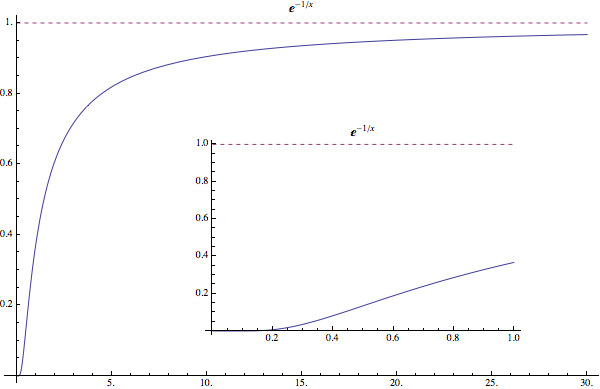
\includegraphics[width=0.800\linewidth]{boltzfactor1.png}
\begin{enumerate}
\item {} 
Tanh(x)

\end{enumerate}

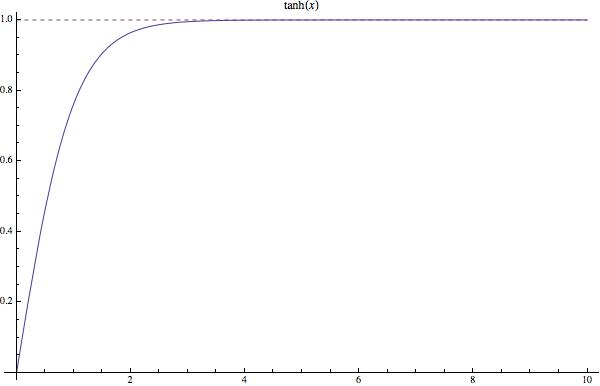
\includegraphics[width=0.800\linewidth]{tanh1.jpg}
\begin{enumerate}
\setcounter{enumi}{1}
\item {} 
$1-exp(-x)$

\end{enumerate}

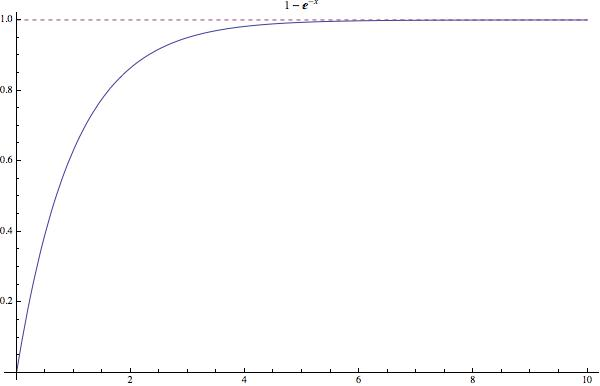
\includegraphics[width=0.800\linewidth]{exp11.jpg}
\begin{enumerate}
\setcounter{enumi}{2}
\item {} 
$cosh(1/x)-1/x$

\end{enumerate}

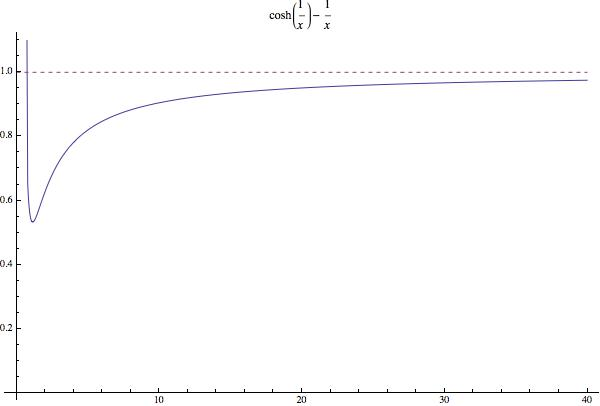
\includegraphics[width=0.800\linewidth]{cosh11.jpg}
\begin{enumerate}
\setcounter{enumi}{3}
\item {} 
$1/(1+1/x)$

\end{enumerate}

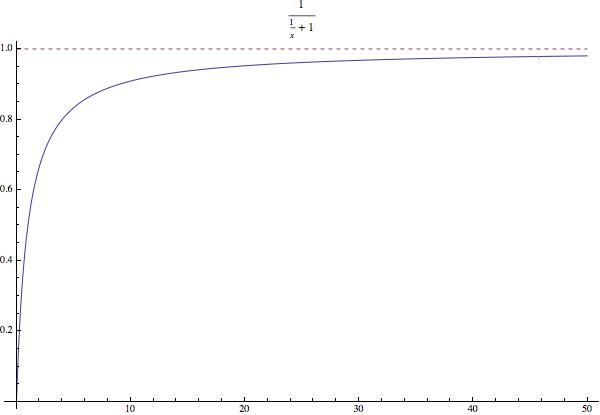
\includegraphics[width=0.800\linewidth]{fraction11.jpg}


\subsubsection{Fourier Transform}
\label{vocabulary/vocabulary:fourier-transform}
Fourier transform for continuous equation is
\begin{gather}
\begin{split}\frac{\partial}{\partial x} e^{ikx}=ike^{ikx} &\implies \frac{\partial}{\partial x} \to ik \\
\frac{\partial^2}{\partial x^2} e^{ikx} = -k^2 e^{ikx} & \implies \frac{\partial^2}{\partial x^2} \to -k^2\end{split}\notag\\\begin{split}\end{split}\notag
\end{gather}

\subsubsection{Laplace Transform}
\label{vocabulary/vocabulary:laplace-transform}
Laplace transform is a transform of a function $f(t)$ to a function of $s$,
\begin{gather}
\begin{split}L[f(t)] = \int_0^\infty f(t) e^{ - s t} dt .\end{split}\notag\\\begin{split}\end{split}\notag
\end{gather}
Some useful properties:
\begin{enumerate}
\item {} 
$L[\frac{d}{dt}f(t)] = s L[f(t)] - f(0)$;

\item {} 
:math:{\color{red}\bfseries{}{}`}L{[}frac\{d\textasciicircum{}2\}\{dt\textasciicircum{}2\}f(t) = s\textasciicircum{}2 L{[}f(t){]} - s f(0) - frac\{d f(0)\}\{dt\} {\color{red}\bfseries{}{}`};

\item {} 
$L[\int_0^t g(\tau) d\tau ] = \frac{L[f(t)]}{s}$;

\item {} 
$L[\alpha t] = \frac{1}{\alpha} L[s/\alpha]$;

\item {} 
$L[e^{at}f(t)] = L[f(s-a)]$;

\item {} 
$L[tf(t)] = - \frac{d}{ds} L[f(t)]$.

\end{enumerate}

Some useful results:
\begin{enumerate}
\item {} 
$L[1] = \frac{1}{s}$;

\item {} 
$L[\delta] = 1$;

\item {} 
$L[\delta^k] = s^k$;

\item {} 
$L[t] = \frac{1}{s^2}$;

\item {} 
$L[e^{at}]= \frac{1}[s-a]$.

\end{enumerate}

A very nice property of Laplace transform is
\begin{gather}
\begin{split}L_s [e^{at}f(t)] &= \int_0^\infty e^{-st} e^{-at} f(t) dt \\
& =  \int_0^\infty e^{-(s+a)t}f(t) dt \\
& = L_{s+a}[f(t)]\end{split}\notag\\\begin{split}\end{split}\notag
\end{gather}
which is very useful when dealing with master equations.

Two useful results are
\begin{gather}
\begin{split}L[I_0(2Ft)] = \frac{1}{\sqrt{ \epsilon^2 - (2F)^2 }}\end{split}\notag\\\begin{split}\end{split}\notag
\end{gather}
and
\begin{gather}
\begin{split}L[J_0[2Ft]]  = \frac{1}{\sqrt{\epsilon^2 + (2F)^2}},\end{split}\notag\\\begin{split}\end{split}\notag
\end{gather}
where $I_0(2Ft)$ is the modified Bessel functions of the first kind. $J_0(2Ft)$ is its companion.

Using the property above, we can find out
\begin{gather}
\begin{split}L[I_0(2Ft)e^{-2Ft}]  = \frac{1}{\sqrt{(\epsilon + 2F)^2 - (2F)^2}} .\end{split}\notag\\\begin{split}\end{split}\notag
\end{gather}

\subsubsection{Functions that will saturate}
\label{vocabulary/vocabulary:functions-that-will-saturate}\begin{gather}
\begin{split}1-e^{-\alpha x}
\tanh(x)
\cosh(\frac{1}{x}) - \frac{1}{x}\end{split}\notag\\\begin{split}\end{split}\notag
\end{gather}

\subsubsection{Legendre Transform}
\label{vocabulary/vocabulary:legendre-transform}
The geometrical of physical meaning of Legendre transformation in thermodynamics can be illustrated by the following graph.

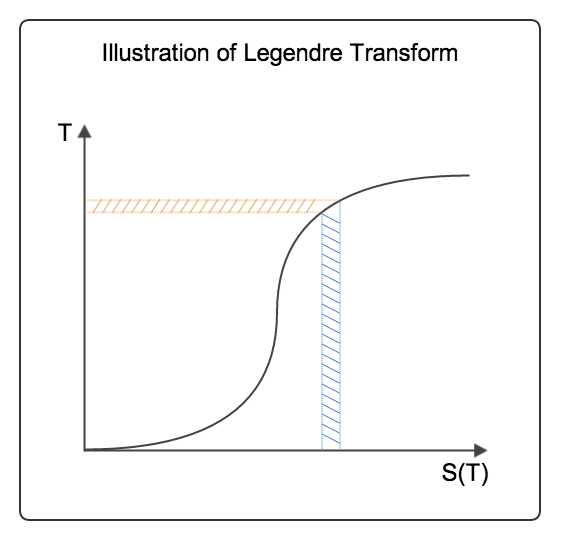
\includegraphics[width=0.800\linewidth]{LegendreTransform.png}

For example, we know that entropy $S$ is actually a function of temperature $T$. For simplicity, we assume that they are monotonically related like in the graph above. When we are talking about the quantity $T \mathrm d S$ we actually mean the area shaded with blue grid lines. Meanwhile the area shaded with orange line means $S \mathrm d T$.

Let's think about the change in internal energy which only the thermal part are considered here, that is,
\begin{gather}
\begin{split}\mathrm d U = T \mathrm d S  .\end{split}\notag\\\begin{split}\end{split}\notag
\end{gather}
So internal energy change is equal to the the area shaded with blue lines. Now think about a three dimensional graph with a third axis of internal energy which I can't show here. Notice that the line of internal energy is on the plane which is vertical to ${T, S}$ plane and contains the line black line in the graph above. The change of internal energy with an increase of $\mathrm dS$ is the value that the line of internal energy goes up.

Now we do such a transform that we actually remove the internal energy from $\mathrm d ( T S )$, which finally gives us Helmholtz free energy,
\begin{gather}
\begin{split}\mathrm d A = S \mathrm d T .\end{split}\notag\\\begin{split}\end{split}\notag
\end{gather}
It's obvious that after this Legendre transform, the new area is the part shaded with orange lines.

Now the key point is that $S(T)$ is a function of $T$. So if we know the blue area then we can find out the orange area, which means that the two function $A(T)$ and $U(S)$ are identical. Choosing one of them for a specific calculation is a kind of freedom and won't change the final results.


\bigskip\hrule{}\bigskip



\bigskip\hrule{}\bigskip



\subsubsection{Thermodynamics}
\label{vocabulary/vocabulary:thermodynamics}
Thermodynamics is about the desciption of large systems which is mostly about the following keypoints. (\emph{A Modern Course in Statistical Physics} by L. E. Reichl)
\begin{enumerate}
\item {} 
Thermodynamic variables; extensive, intensive, neither;

\item {} 
Equations of state;

\item {} 
Four fundamental laws of thermodynamics;

\item {} 
Thermodynamics potentials

\item {} 
Phase transitions

\item {} 
Response

\item {} 
Stability

\end{enumerate}

Anyway, thermodynamics is a kind of theory that deals with black boxes. We manipulate any variables we like and look at the changes. Then we summarize and get a set of laws.

\index{Laws of Thermodynamics}

\paragraph{The Laws of Four}
\label{vocabulary/vocabulary:the-laws-of-four}\label{vocabulary/vocabulary:index-2}
\begin{notice}{note}{Laws}

\textbf{Zeroth} Law: A first feeling about temperature

Two bodies, each in thermodynamic equilibrium with a third system, are in thermodynamic equilibirum with each other.

This gives us the idea that there is a universal quantity which depends only on the state of the system no matter what they are made of.
\end{notice}

\begin{notice}{note}{Laws}

\textbf{First} Law: Conservation of energy

Energy can be transfered or transformed, but can not be destroyed.

In math,
\begin{gather}
\begin{split}\mathrm d U  = W + Q\end{split}\notag\\\begin{split}\end{split}\notag
\end{gather}
where $W$ is the energy done to the system, $Q$ is the heat given to the system. A better way to write this is to make up a one-form $\Omega$,
\begin{gather}
\begin{split}\mathbf\Omega \equiv \mathbf d U  - W - Q =0\end{split}\notag\\\begin{split}\end{split}\notag
\end{gather}
Using Legendre transformation, we know that this one form have many different formalism
\end{notice}

\begin{notice}{note}{Laws}

\textbf{Second} Law: Entropy change; Heat flow direction; Efficieny of heat engine

There are three different versions of this second law. Instead of statements, I would like to use two inequalities to demonstrate this law.
\begin{gather}
\begin{split}\eta = \frac{\Delta W}{\Delta Q} \le 1\end{split}\notag\\\begin{split}\end{split}\notag
\end{gather}
For isolated systems,
\begin{gather}
\begin{split}\mathrm d S \ge 0\end{split}\notag\\\begin{split}\end{split}\notag
\end{gather}
Combine second law with first law, for reversible systems, $W = T\mathbf {\mathrm d} S$, then for ideal gas
\begin{gather}
\begin{split}\mathbf\Omega \equiv \mathbf d U  - T \mathbf  d S + p \mathbf d V =0\end{split}\notag\\\begin{split}\end{split}\notag
\end{gather}
Take the exterior derivative of the whole one-form, and notice that $U$ is exact,
\begin{gather}
\begin{split}-\frac{\partial T}{\partial V}\vert_S \mathbf d V \wedge \mathbf d S + \frac{\partial p}{\partial S}\vert_S \mathbf d S \wedge \mathbf d V = 0\end{split}\notag\\\begin{split}\end{split}\notag
\end{gather}
Clean up this equation we will get one of the Maxwell relations. Use Legendre transformation we can find out all the Maxwell relations.
\end{notice}

\begin{notice}{note}{Laws}

\textbf{Third} Law: Abosoulte zero; Not an extrapolation; Quantum view

The difference in entropy between states connected by a reserible process goes to zero in the limit $T\rightarrow 0 K$.

Due to the asymptotic behavior, one can not get to absolute zero in a finite process.
\end{notice}

\index{Thermodynamics Potentials}

\paragraph{Thermodynamic Potentials}
\label{vocabulary/vocabulary:thermodynamic-potentials}\label{vocabulary/vocabulary:index-3}\begin{enumerate}
\item {} 
Internal Energy

\item {} 
Enthalpy

\item {} 
Helmholtz Free Energy

\item {} 
Gibbs Free Energy

\item {} 
Grand Potential

\end{enumerate}

The relations between them? All potentials are Legendre transformation of each other. To sum up, let's gliffy.

\scalebox{0.800000}{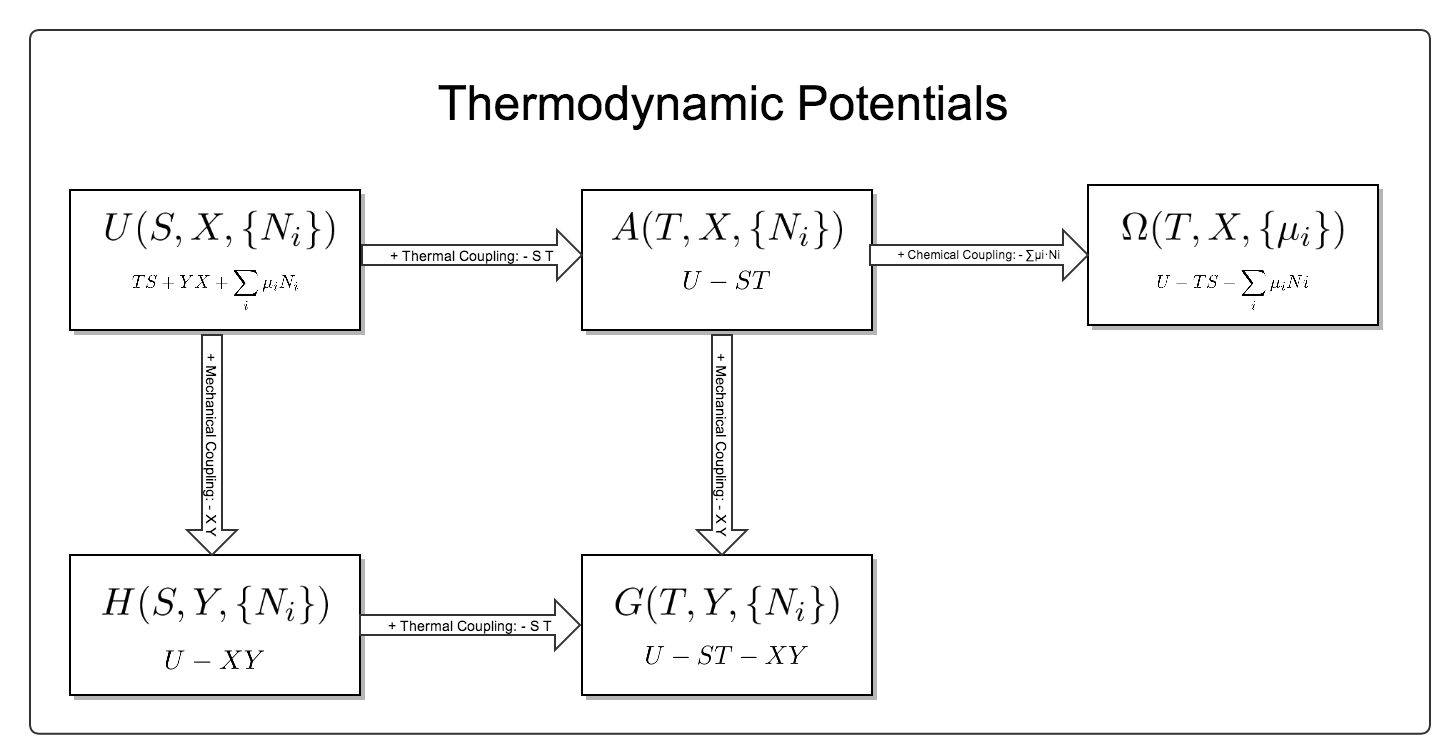
\includegraphics{thermodynamicPotentials1.png}}

(The gliffy source file is here . Feel free to download and create your own version.)

This graph needs some illustration.
\begin{enumerate}
\item {} 
Legendre transformation: $ST-U(S)$ transform a funcion $U(S)$ with variable $S$ to another function $H(T)$. However, in thermodynamics use the different sign can be more convinient. In other words, $U(S)$ and $-H(T)$ are dual to each other.

\item {} 
Starting from this graph, we can find out the differentials of thermodynamic potentials. Next take the partial derivatives of thermodynamic potential with respect to their own variables. By comparing the partial derivatives and the definitions of them, we find out expressions of their vairables. Finally different expressions for the same variable are equal, which are the Maxwell relations.

\item {} 
As we have seen in 2, all the thermodynamic quantities can be obstained by taking the derivatives of thermodynamic potentials.

\end{enumerate}

\begin{notice}{hint}{Hint:}
\textbf{Question:} Mathematically we can construct the sexth potential namely the one that should appear at the right bottom of the graph. Why don't people talk about it?

We can surely define a new potential called $Null(T,X,\{\mu_i\})$. However, the value of this function is zero. So we can have the derivitive of this potential is also zero. This is the Gibbs Duhem equation.

The answer I want to hear is that this is something $\mathrm d\mathrm d f = 0$ where f is exact.
\end{notice}

\index{Entropy}

\paragraph{The Entropy}
\label{vocabulary/vocabulary:index-4}\label{vocabulary/vocabulary:the-entropy}
When talking about entropy, we need to understand the properties of cycles. The most important one is that
\begin{gather}
\begin{split}\sum_{i=1}^n \frac{Q_i}{T_i} \leq 0\end{split}\notag\\\begin{split}\end{split}\notag
\end{gather}
where the equality holds only if the cycle is reversible for the set of processes. In another sense, if we have infinitesimal processes, the equation would have become
\begin{gather}
\begin{split}\oint \frac{\mathrm d Q}{T} = 0 .\end{split}\notag\\\begin{split}\end{split}\notag
\end{gather}
The is an elegent result. It is intuitive that we can build correspondence between one path between two state to any other paths since this is a circle. That being said, the following integral
\begin{gather}
\begin{split}\int_A^B \frac{\mathrm d Q}{T},\end{split}\notag\\\begin{split}\end{split}\notag
\end{gather}
is independent of path on state plane. We imediately define $\int_A^B \frac{\mathrm d Q}{T}$ as a new quantity because we really like invariant quantities in physics, i.e.,
\begin{gather}
\begin{split}S(B) - S(A) = \int_A^B \frac{\mathrm d Q}{T},\end{split}\notag\\\begin{split}\end{split}\notag
\end{gather}
which we call entropy (difference). It is very important to realize that entropy is such a quantity that only dependents on the initial and final state and is independent of path. Many significant results can be derived using only the fact that entropy is a function of state.
\begin{enumerate}
\item {} 
Adiabatic processes on the plane of state never go across each other. Adiabatic lines are isoentropic lines since $\mathrm dS = \frac{\mathrm dQ}{T}$ as $\mathrm dQ = 0$ gives us $\mathrm dS = 0$. The idea is that at the crossing points of adiabatic lines we would get a branch for entropy which means two entropy for one state.

\item {} 
No more than one crossing point of two isothermal lines is possible. To prove it we need to show that entropy is a monotomic equation of $V$.

\item {} 
We can extract heat from one source that has the same temperature and transform into work if the isoentropic lines can cross each other which is not true as entropy is quantity of state. Construct a system with a isothermal line intersects two crossing isoentropic lines.

\item {} 
We can extract heat from low temperature source to high temperature source without causing any other results if we don't have entropy as a quantity of state.

\end{enumerate}


\subsubsection{Refs \& Note}
\label{vocabulary/vocabulary:refs-note}

\subsection{Green Function}
\label{vocabulary/green:green-function}\label{vocabulary/green::doc}
\index{Green Function}

\subsubsection{Green Functions for Second Order Equations}
\label{vocabulary/green:index-0}\label{vocabulary/green:green-functions-for-second-order-equations}
Second order differential equations can be written as
\begin{gather}
\begin{split}L[y] \equiv y'' + p(x) y' + q(x) y = f(x),\end{split}\notag\\\begin{split}\end{split}\notag
\end{gather}
for $a<x<b$ with boundary conditions
\begin{gather}
\begin{split}B_1[y] = B_2[y] = 0.\end{split}\notag\\\begin{split}\end{split}\notag
\end{gather}
The solution is
\begin{gather}
\begin{split}y(x) = \int _a ^b G(x\vert \xi) f(\xi) d\xi\end{split}\notag\\\begin{split}\end{split}\notag
\end{gather}
where Green function is defined as
\begin{gather}
\begin{split}L[G(x\vert \xi)] = \delta(x-\xi)\end{split}\notag\\\begin{split}\end{split}\notag
\end{gather}
with the two boundary conditions,
\begin{gather}
\begin{split}B_1[G] = B_2[G] = 0.\end{split}\notag\\\begin{split}\end{split}\notag
\end{gather}
First order differential of Green function $G'(x\vert \xi)$ has a jump condition at $x=\xi$ that the jump discontinuity of height is 1.


\paragraph{Examples}
\label{vocabulary/green:examples}
2nd DE,
\begin{gather}
\begin{split}y''(x) = f(x), \qquad y(0)= y(1)=0.\end{split}\notag\\\begin{split}\end{split}\notag
\end{gather}
Then Green function for this problem is
\begin{gather}
\begin{split}G''(x\vert \xi) = \delta(x-\xi), \qquad G(0\vert \xi) = G(1\vert \xi) = 0.\end{split}\notag\\\begin{split}\end{split}\notag
\end{gather}
We know the two solutions to the homogeneous equation, $y=1$ or $y=x$. However, only the second solution can satisfy the BC. So Green function should have these properties,
\begin{gather}
\begin{split}G(x\vert \xi) = \begin{cases} c_1+c_2 x &\quad  x<\xi \\ d_1+d_2 x & \quad x>\xi .  \end{cases}\end{split}\notag\\\begin{split}\end{split}\notag
\end{gather}
The BCs give us
\begin{gather}
\begin{split}G(x\vert \xi) = \begin{cases} c x &\quad  x<\xi \\ d(x-1) \quad x>\xi . \end{cases}\end{split}\notag\\\begin{split}\end{split}\notag
\end{gather}
Green functon must be continuous, we have
\begin{gather}
\begin{split}c\xi = d (\xi -1).\end{split}\notag\\\begin{split}\end{split}\notag
\end{gather}
Apply the discontinuity of the first order derivative of Green function,
\begin{gather}
\begin{split}d_x d (x-1)- d_x cx = 1.\end{split}\notag\\\begin{split}\end{split}\notag
\end{gather}
With all these equation, we can determine the Green function,
\begin{gather}
\begin{split}G(x\vert\xi) = \begin{cases}  (\xi -1 ) x , & \qquad x<\xi  \\ \xi(x-1), & \qquad x>\xi  \end{cases}\end{split}\notag\\\begin{split}\end{split}\notag
\end{gather}
Finally we integrate over $\xi$ to get the solution,
\begin{gather}
\begin{split}y(x) &= \int_0^1  G(x\vert \xi) f(\xi) d\xi  \\
& = (x-1)\int_0^x \xi f(\xi) d\xi + x \int_x^1 (\xi -1) f(\xi) d\xi .\end{split}\notag\\\begin{split}\end{split}\notag
\end{gather}
This is the power of Green function.

.


\subsection{Program}
\label{vocabulary/program:program}\label{vocabulary/program::doc}
Most problems in stat mech have similiar procedures. This page is for the programs of solving problems.


\chapter{Equilibrium System}
\label{index:equilibrium-system}

\section{Equilibrium Statistical Mechanics}
\label{equilibrium/main:equilibrium-statistical-mechanics}\label{equilibrium/main::doc}

\subsection{Summary 1}
\label{equilibrium/summary1::doc}\label{equilibrium/summary1:summary-1}
Here is the framework of lectures for the first six weeks. This part is a review of equilibrium statistical mechanics.


\subsubsection{Review of Thermodynamics}
\label{equilibrium/summary1:review-of-thermodynamics}\begin{enumerate}
\item {} 
Description of States: thermodynamics quantities;

\item {} 
Kinematics: Equation of state; Thermodynamics potential
\begin{figure}[htbp]
\centering
\capstart

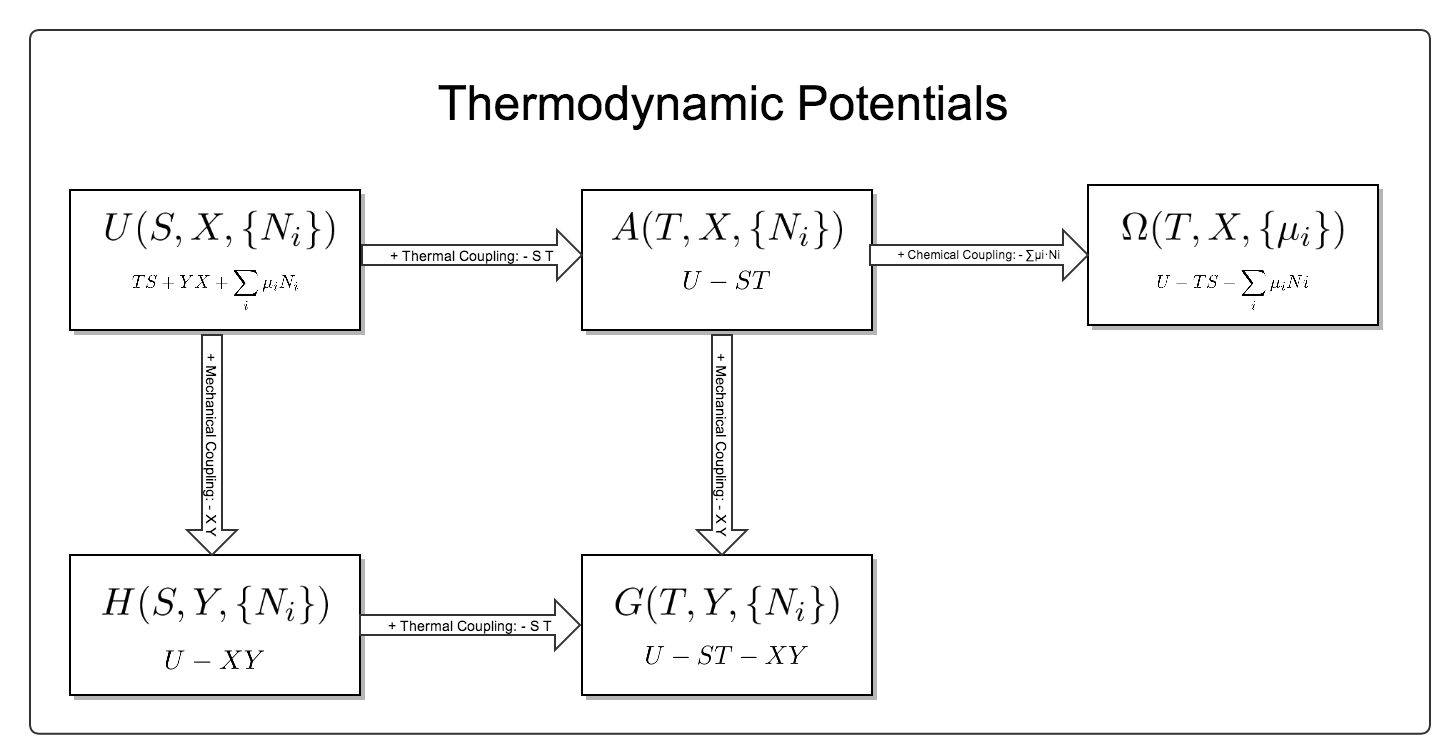
\includegraphics[width=1.000\linewidth]{thermodynamicPotentials.png}
\caption{The relationship between different thermodynamics potential. There are three different couplings and five different potentials. For more details read vocabulary.}\end{figure}

\item {} 
First principles: The laws of four

\item {} 
Dynamics: Phase transition; Stability; Response

\end{enumerate}


\subsubsection{The Two Approaches of Statistical Mechanics}
\label{equilibrium/summary1:the-two-approaches-of-statistical-mechanics}
Two approaches utilize most probable distribution and ensemble respectively. However they have something in common.
\begin{enumerate}
\item {} 
Phase space

\item {} 
Liouville equation

\end{enumerate}
\begin{figure}[htbp]
\centering
\capstart

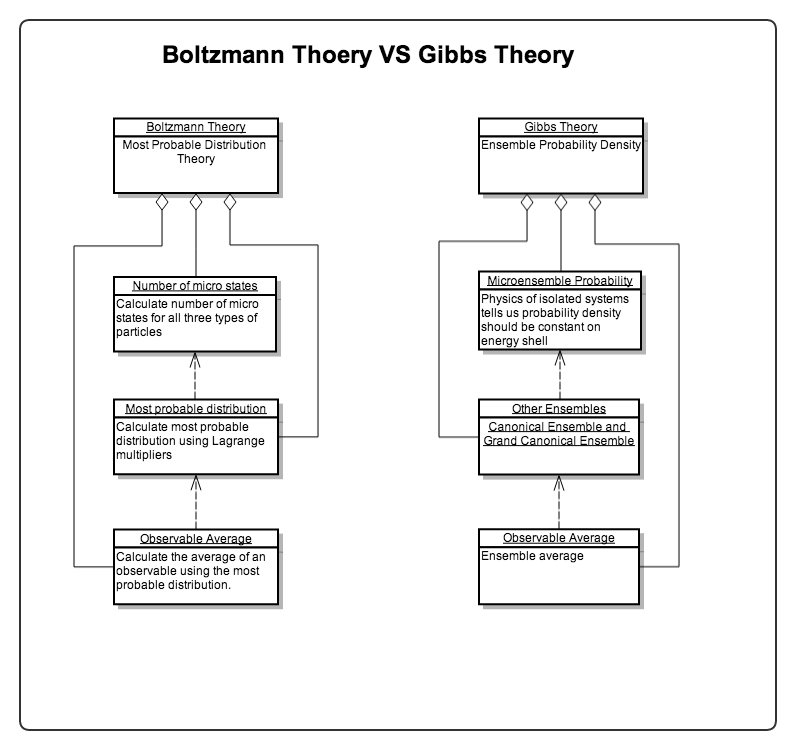
\includegraphics[width=1.000\linewidth]{BoltzmannVSGibbs.png}
\caption{A UML modeling of the two theories. Refer to Important box in week 6}\end{figure}


\paragraph{Boltzmann Statistics}
\label{equilibrium/summary1:boltzmann-statistics}\begin{enumerate}
\item {} 
Two postulates: One is about state occurrence in phase space; The other is about which state will equilibrium system in.

\item {} 
Boltzmann factor (which is kind of derived from Gibbs micro-ensemble theory)

\item {} 
Partition function
\begin{enumerate}
\item {} 
Density of state

\item {} 
Partition function $Z = \int g(E) \exp(-\beta E) \mathrm dE$; Variable of integration can be changed

\item {} 
Systems of 3N DoFs $Z = Z_1^{3N}$

\end{enumerate}

\item {} 
Observable
\begin{enumerate}
\setcounter{enumi}{-1}
\item {} 
Assumptions about free energy $A = - k_B T\ln Z$; Combine this with thermodynamics potential relations we can calculate entropy then everything.

\item {} 
Internal energy $U = \avg{E} = - \partial_\beta \ln Z$; All quantities can be extracted from partition function except those serve as variables of internal energy.

\item {} 
Heat capacity $C = \partial_T U$

\end{enumerate}

\end{enumerate}


\paragraph{Gibbs Ensemble Theory}
\label{equilibrium/summary1:gibbs-ensemble-theory}\begin{enumerate}
\item {} 
Ensembles

\item {} 
Density of states; Liouville equation; Von Neumann equation

\item {} 
Equilibrium

\item {} 
Three ensembles

\item {} 
Observables

\end{enumerate}


\subsubsection{Applications of These Theories}
\label{equilibrium/summary1:applications-of-these-theories}

\paragraph{Oscillators}
\label{equilibrium/summary1:oscillators}
Theories of chains of oscillators in different dimensions are very useful.

A nice practice for this kind of problem is to calculate the heat capacity of diatom chain. A chain of N atom with alternating mass M and m interacting only through nearest neighbors.

The plan for this problem is
\begin{enumerate}
\item {} 
Write down the equation of motion for the whole system;

\item {} 
Fourier transform the system to decouple the modes (find the eigen modes);

\item {} 
Solve the eigen modes;

\item {} 
Calculate the partition function of each mode;

\item {} 
Summation over each mode;

\end{enumerate}

Problem is, we usually can not solve the problem exactly. So we turn to Debye theory. Debye theory assumes continuous spectrum even though our boundary condition quantizes the spectrum. So we need to turn the summation to integration using DoS. There are several ways to obtain DoS. Finally we analyze the different limits to get the low temperature or high temperature behavior.

\begin{notice}{hint}{Hint:}
Here are several methods to obtain DoS.
\end{notice}

\textbf{To do!}


\paragraph{Heat Capacity}
\label{equilibrium/summary1:heat-capacity}\begin{enumerate}
\item {} 
Classical theory: equipartition theorem;

\item {} 
Einstein theory: all modes of oscillations are the same;

\item {} 
Debye theory: different modes of oscillations are considered.

\end{enumerate}


\paragraph{Gibbs Mixing Paradox}
\label{equilibrium/summary1:gibbs-mixing-paradox}
Gibbs mixing paradox is important for the coming in of quantum statistical mechanics.


\paragraph{Mean Field Theory}
\label{equilibrium/summary1:mean-field-theory}
Mean field theory is the idea of treating interaction between particles as interactions between particles and a mean field.


\paragraph{Van der Waals Gas}
\label{equilibrium/summary1:van-der-waals-gas}
Van der Waals gas model can be derived using Mayer expansion and Leonard-Jones potential.

\index{Statistical Mechanics}

\subsection{Week 1}
\label{equilibrium/week1:week-1}\label{equilibrium/week1:index-0}\label{equilibrium/week1::doc}
\index{Statistical Mechanics}\index{Mechanics}\index{Phase Space}\index{Probability}\index{Boltzmann Factor}

\subsubsection{Phase Space}
\label{equilibrium/week1:phase-space}\label{equilibrium/week1:index-1}
Why is statistics important? Remember we are dealing with Avogadro's number of DoFs. If we are going to calculate the dynamics of this system by calculating the dynamics of each particles. To store one screen shot of the system with each DoF take only 8 bits, we need $10^23$ bytes that is $10^17$ GB. It is not even possible to store only one screen shot of the system. So time to change our view of these kind of systems.
\begin{figure}[htbp]
\centering
\capstart

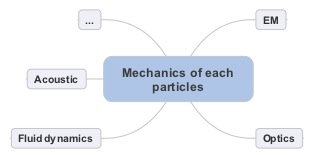
\includegraphics[width=0.600\linewidth]{newtonsDream.jpg}
\caption{Newton's plan of mechanics. Mechanics was in the center of all physics.}\end{figure}

What is mechanics? It deals with dynamics in the following way:
\begin{itemize}
\item {} 
Description of initial state

\item {} 
Time evolution of the system

\item {} 
Extraction of observables

\end{itemize}

As we already mentioned initial state, we need to explain how to describe a state. A vector in phase space gives us a state. Time evolution is motion of points in phase space. Finally, we can do whatever is needed to extract observables, for example just use projection of points in phase space.

Problem is, when it comes to stat mech, it's not possible to do all these DoFs one by one. We need a new concept.


\subsubsection{Boltzmann Factor}
\label{equilibrium/week1:boltzmann-factor}\begin{gather}
\begin{split}\text{probability of a point in phase space} = \exp(-\frac{E}{k_B T})\end{split}\notag
\end{gather}
Boltzmann factor gives us the (not normalized) probability of the system staying on a phase space state with energy $E$.

\begin{notice}{note}{Note:}
Why do Boltzmann factor appear a lot in equilibrium statistical mechanics? Equilibrium of the system means when we add infinitesimal amount of energy to the whole thing including system and reservoir, a characteristic quantity $C(E) = C_S C_R$ won't change. That is the system and the reservoir will have the same changing rate of the characteristic quantity when energy is changed, i.e.,
\begin{gather}
\begin{split}\frac{\partial \ln C_S}{\partial E_S} = - \frac{\partial \ln C_R}{\partial E_R} .\end{split}\notag\\\begin{split}\end{split}\notag
\end{gather}
We have $\mathrm dE_1 = -\mathrm dE_2$ in a equilibrium state. They should both be a constant, which we set to $\beta$. Finally we have something like
\begin{gather}
\begin{split}\frac{\partial \ln C_S}{\partial E_S} = \beta\end{split}\notag\\\begin{split}\end{split}\notag
\end{gather}
which will give us a Boltzmann factor there.

This is just a very simple procedure to show that Boltzmann factor is kind of a natural factor in equilibrium system.
\end{notice}


\subsubsection{Magnetization}
\label{equilibrium/week1:magnetization}
We have such a result in an experiment of magnetization with N magnetic dipoles in 1D.

How can we describe this with a theory?

It's not possible to describe the system by writing down the dynamics of each magnetic dipole. So we have to try some macroscpic view of the system. Probability theory is a great tool for this. The probability of a dipole on a energy state $E_i$ is
\begin{gather}
\begin{split}P(E_i) = \frac{\exp(-\beta E_i)}{\sum_{i=1}^{n} \exp(-\beta E_i)}  .\end{split}\notag\\\begin{split}\end{split}\notag
\end{gather}
So the megnetization in this simple case is
\begin{gather}
\begin{split}M = (\mu N e^{\beta \mu B} - \mu N e^{-\beta \mu B})/(\exp(\beta \mu B) + \exp(-\beta \mu B)) = \mu N \tanh (\beta \mu B)\end{split}\notag\\\begin{split}\end{split}\notag
\end{gather}
Use ipython notebook to display this result. The original notebook can be downloaded from \href{http://emptymalei.github.io/StatisticalPhysics/equilibrium/display.ipynb}{here}. (Just put the link to \href{http://nbviewer.ipython.org}{nbviewer} and everyone can view online.)
\DUspan{operator}{}\DUspan{name}{}\DUspan{name}{}\DUspan{keyword,namespace}{}\DUspan{name,namespace}{}\DUspan{keyword,namespace}{}\DUspan{operator}{}
\begin{Verbatim}[commandchars=\\\{\}]
\%pylab inline
from pylab import *
\end{Verbatim}

\begin{Verbatim}[commandchars=\\\{\}]
Populating the interactive namespace from numpy and matplotlib
\end{Verbatim}
\DUspan{name}{}\DUspan{operator}{}\DUspan{name}{}\DUspan{punctuation}{}\DUspan{literal,number,integer}{}\DUspan{punctuation}{}\DUspan{literal,number,integer}{}\DUspan{punctuation}{}\DUspan{literal,number,integer}{}\DUspan{punctuation}{}\DUspan{name}{}\DUspan{operator}{}\DUspan{name}{}\DUspan{punctuation}{}\DUspan{name}{}\DUspan{punctuation}{}
\begin{Verbatim}[commandchars=\\\{\}]
\PYG{n}{x}\PYG{o}{=}\PYG{n}{linspace}\PYG{p}{(}\PYG{l+m+mi}{0}\PYG{p}{,}\PYG{l+m+mi}{10}\PYG{p}{,}\PYG{l+m+mi}{100}\PYG{p}{)}
\PYG{n}{y}\PYG{o}{=}\PYG{n}{tanh}\PYG{p}{(}\PYG{n}{x}\PYG{p}{)}
\end{Verbatim}
\DUspan{name}{}\DUspan{punctuation}{}\DUspan{name}{}\DUspan{punctuation}{}\DUspan{name}{}\DUspan{punctuation}{}\DUspan{name}{}\DUspan{punctuation}{}\DUspan{literal,string}{}\DUspan{punctuation}{}\DUspan{name}{}\DUspan{punctuation}{}\DUspan{literal,string}{}\DUspan{punctuation}{}\DUspan{name}{}\DUspan{punctuation}{}\DUspan{literal,string}{}\DUspan{punctuation}{}\DUspan{name}{}\DUspan{punctuation}{}\DUspan{literal,string}{}\DUspan{punctuation}{}\DUspan{name}{}\DUspan{punctuation}{}
\begin{Verbatim}[commandchars=\\\{\}]
\PYG{n}{figure}\PYG{p}{(}\PYG{p}{)}
\PYG{n}{plot}\PYG{p}{(}\PYG{n}{x}\PYG{p}{,} \PYG{n}{y}\PYG{p}{,} \PYG{l+s}{\PYGZsq{}}\PYG{l+s}{r}\PYG{l+s}{\PYGZsq{}}\PYG{p}{)}
\PYG{n}{xlabel}\PYG{p}{(}\PYG{l+s}{\PYGZsq{}}\PYG{l+s}{External Magnetic Field}\PYG{l+s}{\PYGZsq{}}\PYG{p}{)}
\PYG{n}{ylabel}\PYG{p}{(}\PYG{l+s}{\PYGZsq{}}\PYG{l+s}{M}\PYG{l+s}{\PYGZsq{}}\PYG{p}{)}
\PYG{n}{title}\PYG{p}{(}\PYG{l+s}{\PYGZsq{}}\PYG{l+s}{Tanh theory}\PYG{l+s}{\PYGZsq{}}\PYG{p}{)}
\PYG{n}{show}\PYG{p}{(}\PYG{p}{)}\PYG{p}{;}
\end{Verbatim}

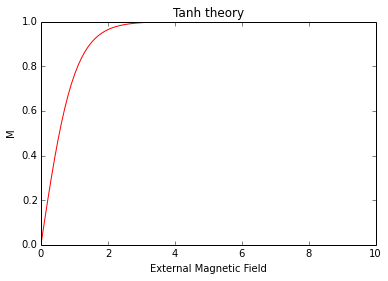
\includegraphics{display_2_0.png}

This is exactly the thing we saw in the experiment.

This can be classified as a category of problems. In this specific example we see saturation of magnetization. However this is not alway true.

\begin{notice}{note}{Note:}
Examples can be shown here.
\end{notice}


\subsubsection{Heat Capacity}
\label{equilibrium/week1:heat-capacity}
Another category of problems is temperature related. For example, a study of average energy with change temperature.

For the paramagnetic example, the energy of the system is
\begin{gather}
\begin{split}E = -(\mu B N e^{\beta \mu B} - \mu N e^{-\beta \mu B})/(\exp(\beta \mu B) + \exp(-\beta \mu B)) = -\mu N B \tanh (\beta \mu B)\end{split}\notag\\\begin{split}\end{split}\notag
\end{gather}
Obviously, no phase transition would occur. But if we introduce self interactions between dipoles and go to higher dimensions, it's possible to find phase transitions.


\subsubsection{Importance of Dimensions}
\label{equilibrium/week1:importance-of-dimensions}
\href{http://nbviewer.ipython.org/github/emptymalei/StatisticalPhysics/blob/master/equilibrium/homework/StatMech\_HW1.ipynb}{IPython Notebook about heat capacity of systems with different dimensions.} .


\subsection{Week 2}
\label{equilibrium/week2::doc}\label{equilibrium/week2:week-2}

\subsubsection{Behaviors of functions}
\label{equilibrium/week2:behaviors-of-functions}
(This part is synchronized to vocabulary chapter for future use.)
\begin{enumerate}
\item {} 
Tanh(x)

\end{enumerate}
\begin{figure}[htbp]
\centering
\capstart

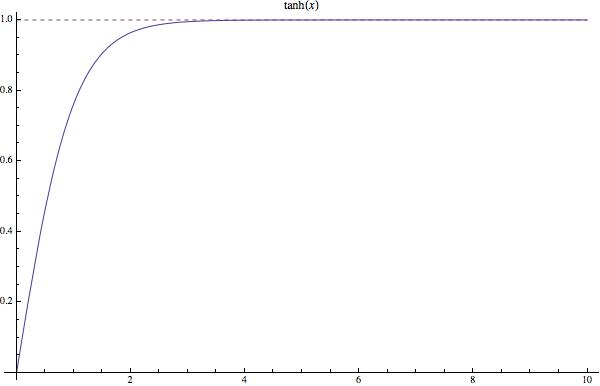
\includegraphics{tanh.jpg}
\caption{Tanh(x) from wolfram alpha}\end{figure}
\begin{enumerate}
\setcounter{enumi}{1}
\item {} 
$1-exp(-x)$

\end{enumerate}

{\hfill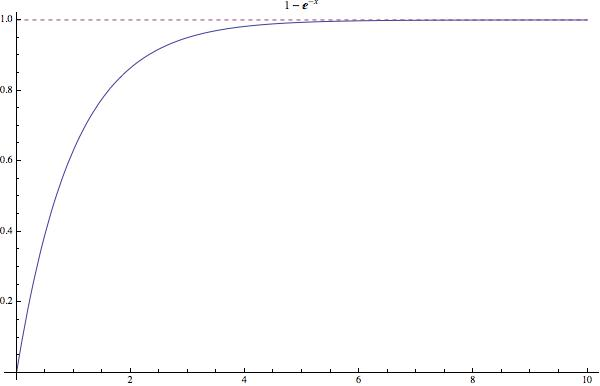
\includegraphics{exp1.jpg}\hfill}
\begin{enumerate}
\setcounter{enumi}{2}
\item {} 
$cosh(1/x)-1/x$

\end{enumerate}

{\hfill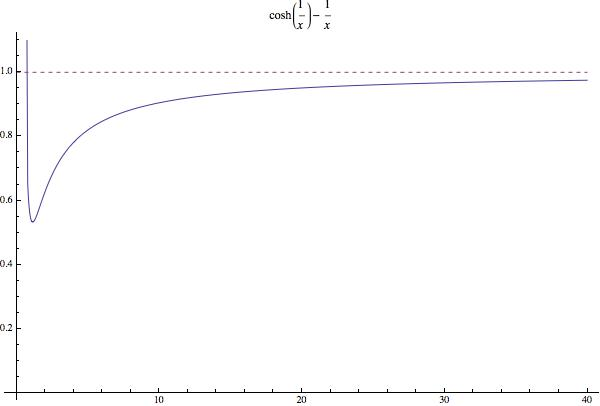
\includegraphics{cosh1.jpg}\hfill}
\begin{enumerate}
\setcounter{enumi}{3}
\item {} 
$1/(1+1/x)$

\end{enumerate}

{\hfill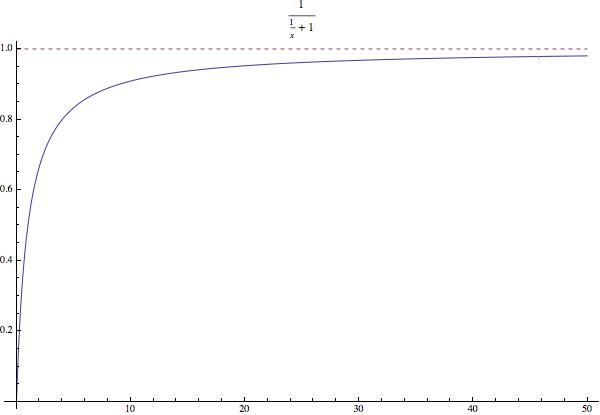
\includegraphics{fraction1.jpg}\hfill}

\begin{notice}{note}{Note:}
An example of this $1/(1+1/x)$ is the modified gas model.
\begin{gather}
\begin{split}P (V - b) = N k T\end{split}\notag\\\begin{split}\end{split}\notag
\end{gather}
We can find out $1/V$, which is
\begin{gather}
\begin{split}\frac{1}{V} = \frac{1}{b+\frac{N k T}{P}}\end{split}\notag\\\begin{split}\end{split}\notag
\end{gather}
Now we can plot out $\frac{1}{V} ~ P$ and it shows a behavior just like $1/(1+1/x)$.
\end{notice}

\begin{notice}{note}{Note:}
To see the true nature of graphs, make quantities dimensionless. This is also true for theoretical derivations. Dimensionless equations can reveal more.
\end{notice}

Behavior of Boltzmann factor.

{\hfill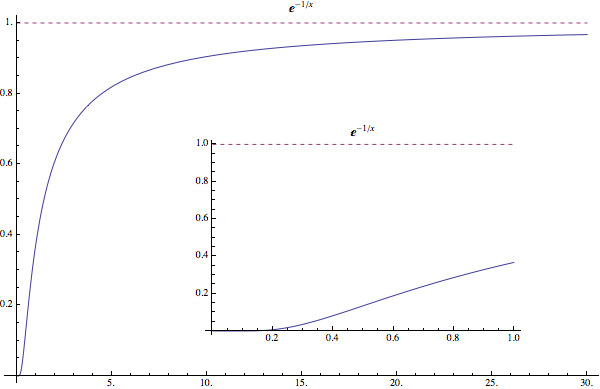
\includegraphics{boltzfactor.png}\hfill}

\begin{notice}{note}{Note:}
The nth derivative of this function is always 0 at x=0, for all finite n. Then how does it rise? The only thing I can say is that we are actually dealing with infinite n.

Professor Kenkre: sleeping lion
\end{notice}


\subsubsection{Specific Heat}
\label{equilibrium/week2:specific-heat}\begin{gather}
\begin{split}C = \frac{d}{T}\langle E \rangle\end{split}\notag\\\begin{split}\end{split}\notag
\end{gather}
Check the behavior of specific heat,
\begin{enumerate}
\item {} 
Is there a Discontinuity?

\item {} 
Constant?

\item {} 
Blow up?

\item {} 
Converge?

\end{enumerate}

Specific heat can be used for second order phase transition. An simple example of this is Landau theory.


\subsubsection{Partition Function}
\label{equilibrium/week2:partition-function}
For a given Hamiltonian H, the (classical) partition function Z is
\begin{gather}
\begin{split}Z = \int d q \int d x e^{-\beta H}\end{split}\notag\\\begin{split}\end{split}\notag
\end{gather}
A simple example is the Harmonic Oscillator,
\begin{gather}
\begin{split}H = \frac{p^2}{2m} + \frac{1}{2} q x^2\end{split}\notag\\\begin{split}\end{split}\notag
\end{gather}
The partition function
\begin{gather}
\begin{split}Z = \int e^{-\beta p^2/(2m)} d q \int  e^{-\beta \frac{1}{2} q x^2 } d x  = 2\pi \sqrt{m/q} \frac{1}{\beta}\end{split}\notag\\\begin{split}\end{split}\notag
\end{gather}
Energy
\begin{gather}
\begin{split}E = \frac{1}{Z} \int \int e^{-\beta p^2/(2m)}   e^{-\beta \frac{1}{2} q x^2 }  H d p d x  = \cdots = k_B T\end{split}\notag\\\begin{split}\end{split}\notag
\end{gather}
(This result is obvious if we think about equipartition theorem.)

A more clever approach for the energy is to take the derivative of partition function over $\beta$, which exactly is
\begin{gather}
\begin{split}\langle E \rangle = -\frac{\partial }{\partial \beta } \ln Z\end{split}\notag\\\begin{split}\end{split}\notag
\end{gather}
In our simple case,
\begin{gather}
\begin{split}\ln Z = -\frac{\partial}{\partial \beta} \left(\ln (k_B T) + \mathrm{Some Constant} \right)= k_B T\end{split}\notag\\\begin{split}\end{split}\notag
\end{gather}
This is the power of partition function. To continue the SHO example, we find the specific heat is
\begin{gather}
\begin{split}C = k_B\end{split}\notag\\\begin{split}\end{split}\notag
\end{gather}
\begin{notice}{note}{Note:}
This result has nothing to do with the detail of the SHO, no matter what mass they have, no matter what potential constant $q$ they have, no matter what kind of initial state they have. All the characteristic quantities of SHO are irrelevant. Why? Mathematically, it's because we have Gaussian integral here. \textbf{But what is the physics behind this?} Basicly this classical limit is a high temperature limit.
\end{notice}


\subsubsection{Quantum Harmonic Oscillator}
\label{equilibrium/week2:quantum-harmonic-oscillator}
Quantum HO tells us the eigen energy
\begin{gather}
\begin{split}E_n  = \left(n + \frac{1}{2}\right)\hbar \omega\end{split}\notag\\\begin{split}\end{split}\notag
\end{gather}
where $\omega = \sqrt{ k/m }$.

Partition function
\begin{gather}
\begin{split}Z = \sum_n e^{-\beta E_n} = \frac{e^{-\frac{1}{2} \hbar \omega }} { 1 - e^{- \beta \hbar \omega} } = \frac{1}{2}  \sinh(\beta \hbar \omega/2)\end{split}\notag\\\begin{split}\end{split}\notag
\end{gather}
Energy
\begin{gather}
\begin{split}\langle E \rangle = -\frac{\partial}{\partial\beta} \ln Z =  \hbar \omega \left( \frac{1}{2} + \frac{1}{\exp(\beta\hbar\omega) - 1} \right)\end{split}\notag\\\begin{split}\end{split}\notag
\end{gather}
Specific heat
\begin{gather}
\begin{split}C = \frac{\partial}{\partial T} \langle E\rangle = k_B (\beta \hbar \omega)^2 \frac{\exp(\beta \hbar \omega)}{ (\exp(\beta \hbar \omega) - 1)^2 }\end{split}\notag\\\begin{split}\end{split}\notag
\end{gather}
This specific heat behaves like this.

{\hfill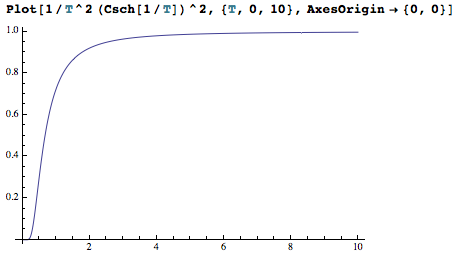
\includegraphics{shQHO.png}\hfill}

Though we have infinite energy levels, the specific heat won't blow up because the probability of a high energy level state is very small.


\subsubsection{Density of States}
\label{equilibrium/week2:density-of-states}
\begin{notice}{note}{Note:}
Free energy
\begin{gather}
\begin{split}A = U - T S\end{split}\notag\\\begin{split}\end{split}\notag
\end{gather}
In another way,
\begin{gather}
\begin{split}A = - k_B T \ln Z\end{split}\notag\\\begin{split}\end{split}\notag
\end{gather}
As long as we find out partition function, all thermodynamics quantities are solved, including entropy.
\begin{gather}
\begin{split}S = -k_B \beta  \left(T \ln Z - \frac{\partial}{\partial \beta} \ln Z \right)\end{split}\notag\\\begin{split}\end{split}\notag
\end{gather}\end{notice}

Specific heat is very different in 1D, 2D, 3D even for similar Hamiltonian. In the case of dipole systems, this is because for 1D, there discrete energy levels, for 2D and 3D energy levels fill up the gap. But what's the difference between 2D and 3D? Obviously the degeneracies are different.

Generally,
\begin{gather}
\begin{split}Z = \int g(E) e^{-\beta E}\mathrm d E\end{split}\notag\\\begin{split}\end{split}\notag
\end{gather}
where $g(E)$ is the density of states.


\paragraph{Calculation of DoS}
\label{equilibrium/week2:calculation-of-dos}
QM free particle in a 2D box.

In the momentum (wave number) space, all possible states are distributed on a grid.

{\hfill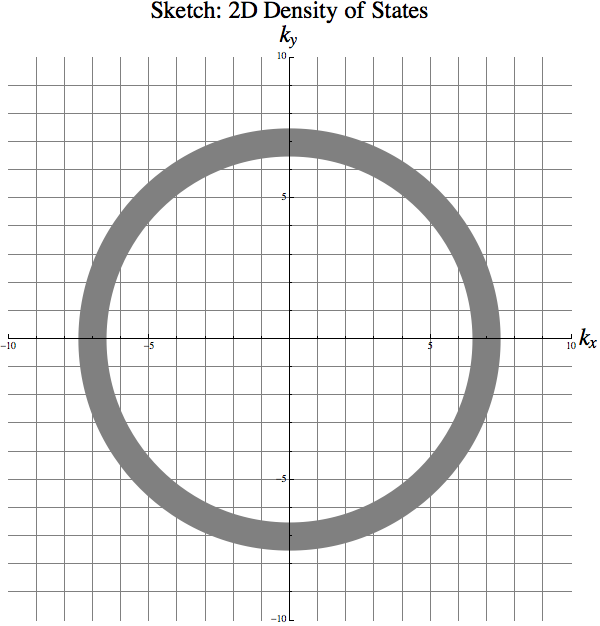
\includegraphics{2DDos.png}\hfill}

How do we calculate the DoS? For a given E, we have $k_x^2 + k_y^2 = \mathrm{Constant} E$. The \# of states between $E ~ E + \mathrm d E$ is just the area of it divided by the area of each grid box.
\begin{gather}
\begin{split}N = \frac{d V_k}{d V_0} = \frac{2\pi k d k}{\frac{2\pi}{L_x} \frac{2\pi}{L_y} } \equiv g(E) d E\end{split}\notag\\\begin{split}\end{split}\notag
\end{gather}
DoS $g(E)$ is
\begin{gather}
\begin{split}g(E) = \frac{ 2\pi k }{\frac{d E}{d k}} \frac{L_x L_y}{(2\pi)^2}\end{split}\notag\\\begin{split}\end{split}\notag
\end{gather}
In the laguage of physics,
\begin{gather}
\begin{split}g(E) = \frac{\mathrm{area of } E ~ d E}{|\nabla_k E|} \frac{\mathrm{Volume of the box} }{(2\pi)^d}\end{split}\notag\\\begin{split}\end{split}\notag
\end{gather}
where $d$ is the dimension of the system or box.

Gradient of energy gives us the spread out or dispersion.

To sum up, the quantities that determines the DoS are,
\begin{itemize}
\item {} 
$E(k)$

\item {} 
$n$: dimension

\item {} 
$V$: volume of the box (important in QM because this sets the boundary conditions)

\end{itemize}


\paragraph{Examples of DoS}
\label{equilibrium/week2:examples-of-dos}\begin{enumerate}
\item {} 
2D free particle in a box with length $L$
\begin{gather}
\begin{split}\frac{d E}{d k} = \frac{d}{d k}\left( \frac{\hbar^2 k^2}{2m} \right) = \frac{\hbar^2 k}{m}\end{split}\notag\\\begin{split}\end{split}\notag
\end{gather}
Thus we have,
\begin{gather}
\begin{split}g(E) = \frac{2\pi k }{\frac{\hbar^2 k}{m}} \frac{L^2}{(2\pi)^2} = (\frac{1}{2\pi} \frac{m}{\hbar^2})L^2\end{split}\notag\\\begin{split}\end{split}\notag
\end{gather}
\item {} 
3D free particle in a box with length $L$
\begin{gather}
\begin{split}\frac{d E}{d k} = \frac{\hbar^2 k^2}{2m}\end{split}\notag\\\begin{split}\end{split}\notag
\end{gather}
DoS
\begin{gather}
\begin{split}g(E) = \frac{m}{\hbar^2} \frac{L^3}{2\pi^2} k\end{split}\notag\\\begin{split}\end{split}\notag
\end{gather}
This is $k$ dependent.

\item {} 
1D
\begin{gather}
\begin{split}g(E) = \frac{1}{k} \frac{m L}{2\pi \hbar^2}\end{split}\notag\\\begin{split}\end{split}\notag
\end{gather}
\end{enumerate}

\begin{notice}{note}{Note:}
These results are so different. For 1D system, the higher energy of the system is, the small DoS is. 2D DoS doesn't depend on energy. 3D is proportional to the square root of energy.

DoS is very important in quantum systems because quantization can make strange DoS. In classical systems without quantization, DoS is always some kind of constant.
\end{notice}


\subsubsection{Partition Function and DoS}
\label{equilibrium/week2:partition-function-and-dos}
Thermal wavelength is defined as
\begin{gather}
\begin{split}\lambda_T = \frac{\hbar}{ \sqrt{ 2\pi m k_B T } }\end{split}\notag\\\begin{split}\end{split}\notag
\end{gather}
For 1 particle in 3D box,
\begin{gather}
\begin{split}Z_1 = \frac{V}{\lambda_T^3}\end{split}\notag\\\begin{split}\end{split}\notag
\end{gather}
It's obvious that for a N particles system without interaction between particles, $Z_N  = (Z_1)^N$. Free energy
\begin{gather}
\begin{split}A = -k_B T \ln (Z_N) = -k_B T N \ln Z_1 = -k_B T N (\ln V - 3\ln \lambda_T)\end{split}\notag\\\begin{split}\end{split}\notag
\end{gather}
\begin{notice}{note}{Note:}
This quantity is neither intensive nor extensive! If we combine two exactly same system, then we won't have twice of the free energy. It's called Gibbs mixing paradox.
\end{notice}


\subsection{Week 3}
\label{equilibrium/week3::doc}\label{equilibrium/week3:week-3}

\subsubsection{Phase Space of Quantum Partition Function}
\label{equilibrium/week3:phase-space-of-quantum-partition-function}
This is a physical idea of how do we get the quantum partition function from Classical Mechanics.

Classically, the partition function
\begin{gather}
\begin{split}Z = \int d^3 x \int d^3 p e^{-\beta p^2/2m} = V \left( \sqrt{\frac{ 2m \pi }{\beta} } \right)^3\end{split}\notag\\\begin{split}\end{split}\notag
\end{gather}
We can see from this that thermal wave length is $1/\sqrt{\frac{ 2m \pi }{\beta}}$ classically. In quantum, partition function is a summation,
\begin{gather}
\begin{split}Z = \sum_i e^{-\beta E_i}\end{split}\notag\\\begin{split}\end{split}\notag
\end{gather}
If we are going to write this into some integration, which is something like
\begin{gather}
\begin{split}Z = \int d^3 x\int d^3 p e^{ -\beta p^2/2m }\end{split}\notag\\\begin{split}\end{split}\notag
\end{gather}
which is problematic because it has a different dimension with the summation definition. So we need to put some quantity which has a dimension $[p\cdot x ]^3$, and it got to be $h^3$. So the integration form of partition function is
\begin{gather}
\begin{split}Z = \frac{1}{h^3} \int d^3 x\int d^3 p e^{ -\beta p^2/2m }\end{split}\notag\\\begin{split}\end{split}\notag
\end{gather}
\begin{notice}{note}{Note:}
$h^3$ is the smallest phase space volume in quantum mechanics.
\end{notice}

\begin{notice}{warning}{Warning:}
Here we used phase space of ${q_i;p_i}$ which is not a good choice for quantum mechanics. So this might be a problem. Should check books for a more rigorous method.
\end{notice}


\subsubsection{Observables \& Equilibrium}
\label{equilibrium/week3:observables-equilibrium}
Average of an observable is
\begin{gather}
\begin{split}O = Tr(\hat O \rho)\end{split}\notag\\\begin{split}\end{split}\notag
\end{gather}
where $\rho$ is the ``probability matrix''. In QM, this is
\begin{gather}
\begin{split}\rho = \frac{ e^{-\beta H} }{\mathrm{Tr} ( e^{-\beta H} ) }\end{split}\notag\\\begin{split}\end{split}\notag
\end{gather}
If a system of QM comes to equilibrium, that means
\begin{enumerate}
\item {} 
$\rho  = \frac{ e^{-\beta H} }{\mathrm{Tr} e^{-\beta H} }$;

\item {} 
$\rho$ is diagonal in energy eigen space.

\end{enumerate}


\subsubsection{Gibbs Mixing Paradox}
\label{equilibrium/week3:gibbs-mixing-paradox}
As we already know, from math of classical statistical mechanics, free energy
\begin{gather}
\begin{split}A  = -k_B T N ( \ln V - 3 \ln \lambda )\end{split}\notag\\\begin{split}\end{split}\notag
\end{gather}
Suppose we have two systems, one with $N_1$ and $V_1$ the other with $N_2$ and $V_2$. Now we mix them. Our physics intuition would tell us that the free energy of this new system should be $A = A_1 + A_2$. However, from the free energy equation, we get
\begin{gather}
\begin{split}A = \cdots - k_B T \ln (V_1^{N_1} V_2^{N2})\end{split}\notag\\\begin{split}\end{split}\notag
\end{gather}
This is different from the result we thought of
\begin{gather}
\begin{split}A = \cdots - k_B T (N_1 + N_2) \ln (V_1 + V_2) = \cdots - k_B T \ln \left(  (V_1 + V_2)^{N_1+N_2}  \right)\end{split}\notag\\\begin{split}\end{split}\notag
\end{gather}
That is, free energy becomes neither intensive nor extensive in our derivation.

The fairly simple way to make it extensive is to \textbf{divide V by N}. Now a new term will appear in our free energy, namely $N\ln N$. Recall that in Sterling approximation, $\ln N! = N\ln N -N$. So in a large system, we can create some kind of free energy definition which makes it extensive.

\begin{notice}{note}{Note:}
We can't just pull out some results from statistical mechanics and apply them to a small system composed of several particles. In stat mech we use a lot of approximations like Sterling approximation which is only valid when particle number is huge.
\end{notice}
\begin{gather}
\begin{split}A = - k_B T N ( \ln(V/N!) - 3 \ln \lambda)\end{split}\notag\\\begin{split}\end{split}\notag
\end{gather}
which is to say
\begin{gather}
\begin{split}Z_N = \frac{Z_1^N}{N!}\end{split}\notag\\\begin{split}\end{split}\notag
\end{gather}
This definition ``solves'' the Gibbs mixing paradox. The physics of this modification requires QM.


\subsubsection{Interacting Particles}
\label{equilibrium/week3:interacting-particles}
Statistical mechanics starts from a given energy spectrum. With energy spectrum solved, we can do statistics.

For an interacting system, we need to solve the energy spectrum first then calculate the partition function. Usually we would have coupled equations for interacting systems. For example, in a coupled HO system with N oscillators. Image of two HO example is given here.

{\hfill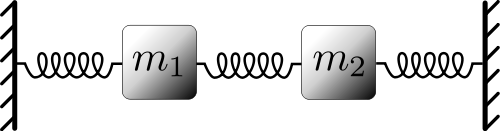
\includegraphics{Coupled_Harmonic_Oscillator.png}\hfill}

Our equations of motion are
\begin{gather}
\begin{split}m \ddot x_i + k( x_i -x_{i-1} + x_i - x_{i+1}) =0\end{split}\notag\\\begin{split}\end{split}\notag
\end{gather}
with i go from 2 to N-1.

A transformation $x_q = \sum x_m e^{i m q}$ will dissociate these equations,
\begin{gather}
\begin{split}m \ddot x_q + k' x_q =0\end{split}\notag\\\begin{split}\end{split}\notag
\end{gather}
We would have normal modes. $w_q ~ \sin|q/2|$.

In some sense, Debye theory is an many Einstein theory.
\begin{gather}
\begin{split}C_{\mathrm{Debye}} = \int C_{\mathrm{Einstein}} (\omega) g(\omega) d \omega\end{split}\notag\\\begin{split}\end{split}\notag
\end{gather}
In Einstein model, every particle is identical and have the same frequency. However, this theory shows a result of Boltzmann factor behavior, which is

{\hfill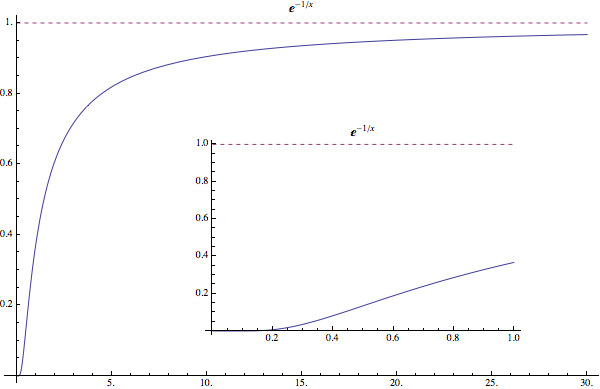
\includegraphics{boltzfactor.png}\hfill}

We got sleeping slope at very low temperature where experiments show that this wrong.

So the Debye theory is composed of two steps.
\begin{enumerate}
\item {} 
Calculate the energy spectrum of N coupled particle system by finding out a decouple transformation;

\item {} 
Evaluate the heat capacity integral.

\end{enumerate}

Once we find the energy spectrum, we will know the dispersion relation, which is different from Einstein's model.

{\hfill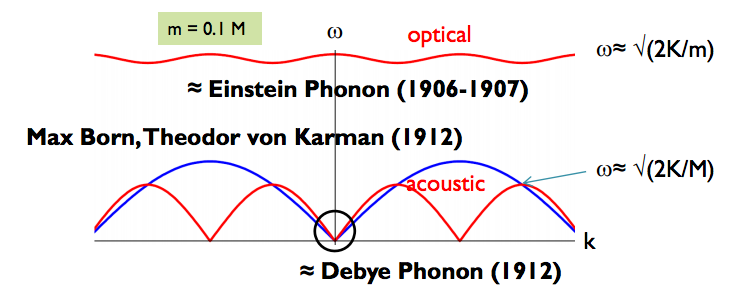
\includegraphics{DebyeModelkSpace.png}\hfill}

(Taken without permission from \href{http://griffin.ucsc.edu/teaching/08Q1-155/download/Lecture\%2006\%20-\%20Phonon\%20Dynamics.pdf}{here} .)

What did Debye do is to use a linear approximation, $w= c k$ for dispersion relation.

{\hfill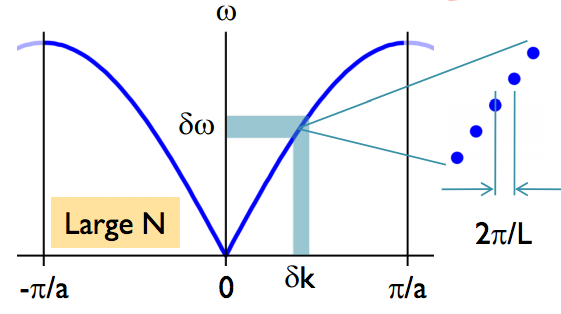
\includegraphics{DebyeModelApprox.png}\hfill}

(Taken without permission from \href{http://griffin.ucsc.edu/teaching/08Q1-155/download/Lecture\%2006\%20-\%20Phonon\%20Dynamics.pdf}{here} .)

Through a calculation, we show that
\begin{gather}
\begin{split}g(\omega) = \frac{V \omega^2}{2\pi^2 c^3}\end{split}\notag\\\begin{split}\end{split}\notag
\end{gather}
for a 3D lattice.

So average energy is
\begin{gather}
\begin{split}E = \frac{3V}{2\pi^2 c^3 \hbar^3} (k_B T)^4 \int_0^{x(\omega_m)} \frac{x^3}{e^x - 1} d x\end{split}\notag\\\begin{split}\end{split}\notag
\end{gather}
Heat Capacity is
\begin{gather}
\begin{split}C = 9 N k_B \left(\frac{T}{\Theta_D}\right)^3 \int _ 0 ^{x(\omega_m)} \frac{x^4 e^x}{(e^x - 1)^2} d x\end{split}\notag\\\begin{split}\end{split}\notag
\end{gather}
where $x(\omega_m) = \Theta_D/ T$ and $\Theta_D = \hbar \omega_D/k_B$.

\begin{notice}{note}{Note:}
What's amazing of Debye theory is that the low temperature behavior is independent of cut off frequency. At low temperature, $x(\omega_D)$ becomes infinite and it becomes an integration from 0 to infinity thus we do not need to know the cut off temperature to find out the low temperature result and it agrees with experiments well.
\end{notice}

\begin{notice}{important}{Important:}
We start for an Einstein theory and reaches a non sleeping model. What happened when we integrated over all DoS in Debye model? Work this out in details.

\begin{notice}{hint}{Hint:}
This has something to do with density of states dispersion relation.
\end{notice}

This is because our density of states $g(\omega)\propto \omega^2$ at low temperature tells us that we would have more states at a certain energy as $\omega$ increases. That is to say the system need more energy to increase temperature, identically the heat capacity line becomes steeper.
\end{notice}

\begin{notice}{important}{Important:}
Why is the \# of modes important in Debye model? The degree of freedom is finite in an system. If we don't cut off the frequency, that means we would have infinite degree of freedom because we have made an approximation that dispersion relation is a straight line $\omega = c k$. That would certainly lead to infinite heat capacity and infinite total energy.
\end{notice}


\subsubsection{Beyond Debye Model}
\label{equilibrium/week3:beyond-debye-model}
Debye model is simple yet classic. Generally we can not find the right transformation that decouples the particles. For example we have the Ising model,
\begin{gather}
\begin{split}H = \sum_i \mu \sigma B - \sum _ {i,j} J^{ij}\sigma_i \sigma _ j\end{split}\notag\\\begin{split}\end{split}\notag
\end{gather}
with $J^{ij} = J (  \delta _ i \delta _ {j-1} +\delta _ i \delta _{j+1} )$ as an simple model.

\begin{notice}{hint}{Hint:}
The reason that we can decouple the simple coupled HO system is that the coupling constant are the same and each HO is identical. In that case the system is just a homogeneous chain such that the normal modes are sin or cos waves depending on the boundary condition. If the system is inhomogeneous, there is no way that we can use simple plain waves on the chain as normal modes.
\end{notice}


\subsection{Week 4}
\label{equilibrium/week4:week-4}\label{equilibrium/week4::doc}

\subsubsection{Phase Transitions}
\label{equilibrium/week4:phase-transitions}
a link \href{http://jfi.uchicago.edu/~leop/TALKS/Perimeter\%20Stat\%20Mech\%20Lectures/lectures\%20in\%20PDF/Part\%207\%20Mean\%20Field\%20Theory.pdf}{here}.

Phase transitions are a property of infinite systems.


\subsubsection{Mean Field Thoery}
\label{equilibrium/week4:mean-field-thoery}
More is the same.

\begin{notice}{note}{Note:}
Why is this an approximation?
Because the actual magnetic field for example is often not the average of all the magnetic dipoles.
\end{notice}

Mean field theory often fails at the critical points that is mean field theory is not precise enough for phase transition in some low dimensional systems. This gives us a very interesting thought.

\begin{notice}{important}{Important:}
Why does mean field theory work? From the view of mathematics, potential can always be expanded at some value which is exactly the mean value of the field. For an Hamiltonian,
\begin{gather}
\begin{split}H = - \sum _{\langle i,j \rangle} J^{ij} \sigma_i \sigma_j - \mu \sum_i h^i \sigma_i\end{split}\notag\\\begin{split}\end{split}\notag
\end{gather}
Mean field treatment is
\begin{gather}
\begin{split}H = - \sum _{\langle i,j \rangle} J^{ij} \sigma_i \sigma - \mu \sum_i h^i \sigma_i\end{split}\notag\\\begin{split}\end{split}\notag
\end{gather}
where $\sigma = \sum_i \sigma_i/N$ is the average spin configuration.

This looks just like we take the 0 order of spin configuration expansion. And we can also include the second order which means add the interaction of just two spins.
\end{notice}

\begin{notice}{note}{Note:}
Susceptibility is a parameter that shows how much an extensive parameter changes when an intensive parameter increases. Magnetic susceptibility is
\begin{gather}
\begin{split}\chi(T)= \frac{\mathrm d M(T)}{\mathrm T}\end{split}\notag\\\begin{split}\end{split}\notag
\end{gather}\end{notice}

\begin{notice}{important}{Important:}
What makes the phase transition in such a system? Finite system has no phase transitions because finite continuous function can only make up continuous function by addition. Phase transition happens when the correlation length becomes infinite. So this is all about correlations.
\end{notice}

\begin{notice}{important}{Important:}
Why is mean field theory an approximation? Because the actual spin is more or less different from the average of spin configuration. Fluctuations in the spin makes the difference.
\end{notice}


\subsubsection{Gas Models}
\label{equilibrium/week4:gas-models}
Ideal gas is the simplest. Van de Waals model considers the correction in pressure and volume.
\begin{gather}
\begin{split}(P + a n^2/V^2)(V- n b) = n R T\end{split}\notag\\\begin{split}\end{split}\notag
\end{gather}
for n mole gas.
\begin{enumerate}
\item {} 
$nb$ is because molecules are not point particles, they take up space. In Lenard-Jones potential model, b is 4 times the size of all molecules.

\item {} 
$a n^2/V^2$ is because in this model molecules will attract to each other when they get too close. This attractive force makes it possible to have phase transition, condensation of gas molecules.

\end{enumerate}

This models, is basically a kind of mean field theory which treats the corrections as a mean field. More specifically, we write the original Hamiltonian
\begin{gather}
\begin{split}H = \sum \frac{\vec p_i^2}{2m} + \sum _ {\langle i,j \rangle} \phi(r_{ij})\end{split}\notag\\\begin{split}\end{split}\notag
\end{gather}
as
\begin{gather}
\begin{split}H = \sum \frac{\vec p_i^2}{2m} +  \sum _ {\langle i,j \rangle} \phi(r)\end{split}\notag\\\begin{split}\end{split}\notag
\end{gather}
in which $\phi(r)$ is the average of potential and all particles interaction have the same value.

Onnes used series to write the equation of state,
\begin{gather}
\begin{split}P = \frac{n R T}{V} \left[ 1 + \frac{n}{V} B(T) + \left(\frac{n}{V}\right)^2 C(T) + \cdots \right]\end{split}\notag\\\begin{split}\end{split}\notag
\end{gather}
This can be derived using Mayer function and cluster expansion.


\subsubsection{Ensemble}
\label{equilibrium/week4:ensemble}
A standard procedure of solving mechanics problems, said by Prof. Kenkre which is don't really accept, is

Initial condition / Description of states -\textgreater{} Time evolution -\textgreater{} Extraction of observables


\paragraph{States}
\label{equilibrium/week4:states}
\textbf{Density of states in phase space}

Continuity equation
\begin{gather}
\begin{split}\partial _ t \rho + \nabla \cdot (\rho \vec u) =0\end{split}\notag\\\begin{split}\end{split}\notag
\end{gather}
This conservation law can be more simpler if dropped the term $\nabla\cdot \vec u = 0$ for incompressibility.

Or more generally,
\begin{gather}
\begin{split}\partial _ t \rho + \nabla \cdot \vec j = 0\end{split}\notag\\\begin{split}\end{split}\notag
\end{gather}
and here $\vec j$ can take other definitions like $\vec j = - D \partial_x \rho$.

This second continuity equation can represent any conservation law provided the proper $\vec j$.

\begin{notice}{important}{Important:}
From continuity equation to Liouville theorem:

We start from
\begin{gather}
\begin{split}\frac{\partial}{\partial t} \rho + \vec \nabla \cdot (\rho \vec v)\end{split}\notag\\\begin{split}\end{split}\notag
\end{gather}
Divergence means
\begin{gather}
\begin{split}\vec \nabla \cdot  = \sum_i \left( \frac{\partial}{\partial q_i} + \frac{\partial}{\partial p_i} \right) .\end{split}\notag\\\begin{split}\end{split}\notag
\end{gather}
Then we will have the initial expression written as
\begin{gather}
\begin{split}\frac{\partial}{\partial t} \rho + \sum_i \left( \frac{\partial}{\partial q_i} (\rho \dot q_i) + \frac{\partial}{\partial \dot p_i} \right) .\end{split}\notag\\\begin{split}\end{split}\notag
\end{gather}
Expand the derivatives,
\begin{gather}
\begin{split}\frac{\partial}{\partial t} \rho + \sum_i \left[  \left( \frac{\partial}{\partial q_i} \dot q_i + \frac{\partial}{\partial p_i} \dot p_i\right) \rho +  \dot q_i \frac{\partial}{\partial q_i} \rho  + \dot p_i \frac{\partial}{\partial p_i} \rho  \right]   .\end{split}\notag\\\begin{split}\end{split}\notag
\end{gather}
Recall that Hamiltonian equations
\begin{gather}
\begin{split}\dot q_i  = \frac{\partial H}{\partial p_i}\end{split}\notag\\\begin{split}\dot p_i = - \frac{\partial H}{\partial q_i}\end{split}\notag
\end{gather}
Then
\begin{gather}
\begin{split}\left( \frac{\partial}{\partial q_i} \dot q_i + \frac{\partial}{\partial p_i} \dot p_i\right) \rho  .\end{split}\notag\\\begin{split}\end{split}\notag
\end{gather}
Finally convective time derivative becomes zero because $\rho$ is not changing with time in a comoving frame like perfect fluid.
\begin{gather}
\begin{split}\frac{d}{d t} \rho \equiv  \frac{\partial}{\partial t}\rho + \sum_i \left[ \dot q_i \frac{\partial}{\partial q_i} \rho  + \dot p_i \frac{\partial}{\partial p_i} \rho \right] =0\end{split}\notag\\\begin{split}\end{split}\notag
\end{gather}\end{notice}


\paragraph{Time evolution}
\label{equilibrium/week4:time-evolution}
Apply Hamiltonian dynamics to this continuity equation, we can get
\begin{gather}
\begin{split}\partial_t \rho = \{H, \rho\}\end{split}\notag\\\begin{split}\end{split}\notag
\end{gather}
which is very similar to quantum density matrix operator
\begin{gather}
\begin{split}\mathrm i \hbar \partial_t \hat \rho = [ \hat H, \hat \rho ]\end{split}\notag\\\begin{split}\end{split}\notag
\end{gather}
That is to say, the time evolution is solved if we can find out the Poisson bracket of Hamiltonian and probability density.


\paragraph{Requirements for Liouville Density}
\label{equilibrium/week4:requirements-for-liouville-density}\begin{enumerate}
\item {} 
Liouville theorem;

\item {} 
Normalizable;

\begin{notice}{hint}{Hint:}
What about a system with constant probability for each state all over the phase space? This is not normalizable. Such a system can not really pick out a value. It seems that the probability to be on states with a constant energy is zero. So no such system really exist. I guess?

Like this?

{\hfill\scalebox{0.900000}{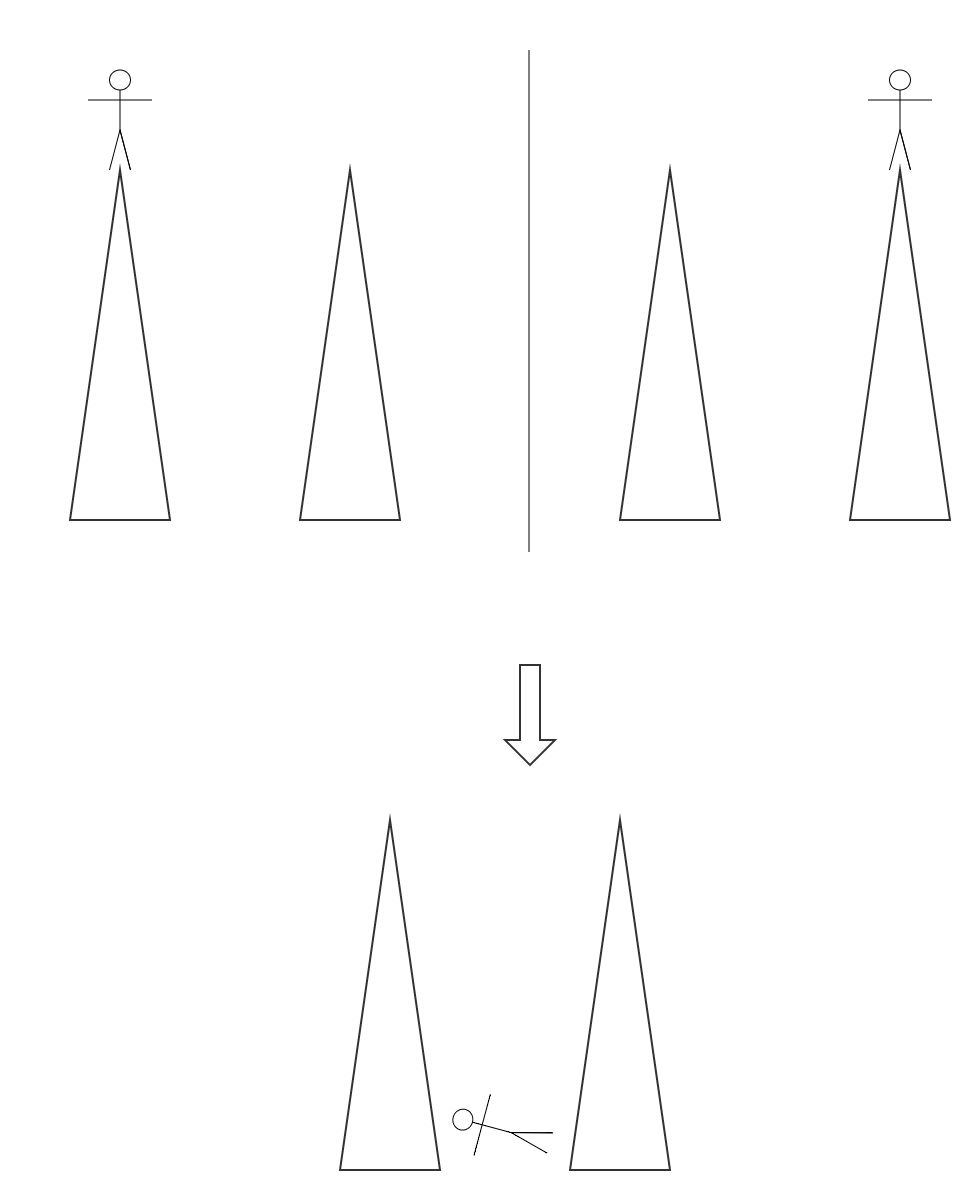
\includegraphics{sandiaPeaks.png}}\hfill}

Someone have 50\% probability each to stop on one of the two Sandia Peaks for a picnic. Can we do an average for such a system? \textbf{Example by Professor Kenkre.}
\end{notice}

\end{enumerate}

And one more for equilibrium systems, $\partial_t \rho =0$.


\paragraph{Extraction of observables}
\label{equilibrium/week4:extraction-of-observables}
It's simply done by using the ensemble average
\begin{gather}
\begin{split}\avg{O} = \int O(p_i; q_i;t) \rho(p_i;q_i;t) \sum_i dp_i dq_i dt\end{split}\notag\\\begin{split}\end{split}\notag
\end{gather}
where $i=1,2,..., 3N$.


\subsection{Week 5}
\label{equilibrium/week5:week-5}\label{equilibrium/week5::doc}
The problem in statistical mechanics is that we can only gain partial information of the system, thus only partial results are obtained. However we know that in equilibrium, all possible states appear with an equal probability. Recall that states means points in phase space. We use hydrodynamics to represent the phase space distribution but this can not determine if the phase space points are change or not. The only thing this density show us the the aparant density doesn't change. So it seems that we don't need to know the exact position of a phase space point. We can rely on average values.

The system is like a black box. Even we know all the quantities, we still have no idea about the exact state of the system.

\index{Ensemble}

\subsubsection{Ensemble}
\label{equilibrium/week5:index-0}\label{equilibrium/week5:ensemble}
Gibbs' idea of ensemble is to create a lot of copies of the system with the same thermodynamics quantities.

The question is where to put them? In different time or in different space?

We can create a uge amount copies of the system and imagine that they are at different place. Then we have all the possible states of the system.

We can also wait infinite long time and all possible states will occur, at least for some system, which is called ergodic. Ergodic means the system can visit all possible states many times during a long time. This is rather a hypothesis than a theorem.

The problem is, not all systems are ergodic. For such systems, of course, we can only do the ensemble average.

\begin{notice}{note}{Note:}
\textbf{Cons}
\begin{enumerate}
\item {} 
Not possible to prove ensemble average is the same as time average. In fact some systems don't obey this rule.

\item {} 
Not possible to visit all possible states on constant energy surface in finite time.

\item {} 
Even complicated systems can exhibit almost exactly periodic behavior, one example of this is \href{https://en.wikipedia.org/wiki/Fermi\%E2\%80\%93Pasta\%E2\%80\%93Ulam\_problem}{FPU experiment} .

\item {} 
Even the system is ergodic, how can we make sure each state will occur with the same probability.

\end{enumerate}

Here is an example of non ergodic system:

{\hfill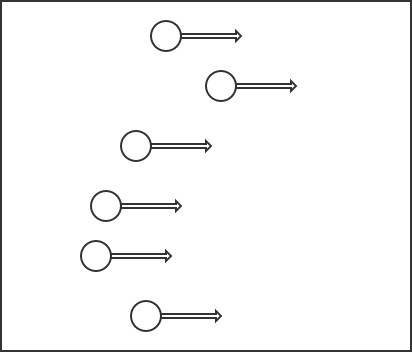
\includegraphics{non-ergodic.png}\hfill}

This is a box of absolutely smooth with balls collide with walls perpendicularly. Then this system can stay on some discrete points with same values of momentum components.

Another image from \href{https://commons.wikimedia.org/wiki/File:Ergodic\_hypothesis\_w\_reflecting\_rays.jpg}{Wikipedia} :

{\hfill\scalebox{0.900000}{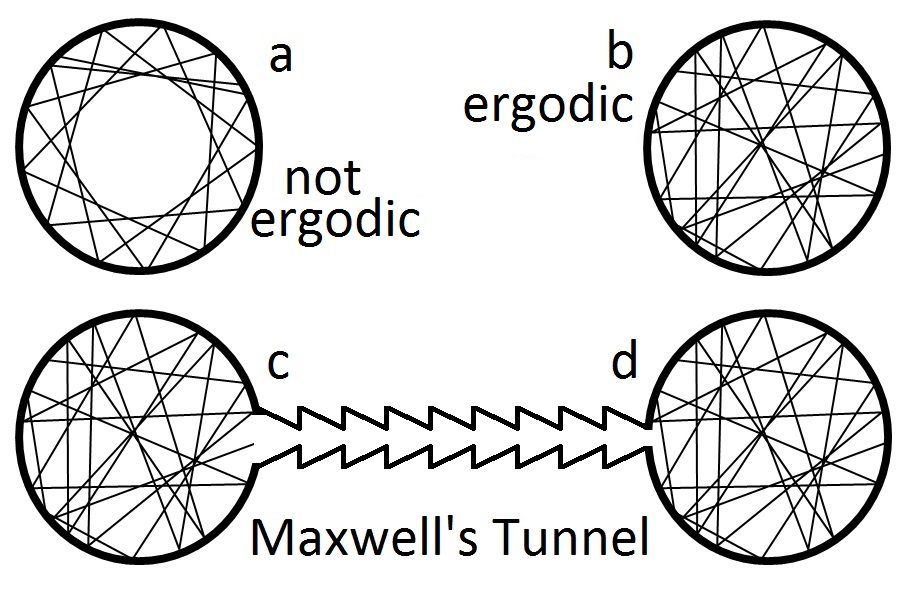
\includegraphics{Ergodic_hypothesis_w_reflecting_rays.jpg}}\hfill}
\end{notice}

\begin{notice}{note}{Note:}
\textbf{Pros}
\begin{enumerate}
\item {} 
\href{https://en.wikipedia.org/wiki/Poincar\%C3\%A9\_recurrence\_theorem}{Poincaré recurrence theorem} proves that at least some systems will come back to a state that is very close the the initial state after a long but finite time.

\item {} 
Systems are often chaotic so it's not really possible to have pictures like the first one in Cons.

\end{enumerate}
\end{notice}

We already have Liouville density evolution
\begin{gather}
\begin{split}\frac{\partial}{\partial t} \rho = \{ H, \rho \}\end{split}\notag\\\begin{split}\end{split}\notag
\end{gather}
Von Neumann equation
\begin{gather}
\begin{split}i\hbar \frac{\partial}{\partial t} \hat\rho = [\hat H, \hat\rho ]\end{split}\notag\\\begin{split}\end{split}\notag
\end{gather}
In all, they can be written as
\begin{gather}
\begin{split}i \frac{\partial\rho}{\partial t} = \hat L \rho\end{split}\notag\\\begin{split}\end{split}\notag
\end{gather}
where $\hat L$ is the Liouville operator.

We have mentioned that ensembles have the same thermodynamic quantities. In the language of math,
\begin{gather}
\begin{split}\avg{o} = \mathrm{Tr} \rho O\end{split}\notag\\\begin{split}\end{split}\notag
\end{gather}
All we care about is the left hand side. So as long as $\rho$ is not changed, we can stir the system as crazy as we can and keep the system the same.

\begin{notice}{hint}{Hint:}
Only one trace in phase space is true. How can we use ensemble to calculate the real observables?

Actually, what we calculated is not the real observable. What we calculated is the ensemble average. Since we are dealing with equilibrium, we need the time average because for equilibrium system, time average is the desired result. (Fluctuations? yes but later.) As we discussed previously, for ergodic systems, ensemble average is the same as time average.
\end{notice}


\subsubsection{Equilibrium}
\label{equilibrium/week5:equilibrium}
What does equilibrium mean exactly?
\begin{gather}
\begin{split}\frac{\partial}{\partial} \rho  = 0\end{split}\notag\\\begin{split}\end{split}\notag
\end{gather}
or equivalently,
\begin{gather}
\begin{split}\{ H, \rho \} =0\end{split}\notag\\\begin{split}\end{split}\notag
\end{gather}
Obviously, one possible solution is
\begin{gather}
\begin{split}\rho \propto e^{-\beta H}\end{split}\notag\\\begin{split}\end{split}\notag
\end{gather}

\subsubsection{Ensembles, Systems}
\label{equilibrium/week5:ensembles-systems}

\begin{threeparttable}
\capstart\caption{Ensembles and systems}

\begin{tabulary}{\linewidth}{|L|L|L|L|}
\hline
\textsf{\relax 
Systems
} & \textsf{\relax 
Ensembles
} & \textsf{\relax 
Geometry in Phase space
} & \textsf{\relax 
Key Variables
}\\
\hline
Isolated
 & 
Microcanonical
 & 
Shell; $\rho = c'\delta(E-H)$
 & 
Energy $E$
\\

Weak interacting
 & 
Canonical
 &  & \\

Exchange particles
 & 
Grand canonical
 &  & \\
\hline\end{tabulary}

\end{threeparttable}


\index{Microcanonical Ensemble}

\subsubsection{Isolated System - Micro-canonical Ensemble}
\label{equilibrium/week5:index-1}\label{equilibrium/week5:isolated-system-micro-canonical-ensemble}
{\hfill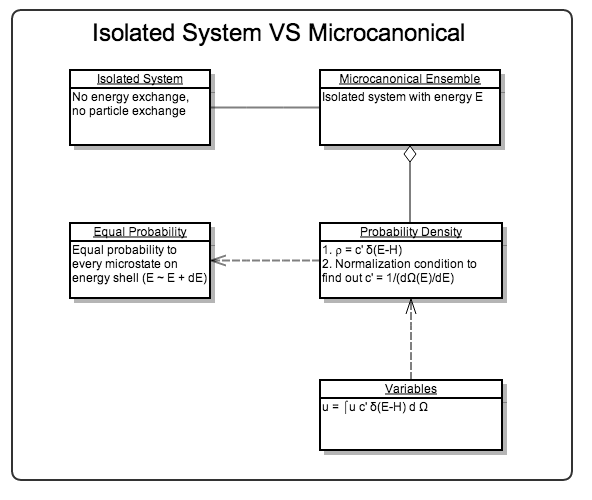
\includegraphics{microcanonical.png}\hfill}
\begin{gather}
\begin{split}\rho(p;q;0) = \delta(H(p;q;0) - E)\end{split}\notag\\\begin{split}\end{split}\notag
\end{gather}
That is the system stays on the energy shell in phase space. Also we have for equilibrium system,
\begin{gather}
\begin{split}H(p;q;t) = E\end{split}\notag\\\begin{split}\end{split}\notag
\end{gather}
\begin{notice}{hint}{Hint:}
Is it true that ensemble average is equal to the actual value of the system?

Not for all classical systems. (But for ALL quantum systems? Not sure.)
\end{notice}


\paragraph{Ergodic Hypothesis Revisited}
\label{equilibrium/week5:ergodic-hypothesis-revisited}
For ergodic systems, ensemble average is equal to time average.

\begin{notice}{important}{Important:}
How about state of the system moving with changing speed on the shell? Then how can we say the system is ergodic and use ensemble average as time average?
\end{notice}

Micro canonical ensembles are for isolated systems.
\begin{gather}
\begin{split}\rho \propto \frac{1}{\text{No. of states on the ensemble surface}} \equiv \frac{1}{\Omega (E)}\end{split}\notag\\\begin{split}\end{split}\notag
\end{gather}
To calculate the entropy
\begin{gather}
\begin{split}S = k_B \ln \Omega\end{split}\notag\\\begin{split}\end{split}\notag
\end{gather}
\index{Canonical Ensemble}

\subsubsection{Canonical Ensemble}
\label{equilibrium/week5:canonical-ensemble}\label{equilibrium/week5:index-2}
{\hfill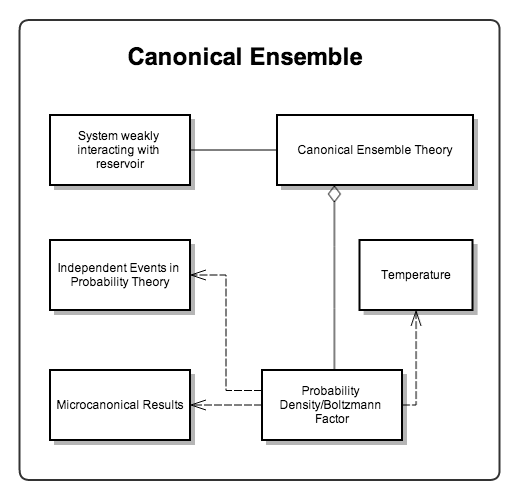
\includegraphics{canonicalEnsemble.png}\hfill}

For a system weakly interacting with a heat bath, total energy of the system is
\begin{gather}
\begin{split}E_T = E_S + E_R + E _{S,R}\end{split}\notag\\\begin{split}\end{split}\notag
\end{gather}
where the interacting energy $E$ is very small compared to $E_1\ll E_2$. So we can drop this interaction energy term,
\begin{gather}
\begin{split}E_T = E_S + E _R\end{split}\notag\\\begin{split}\end{split}\notag
\end{gather}
A simple and intuitive derivation of the probability density is to use the theory of independent events.
\begin{enumerate}
\item {} 
$\rho_T d\Omega_T$: probability of states in phase space volume $d\Omega_T$;

\item {} 
$\rho_S d \Omega_S$: probability of states in phase space volume $d\Omega_S$;

\item {} 
$\rho_R d \Omega_R$: probability of states in phase space volume $d\Omega_R$;

\end{enumerate}

We assumed weak interactions between system and reservoir, so (approximately) the probability in system phase space and in reservoir phase space are independent of each other,
\begin{gather}
\begin{split}\rho _ T d\Omega_T = \rho _S d\Omega_S \cdot \rho _R d \Omega_R .\end{split}\notag\\\begin{split}\end{split}\notag
\end{gather}
Since there is no particle exchange between the two systems, overall phase space volume is the system phase space volume multiplied by reservoir phase space volume,
\begin{gather}
\begin{split}d\Omega_T = d\Omega _S \cdot d\Omega_R .\end{split}\notag\\\begin{split}\end{split}\notag
\end{gather}
Obviously we can get the relation between the three probability densities.
\begin{gather}
\begin{split}\rho_T = \rho_R \rho_S .\end{split}\notag\\\begin{split}\end{split}\notag
\end{gather}
Take the logarithm,
\begin{gather}
\begin{split}\ln\rho_T = \ln\rho_R + \ln\rho_S .\end{split}\notag\\\begin{split}\end{split}\notag
\end{gather}
\textbf{Key: :math:{}`rho{}` is a function of energy :math:{}`E{}`. AND both :math:{}`rho{}` and energy are extensive. The only possible form of :math:{}`ln rho{}` is linear.}

Finally we reach the destination,
\begin{gather}
\begin{split}\ln \rho = - \alpha - \beta E\end{split}\notag\\\begin{split}\end{split}\notag
\end{gather}
i.e.,
\begin{gather}
\begin{split}\rho = e^{-\alpha} e^{-\beta E}\end{split}\notag\\\begin{split}\end{split}\notag
\end{gather}
which is called \textbf{canonical distribution}.

\begin{notice}{warning}{Warning:}
This is not an rigorous derivation. Read R.K. Su's book for a more detailed and rigorous derivation.
\end{notice}

\index{Grand Canonical Ensemble}

\subsubsection{Grand Canonical Ensemble}
\label{equilibrium/week5:grand-canonical-ensemble}\label{equilibrium/week5:index-3}
Systems with changing particle number are described by grand canonical ensemble.

{\hfill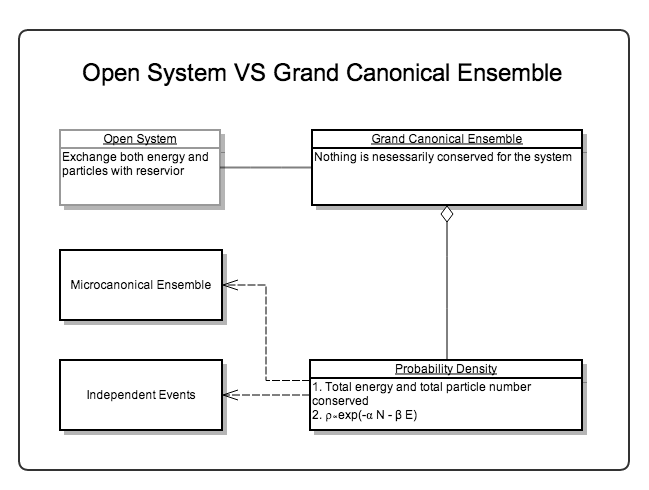
\includegraphics{grandCanonical.png}\hfill}

Note that the partition function of grand canonical ensemble really is
\begin{gather}
\begin{split}Z = \sum _ n \sum_N  e^{-\beta E_n - \mu N} = \sum_N \left( \sum _ n e^{- \beta E _ n}  \right)\left(e^{-\mu}\right)^N = \sum _ N Z \left(Z^f\right)^N\end{split}\notag\\\begin{split}\end{split}\notag
\end{gather}
\index{Identical Particles}

\subsubsection{Identical Particles}
\label{equilibrium/week5:index-4}\label{equilibrium/week5:identical-particles}
If a system consists of N indentical particles, for any state $n_i^\xi$ particles in particle state i, we have the energy of the system on state $\xi$ is
\begin{gather}
\begin{split}E^\xi = \sum_i \epsilon_i n_i^\xi\end{split}\notag\\\begin{split}\end{split}\notag
\end{gather}
where the summation is over all possible states of particles.

The value of energy is given by ensemble value
\begin{gather}
\begin{split}\avg{E} = \frac{\sum _\xi e^{-\beta E^\xi} E^\xi}{\sum _\xi e^{-\beta E^\xi}}\end{split}\notag\\\begin{split}\end{split}\notag
\end{gather}
$\xi$ is the ensemble summation.

\begin{notice}{hint}{Hint:}
How to calculate the average number of particles on a particle state i?
\end{notice}


\subsection{Week 6}
\label{equilibrium/week6:week-6}\label{equilibrium/week6::doc}

\subsubsection{Three Ensembles Cont'd}
\label{equilibrium/week6:three-ensembles-cont-d}
The three ensembles are the same when particle number N is really large, $N\rightarrow 0$ .

The reason is that
\begin{enumerate}
\item {} 
when N becomes really large, the interaction between system and reservoir becomes really negligible. The variance of Gaussian distribution is proportional to $1/\sqrt{N}$.

\item {} 
$dE_S+dE_R=dE$ and we know $dE=0$ so when the energy of the system increase that of reservoir drop. Professor Kenkre have a way to prove that the energy of the system is peaked at some value. However I didn't get it.

\end{enumerate}

\begin{notice}{warning}{Warning:}
Ask him why the value is peaked.
\end{notice}


\subsubsection{Most Probable Distribution}
\label{equilibrium/week6:most-probable-distribution}
Quite different from Gibbs' ensemble theory, Boltzmann's theory is about most probable distribution.
\begin{enumerate}
\item {} 
Classical distinguishable particles $a_l = w_l e^{-\alpha -\beta e_l}$;

\item {} 
Bosons $a_l = w_l \frac{1}{e^{\alpha+\beta e_l} - 1}$;

\item {} 
Fermion $a_l = w_l \frac{1}{e^{\alpha + \beta e_l} + 1}$.

\end{enumerate}

{\hfill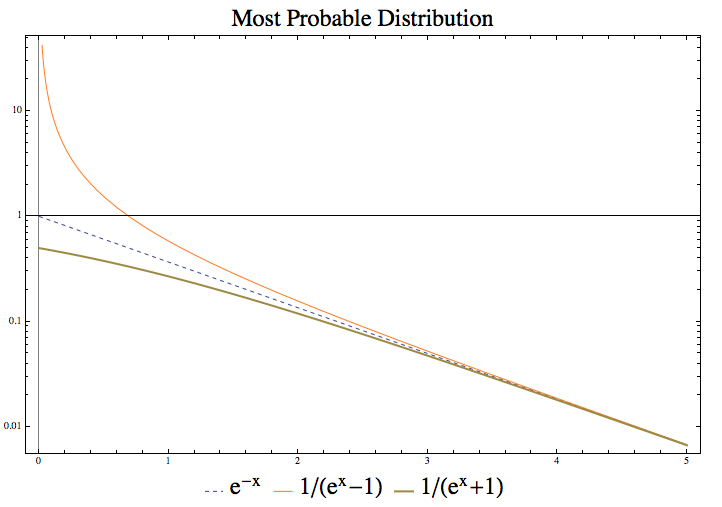
\includegraphics{mostProbableDistribution.png}\hfill}

This image tells us that the three lines converge when the factor $\alpha + \beta e_l$ becomes large. Also Fermions have less micro states than classical particles because of Pauli exclusive principle.

$\alpha + \beta e_l$ being large can have several different physical meanings.
\begin{enumerate}
\item {} 
Temperature low;

\item {} 
Energy high;

\item {} 
Chemical coupling coefficient $\alpha$ large.

\end{enumerate}

We have several identical conditions for the three distribution to be the same.
\begin{gather}
\begin{split}\alpha + \beta e_l \gg 1 \Leftrightarrow \alpha \gg 1 \Leftrightarrow 1/\exp(\alpha + \beta e_l) \ll 1 \Leftrightarrow a_l / w_l \ll 1\end{split}\notag\\\begin{split}\end{split}\notag
\end{gather}
where the last statement is quite interesting. $a_l/w_l \ll 1$ means we have much more states then particles and the quantum effects becomes very small.

\begin{notice}{warning}{Warning:}
One should be careful that even when the above conditions are satisfied, the number of micro states for classical particles is very different from quantum particles,
\begin{gather}
\begin{split}\Omega_{B.E} = \Omega_{F.D.} = \Omega_{M.B.}/N!  .\end{split}\notag\\\begin{split}\end{split}\notag
\end{gather}
This will have effects on entropy eventually.
\end{notice}

Recall that thermal wavelength $\lambda_t$ is a useful method of analyzing the quantum effect. At high temperature, thermal wavelength becomes small and the system is more classical.

\begin{notice}{hint}{Hint:}\begin{enumerate}
\item {} 
Massive particles $\lambda_t = \frac{h}{p} = \frac{h}{\sqrt{2m K}} = \frac{h}{\sqrt{ 2\pi m k T }}$

\item {} 
Massless particles $\lambda_t = \frac{c h}{2\pi^{1/3} k T}$

\end{enumerate}
\end{notice}

\textbf{However, at high temperature, the three micro states numbers are going to be very different. This is because thermal wavelength consider the movement of particles and high temperature means large momentum thus classical. The number of micro states comes from a discussion of occupation of states.}

\begin{notice}{important}{Important:}
What's the difference between ensemble probability density and most probable distribution? What makes the +1 or -1 in the occupation number?

Most probable distribution is the method used in Boltzmann's theory while ensemble probability density is in ensemble theory. That means in ensemble theory all copies (states) in a canonical ensemble appear with a probability density $\exp(-\beta E)$ and all information about the type of particles is in Hamiltonian.

Being different from ensemble theory, Boltzmann's theory deals with number of micro states which is affected by the type of particles. Suppose we have \emph{N} particles in a system and occupying $e_l$ energy levels with a number of $a_l$ particles. Note that we have a degeneration of $w_l$ on each energy levels.

{\hfill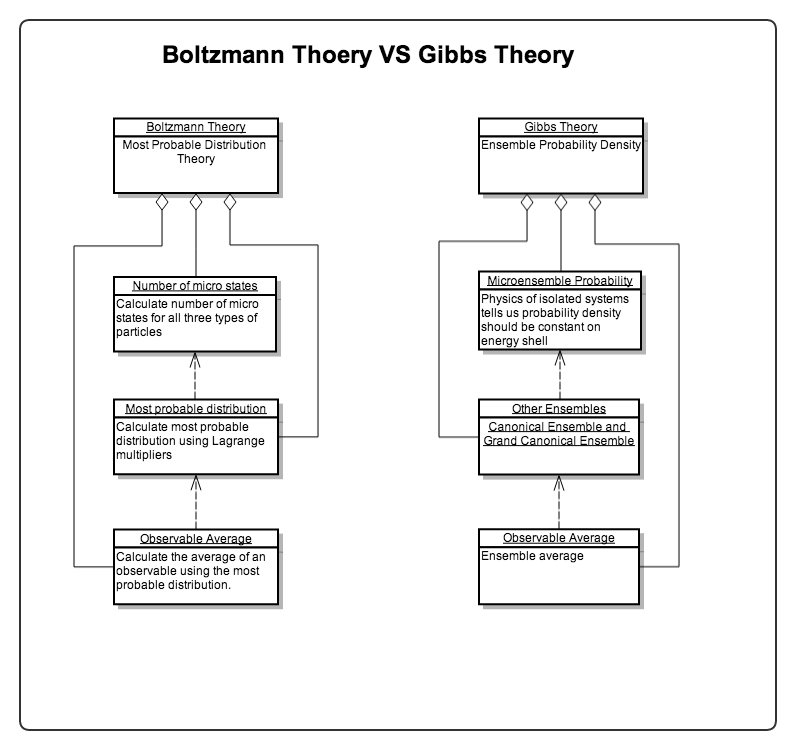
\includegraphics{BoltzmannVSGibbs.png}\hfill}

(Gliffy source here .)

For Boltzmann's theory, we need to
\begin{enumerate}
\item {} 
Calculate the number of micro states of the system;

\item {} 
Calculate most probable distribution using Lagrange multipliers;

\item {} 
Calculate the average of an observable using the most probable distribution.

\end{enumerate}

\begin{notice}{note}{Calculation of number of micro states}

Calculation of the number of micro states requires some basic knowledge of different types of particles.

For classical particles, we can distinguish each particle from others and no restrictions on the number of states on each energy level. Now we have $w_l^{a_l}$ possible states for each energy level. Since the particles are distinguishable we can have $N!$ possible ways of exchanging particles. But the degenerated particles won't contribute to the exchange (for they are the same and not distinguishable) which is calculated by $\Pi_l a_l!$.

Finally we have
\begin{gather}
\begin{split}\Omega _{M.B.} = \frac{N!}{\Pi_l a_l !} \Pi_l w_l^{a_l}\end{split}\notag\\\begin{split}\end{split}\notag
\end{gather}
as the number of possible states.

With similar techniques which is explicitly explained on Wang's book, we get the number of micro states for the other two types of particles.
\begin{gather}
\begin{split}\Omega _{B.E.} = \Pi_l \frac{(a_l+w_l-1)}{a_l!(w_l -1)!}\end{split}\notag\\\begin{split}\end{split}\notag
\end{gather}
is the number of micro states for a Boson system with a $\{a_l\}$ distribution.
\begin{gather}
\begin{split}\Omega _ {F.D.} = \Pi _ {l} C_{w_l}^{a_l} = \Pi _ l \frac{w_l!}{a_l!(w_l - a_l)!}\end{split}\notag\\\begin{split}\end{split}\notag
\end{gather}
is the number of micro states for a Fermion system with a distribution $\{a_l\}$. We get this because we just need to pick out $a_l$ states for $a_l$ particles on the energy level.
\end{notice}
\end{notice}


\subsubsection{The Exact Partition Function}
\label{equilibrium/week6:the-exact-partition-function}
DoS and partition function have already been discussed in previous notes.


\subsubsection{Is There A Gap Between Fermion and Boson?}
\label{equilibrium/week6:is-there-a-gap-between-fermion-and-boson}
Suppose we know only M.B. distribution, by applying this to harmonic oscillators we can find that
\begin{gather}
\begin{split}\avg{H} = (\bar n + 1/2)\hbar \omega\end{split}\notag\\\begin{split}\end{split}\notag
\end{gather}
where $\bar n$ is given by
\begin{gather}
\begin{split}\bar n = \frac{1}{e^{\beta \hbar \omega} - 1}\end{split}\notag\\\begin{split}\end{split}\notag
\end{gather}
which clearly indicates a new type of Boson particles.

So classical statistical mechanics and quantum statistical mechanics are closely connected not only in the most micro state numbers but also in a more fundamental way.

\begin{notice}{hint}{Hint:}
Note that this is possible because energy differences between energy levels are the same for arbitrary adjacent energy levels. Adding one new imagined particle with energy $\hbar\omega$ is equivalence to excite one particle to higher energy levels. So we can treat the imagined particle as a Boson particle.
\end{notice}


\chapter{Nonequilibrium System}
\label{index:nonequilibrium-system}
\index{Non-Equilibrium}

\section{Stochastic And Non-Equilibrium Statistical Mechanics}
\label{nonequilibrium/main:index-0}\label{nonequilibrium/main:stochastic-and-non-equilibrium-statistical-mechanics}\label{nonequilibrium/main::doc}
Stochastic process is very important in many fields of physics.

\index{nonequilibrium}

\subsection{Week 7}
\label{nonequilibrium/week7:index-0}\label{nonequilibrium/week7:week-7}\label{nonequilibrium/week7::doc}
\index{BBGKY}\index{Gamma Space}\index{mu Space}

\subsubsection{Two Spaces}
\label{nonequilibrium/week7:two-spaces}\label{nonequilibrium/week7:index-1}
To get some easy equations we need to reduce from $\Gamma$ space to $\mu$ space.

\begin{tabulary}{\linewidth}{|L|L|L|}
\hline
\textsf{\relax 
Two Spaces
} & \textsf{\relax 
$\Gamma$ space
} & \textsf{\relax 
$\mu$ space
}\\
\hline
Dimensions
 & 
$6 N$
 & 
$6$
\\

State of system
 & 
A point
 & 
$N$ points
\\

Probability density
 &  \multicolumn{2}{l|}{
$\rho(q^n_i, p^n_i; t)$                             \textbar{}  $f_n(q_i,p_i; t)$
}\\

Observables
 &  \multicolumn{2}{l|}{
Difference in the integration
}\\

EoM
 & 
Liouville equation or Von Neumann equation
 & 
BBGKY Hierarchy
\\
\hline\end{tabulary}



\subsection{Week 8}
\label{nonequilibrium/week8::doc}\label{nonequilibrium/week8:week-8}
\index{nonequilibrium}\index{BBGKY}\index{Liouville Operator}

\subsubsection{Liouville Operator And Liouville Equation}
\label{nonequilibrium/week8:index-0}\label{nonequilibrium/week8:liouville-operator-and-liouville-equation}
Instead of writing Poisson bracket as an bracket, we can define a Poisson bracket operator:
\begin{gather}
\begin{split}\hat{\mathscr H}^N = - \sum_{j=1}^N \left( \frac{\partial H^N}{\partial \vec q_j}\frac{\partial}{\partial \vec p_j} - \frac{\partial H^N}{\partial \vec p_j}\frac{\partial}{\partial \vec q_j} \right)\end{split}\notag\\\begin{split}\end{split}\notag
\end{gather}
More generally, we can define an Liouville operator, which is
\begin{gather}
\begin{split}\hat L^N := -i \hat{\mathscr H}^N  .\end{split}\notag\\\begin{split}\end{split}\notag
\end{gather}
Now the Liouville equation becomes
\begin{gather}
\begin{split}i \frac{\partial \rho^N}{\partial t} = \hat L^N \rho^N  .\end{split}\notag\\\begin{split}\end{split}\notag
\end{gather}
For stationary state we have
\begin{gather}
\begin{split}\hat L^N \rho^N _ {\mathrm{stationary}} = 0 .\end{split}\notag\\\begin{split}\end{split}\notag
\end{gather}

\subsubsection{BBGKY Hierarchy}
\label{nonequilibrium/week8:bbgky-hierarchy}
Now we think about the problems we are going to solve. In statistical mechanics, the most ideal method is to solve the Liouville equation directly and leave only initial condition missing for the problem. However, solving the Liouville equation is so hard for complicated problems we finally thinking about dropping some dynamics. This is no big deal as we already dropped initial condition and makes our solution probabilistic.

Now the question is what to drop. For non-interacting systems, the solution comes directly from Liouville equation. It's interactions that makes our life so hard (yet make us alive). So we would like to make approximations on interactions.

For non-interacting systems, $\Gamma$ space can actually be reduced to $\mu$ space which is spanned by the freedoms of only one particle. Here we need to address the fact that we are dealing with \textbf{identical particles}.

Actually we are not trying to reduce to $\mu$ space exactly. We just want to make the dimension as less as possible. So we want to talk about some reduced quantities.

First of all is the probability density of s particles. For one particle, it's
\begin{gather}
\begin{split}\rho_1(\vec X_1, t) := \int \cdots\int d\vec X_2 \cdots d \vec X_N \rho^N(\vec X_1, \cdots, \vec X_N, t)\end{split}\notag\\\begin{split}\end{split}\notag
\end{gather}
Similarly, we can define s particles probability density, \footnote{\begin{enumerate}
\setcounter{enumi}{11}
\item {} \begin{enumerate}
\setcounter{enumi}{4}
\item {} 
Reichl, A Modern Course in Statistical Physics

\end{enumerate}

\end{enumerate}
}
\begin{gather}
\begin{split}\rho_s(\vec X_s, \cdots, \vec X_N, t) := \int \cdots \int d \vec X_{s+1}\cdots d\vec X_N \rho^N(\vec X_1, \cdots, \vec X_N, t) .\end{split}\notag\\\begin{split}\end{split}\notag
\end{gather}
We define a new quantity, which has a weight, as
\begin{gather}
\begin{split}F_s(\vec X_1, \cdots,\vec X_s,t) := V^s \int\cdots \int \rho^N(\vec X_1, \cdots, \vec X_N, t) d\vec X_{s+1}\cdots d\vec X_N   .\end{split}\notag\\\begin{split}\end{split}\notag
\end{gather}
Obviously, $s=N$ gives us
\begin{gather}
\begin{split}F_Ns = V^N \rho  .\end{split}\notag\\\begin{split}\end{split}\notag
\end{gather}
We can write down the Hamiltonian of the system for any two-body spherically symmetric interaction,
\begin{gather}
\begin{split}H^N  =  \sum_{i=1}^N \frac{\vec p_i^2}{2m} + \sum_{i<j}^{N(N-1)/2} \phi(|\vec q_i - \vec q_j|) .\end{split}\notag\\\begin{split}\end{split}\notag
\end{gather}
Recall that Liouville equation reads
\begin{gather}
\begin{split}\frac{\partial \rho^N}{\partial t} = - \hat L^N \rho^N  .\end{split}\notag\\\begin{split}\end{split}\notag
\end{gather}
Now we have
\begin{gather}
\begin{split}\hat{\mathscr H^N} = \sum_{i=1}^N \frac{\vec p_i}{m}\frac{\partial}{\partial \vec q_i} - \sum_{i<j}\hat \Theta_{ij}\end{split}\notag\\\begin{split}\end{split}\notag
\end{gather}
where
\begin{gather}
\begin{split}\hat \Theta_{ij} := \frac{\partial \phi_{ij} }{\partial \vec q_i}\frac{\partial }{\partial \vec p_i} + \frac{\partial \phi_{ij}}{\partial \vec q_j} \frac{\partial}{\partial \vec p_j}\end{split}\notag\\\begin{split}\end{split}\notag
\end{gather}
Next write down the explicit Liouville equation for this problem and integrate over $\{ \vec X_{s+1}, \cdots, \vec X_N \}$. Make approximations (large N etc), finally we have a hierarchy,
\begin{gather}
\begin{split}\frac{\partial F_s}{\partial t} +  \hat{\mathscr H^s} F_s = \frac{1}{v}\sum_{i=1}^s\int d\vec X_{s+1} \hat \Theta_{i,s+1} F_{s+1}(\vec X_1,\cdots,\vec X_{s+1}, t)\end{split}\notag\\\begin{split}\end{split}\notag
\end{gather}
where $v=V/N$.

This shows exactly why stat mech is hard. The smaller s is, the easier the solution. BUT we see that to find out $s=1$, we need $s=2$ and the hierarchy never cut. What do we do? We cut manually.

\index{H Theorem}

\subsubsection{Why Irreversible}
\label{nonequilibrium/week8:why-irreversible}\label{nonequilibrium/week8:index-1}
The reason that a system is irreversible is because we lost information. In other words, the correlation function of time is shorter as the any system would be coupled to the reservoir. So any system would transfer information to the reservoir and the information just runs aways deep into the reservoir. With information loss the system can not be reversible. More quantum mechanically, the system loses information throught entanglement (mostly).

The classical idea of irreversibility is through H theorem. Boltzmann defines a quantity
\begin{gather}
\begin{split}H = \int\int \rho(\vec r,\vec v, t) \ln \rho(\vec r,\vec v, t) d\tau d\omega\end{split}\notag\\\begin{split}\end{split}\notag
\end{gather}
where $d\tau d\omega$ is the infinitesemal volume in $\mu$ space, $\rho(\vec r,\vec v, t)$ is the probability density.

Boltzmann proved that this quantity can not decrease using Boltzmann equation.

This result shows the statistical mechanics view of the second law of thermodynamics, which says that adiabatic process can never decrease the entropy of a system.


\subsubsection{Road Map of Statistical Mechanics}
\label{nonequilibrium/week8:road-map-of-statistical-mechanics}
As we said previously, the ideal situation is that we solve Liouville equation directly and exactly. However, it's not generally possible. So we turn to some mesoscropic method for help.

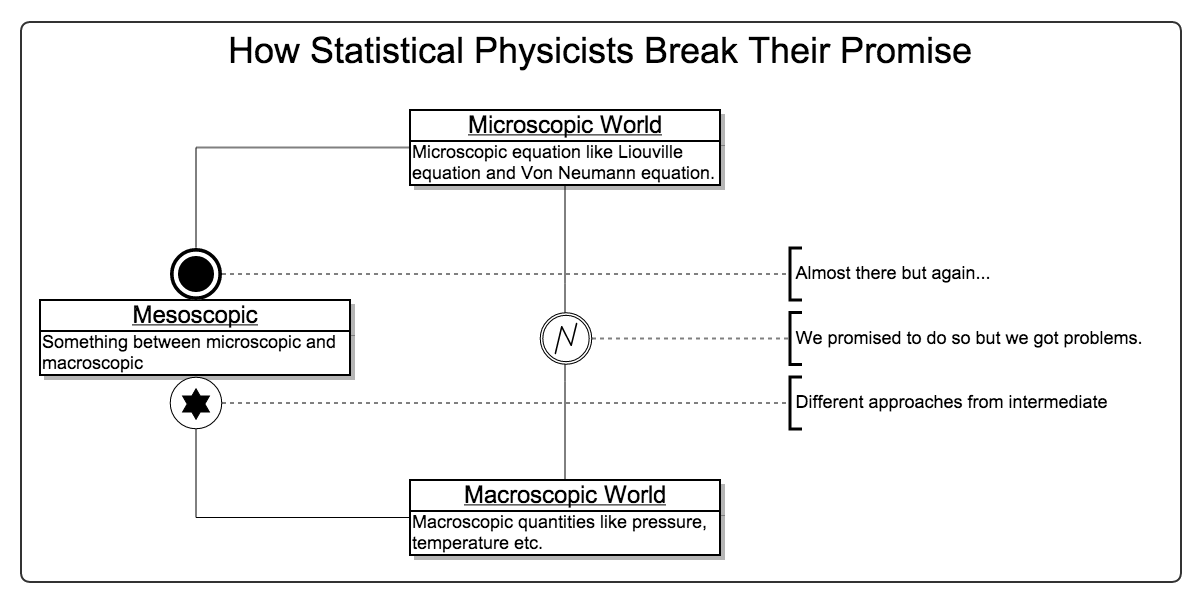
\includegraphics{mesoscopic.png}

We start from microscopic equation, work on them, them trucate at some point, meaning approximation. Then use the approximated result to calculate the marcoscopic quantities.

An example of this method is that we divide a box of gas into two parts. Then we talk about only two states which is LEFT state and RIGHT state instead of the phase space states.

{\hfill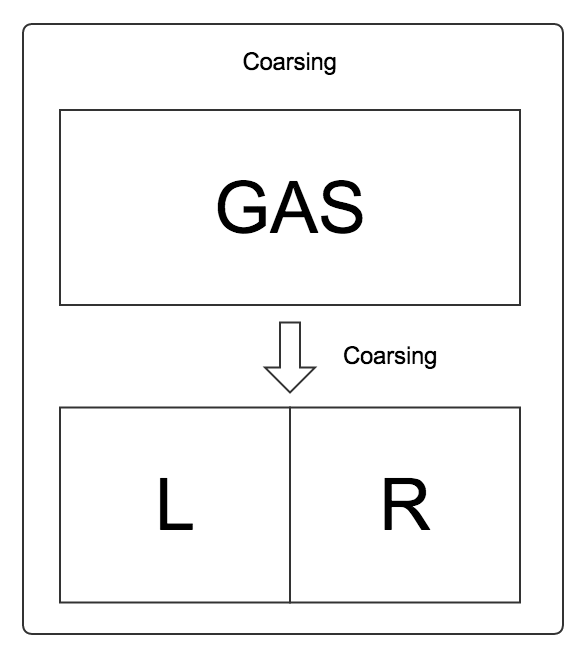
\includegraphics{coarseProcess.png}\hfill}

Now we can write down two equations by intuition,
\begin{gather}
\begin{split}\frac{d P_L}{d t} = T_{LR} P_R - T_{RL}P_L\end{split}\notag\\\begin{split}\end{split}\notag
\end{gather}
and
\begin{gather}
\begin{split}\frac{d P_R}{d t} = T_{RL} P_L - T_{LR}P_R .\end{split}\notag\\\begin{split}\end{split}\notag
\end{gather}
The first equation means that the change of probability that a particle in LEFT state is rate from RIGHT to LEFT time the probability that the particle is in RIGHT state, minus the rate from LEFT state to RIGHT state times the probability that the particle is in LEFT state. This is just simply an linear model of gaining and losing.

It becomes interesting that we can discribe the system in such an easy way. Will it work? We'll see.

More generally, we have
\begin{gather}
\begin{split}\frac{d}{d t} P_\xi = \sum_\mu \left( T_{\xi\mu}P_\mu - T_{\mu\xi} P_{\xi} \right) .\end{split}\notag\\\begin{split}\end{split}\notag
\end{gather}
The important thing is that these equations are linear.

\textbf{Now we can start form these equations instead of the Liouville equation to solve the problem. It's called mesoscopic. The next thing is to connect these mesoscopic equations to the microscopic equations.}


\subsubsection{A Review of Boltzmann Equation \& H Theorem}
\label{nonequilibrium/week8:a-review-of-boltzmann-equation-h-theorem}
The objectives are
\begin{enumerate}
\item {} 
Derive Boltzmann equation from classical scattering theory of rigid balls.

\item {} 
Derive continuity equation from Boltzmann equation.

\item {} 
Prove H theorem.

\item {} 
Understand H theorem.

\end{enumerate}


\paragraph{Boltzmann equation derivation}
\label{nonequilibrium/week8:boltzmann-equation-derivation}
The idea is to find out an equation for one particle probability density $f_j(\vec r, \vec v_j,t)$ by considering the number of particles into this state and out of state due to collision. Since we can find all contributions to $f_j$ by applying scattering theory of classical particles, this equation can be written down explicitly which turns out to be an integrodifferential equation.

The number of particles in a volume $d\vec r d\vec v$ at position $\vec r$ with velocity $\vec v_j$ is
\begin{gather}
\begin{split}f_j(\vec r, \vec v_j,t)d\vec r d\vec v_j .\end{split}\notag\\\begin{split}\end{split}\notag
\end{gather}
Consider the situation after a short time $dt$ we can write down the change of particle numbers due to collision and finally we will get Boltzmann equation.
\begin{gather}
\begin{split}\frac{\partial f_j}{\partial t} + \vec v_j\cdot \nabla _ {\vec r}f_j + \frac{\vec X _ j}{m_j} \cdot \nabla_{\vec v_j} f_j = 2\pi \sum_i \iint \left(f _ i'f _ j' - f _ i f _ j\right) g _ {ij} b \mathrm db  \mathrm d \vec v_i\end{split}\notag\\\begin{split}\end{split}\notag
\end{gather}
where $\vec X$ is the external force on the particle, prime denotes the quantity after collision, $b$ is the impact parameter.

In the derivation, the most important part is to identify the number of particles into and out of this state due to collision.


\paragraph{Boltzmann equation \& Continuity Equation}
\label{nonequilibrium/week8:boltzmann-equation-continuity-equation}
We can derive from Boltzmann equation the Enskog's equation then simplify to continuity equation by picking up an conserved quantity as $\psi_i$ in Enskog's equation.

Continuity equation is alway true for such an conserved system so this results is very conceivable.


\paragraph{H Theorem}
\label{nonequilibrium/week8:h-theorem}
H theorem says that the quantity $H$ can not decrease. The requirements of course should be that in a classical, particle number conserved system.

First define
\begin{gather}
\begin{split}H(t) = \iint  f(\vec r, \vec v, t) \ln  f(\vec r, \vec v, t) d\vec r d\vec v\end{split}\notag\\\begin{split}\end{split}\notag
\end{gather}
Use Boltzmann equation we find out that
\begin{gather}
\begin{split}\frac{d H}{dt} \leq 0\end{split}\notag\\\begin{split}\end{split}\notag
\end{gather}
in which equal sign is valid if\&f
\begin{gather}
\begin{split}f' f_1' = f f_1 .\end{split}\notag\\\begin{split}\end{split}\notag
\end{gather}

\paragraph{H Theorem Discussion}
\label{nonequilibrium/week8:h-theorem-discussion}
There were two objections on H theorem.
\begin{enumerate}
\item {} 
Loschmidt: All collisions can be reversed in the view of classical mechanics;

\item {} 
Zermelo: Poincare recursion theorem says an equilibrium system can go back to inequilibrium.

\end{enumerate}

To Loschmidt's questioning, Boltzmann pointed out that H theorem is a statistical theorem rather than mechanics theorem. Quantities in this theorem like $f$ are statistical average not the quantity of exactly which particle.

Zermelo's objection is not valid because the recursion time is extremely long.


\subsubsection{Footnotes}
\label{nonequilibrium/week8:footnotes}

\subsection{Week 9}
\label{nonequilibrium/week9:week-9}\label{nonequilibrium/week9::doc}
\index{Master Equatioin}

\subsubsection{Master Equation}
\label{nonequilibrium/week9:master-equation}\label{nonequilibrium/week9:index-0}
One way of starting somewhere in between instead of starting from microscopic equations to get macroscopic quantities is coarsing the system and use \textbf{Master Equation}.
\begin{gather}
\begin{split}\frac{dP_\xi}{d t} = \sum_{\mu} \left( T_{\xi\mu} P_\mu - T_{\mu\xi} P_\xi \right)\end{split}\notag\\\begin{split}\end{split}\notag
\end{gather}
which means the rate of $P_\xi(t)$ is determined by the gain and loss of probability.

\begin{notice}{hint}{Hint:}
\textbf{What's the problem of this master equation?}

It's linear. AND it comes from nowhere.
\end{notice}

\index{Chapman-Kolmogorov equation}

\subsubsection{``Derive'' Master Equation}
\label{nonequilibrium/week9:index-1}\label{nonequilibrium/week9:derive-master-equation}
One way of deriving master equation is to start from \DUspan{highlit}{Chapman-Kolmogorov equation} which is
\begin{gather}
\begin{split}P_\xi(t) = \sum_\mu Q_{\xi\mu} P_\mu(t-\tau) .\end{split}\notag\\\begin{split}\end{split}\notag
\end{gather}
This equation describes a discrete and randomwalk process, aka Markov process. In other words, the information about motion is lost with every movement. In this case, all information has been lost before a time interval $\tau$.

The formalism of this equation reminds us the time derivative,
\begin{gather}
\begin{split}\partial_t P_\xi(t) = \lim \frac{P_\xi(t) - P_\xi(t-\tau)}{\tau} .\end{split}\notag\\\begin{split}\end{split}\notag
\end{gather}
To achieve this, notice that
\begin{gather}
\begin{split}\sum_\mu Q_{\mu\xi} = 1.\end{split}\notag\\\begin{split}\end{split}\notag
\end{gather}
\begin{notice}{important}{Important:}
It's very important to see this result clearly. Here we write this identity by regarding that the system must jump out of $\xi$ state because the summation doesn't include the case that $\mu=\xi$.
\end{notice}

Then we can rewrite Chapman-Kolmogorov equation,
\begin{gather}
\begin{split}P_\xi(t) - P_\xi(t-\tau) = \sum_\mu Q_{\xi\mu}P_\mu(t-\tau) - \sum_\mu Q_{\mu\xi} P_\xi(t-\tau) .\end{split}\notag\\\begin{split}\end{split}\notag
\end{gather}
in which we used
\begin{gather}
\begin{split}P_\xi(t-\tau) = \sum_\mu Q_{\mu\xi} P_\xi(t-\tau) .\end{split}\notag\\\begin{split}\end{split}\notag
\end{gather}
Then it seems clear that we can just divide $\tau$ on each side and take the limit that $\tau\rightarrow 0$.
\begin{gather}
\begin{split}\lim_{\tau\rightarrow} \frac{P_\xi(t) - P_\xi(t-\tau)}{\tau} = \lim_{\tau\rightarrow 0} \frac{ \sum_\mu Q_{\xi\mu}P_\mu(t-\tau) - \sum_\mu Q_{\mu\xi} P_\xi(t-\tau) }{\tau}\end{split}\notag\\\begin{split}\end{split}\notag
\end{gather}
Watch out. The right hand side goes to infinity usually. One of the way out is to assume that
\begin{gather}
\begin{split}Q_{ux} = R_{ux}\tau + O(\tau^n)\end{split}\notag\\\begin{split}\end{split}\notag
\end{gather}
with $n > 1$ which introduces a weird property to the system.

\begin{notice}{warning}{Warning:}
By saying a system obeys \DUspan{highlit}{Chapman-Kolmogorov equation} we admit that the system loses information after an time interval $\tau$. Now we take the limit $\tau\rightarrow 0$, which means the system has no memory of the past at all! How to explain this?

Or can we assume that $P(t-\tau)\propto \tau$?
\end{notice}

Anyway, we reach our destination
\begin{gather}
\begin{split}\partial_t P_\xi(t) = \sum_\mu \left( R_{\xi\mu}P_\mu(t) - R_{\mu\xi}P_\xi(t) \right)  .\end{split}\notag\\\begin{split}\end{split}\notag
\end{gather}
\begin{notice}{note}{Note:}
Derivation of master equation can be more rigorous. \footnote{\begin{enumerate}
\setcounter{enumi}{11}
\item {} \begin{enumerate}
\setcounter{enumi}{4}
\item {} 
Reichl. ``A Modern Course in Statistical Physics''.

\end{enumerate}

\end{enumerate}
} This note is a rephrase of Reichl's chapter 6 B. Also refer to Irwin Oppenheim and Kurt E. Shuler's paper. \footnote{
Irwin Oppenheim and Kurt E. Shuler. ``Master Equations and Markov Processes''. \href{http://journals.aps.org/pr/abstract/10.1103/PhysRev.138.B1007}{Phys. Rev. 138, B1007 (1965)} .
}

To do this we need to use conditional probability,
\begin{gather}
\begin{split}P_1(y_1,t_1) P_{1|1}(y_1,t_1|y_2,t_2) = P_2(y_1,t_1;y_2,t_2)\end{split}\notag\\\begin{split}\end{split}\notag
\end{gather}
which means the probability density of variable Y has value $y_1$ at time $t_1$ and $y_2$ at time $t_2$ is given by the probability density of variable Y has value $y_1$ at time $t_1$ times that of it has value $y_1$ at time $t_1$ given it has value $y_2$ at time $t_2$.

Assume that \DUspan{highlit}{the probability density at} $t_n$ \DUspan{highlit}{only depends on that at} $t_{n-1}$, we have
\begin{gather}
\begin{split}P_{n-1|1}(y_1,t_1;\cdots;y_{n-1},t_{n-1}|y_n,t_n) = P_{1|1}(y_{n-1},t_{n-1}|y_n,t_n) = P_{1|1}(y_{n-1},t_{n-1}|y_n,t_n) ,\end{split}\notag\\\begin{split}\end{split}\notag
\end{gather}
if we define the variable in a way that $t_1<t_2< \cdots <t_n$.

\textbf{This assumption means that the system is chaotic enough.} This is called \textbf{Markov process}.

Like the transition coefficients $T_{\xi\mu}$ we defined previously, this $P_{1|1}(y_{n-1},t_{n-1}|y_n,t_n)$ is the \textbf{transition probability}.

To find out the time derivative of $P_1(y_2,t_2)$, we need to write down the time dependence of it,
\begin{gather}
\begin{split}P_(y_1,t_1;y_2,t_2) = P_1(y_1,t_1) P_{1|1}(y_1,t_1|y_2,t_2)\end{split}\notag\\\begin{split}\end{split}\notag
\end{gather}
We integrate over $y_1$,
\begin{gather}
\begin{split}P_1(y_2,t_2) = \int P_1(y_1,t_1)P_{1|1}(y_1,t_1|y_2,t_2)dy_1\end{split}\notag\\\begin{split}\end{split}\notag
\end{gather}
As we can write $t_2=t_1+\tau$,
\begin{gather}
\begin{split}P_1(y_2,t_1+\tau) = \int P_1(y_1,t_1) P _ {1|1}(y_1,t_1|y_2,t_1+\tau) dy_1\end{split}\notag\\\begin{split}\end{split}\notag
\end{gather}
Next we can construct time derivatives of these quantities.
\begin{gather}
\begin{split}\partial_{t_1} P_1(y_2,t_1) = \int \lim_{\tau\rightarrow 0} \frac{\int P_1(y_1,t_1) P _ {1|1}(y_1,t_1|y_2,t_1+\tau) - P_1(y_1,t_1) P _ {1|1}(y_1,t_1|y_2,t_1) }{\tau} dy_1\end{split}\notag\\\begin{split}\end{split}\notag
\end{gather}
The next step is the messy one. Expand the right hand side using Taylor series, which one can find in Reichl's book \footnotemark[1] , we get the expression for this time derivative,
\begin{gather}
\begin{split}\partial_{t} P_1(y_2,t) = \int dy_1 \left( W(y_1,y_2)P_1(y_1,t) - W(y_2,y_1)P_1(y_2,t) \right) .\end{split}\notag\\\begin{split}\end{split}\notag
\end{gather}
This is the \DUspan{highlit}{master equation}.

The reason that $W(y_1,y_2)$ is an transition rate is that it represents ``the probability density perunit time that the system changes from state $y_1$ to $y_2$ in the time interval $t_1\rightarrow t_1 +\tau$ ''. \footnotemark[1]
\end{notice}

\begin{notice}{important}{Important:}
Now we see that \DUspan{highlit}{Markov process} is the hypothesis we need to get master equation? DO NOT mistake this with \DUspan{highlit}{Markov process} ever. There are things unclear in the derivation.

Read Irwin Oppenheim and Kurt E. Shuler's paper for more details. \footnotemark[2]
\end{notice}

\begin{notice}{note}{Note:}
We can find out the \DUspan{highlit}{Chapman-Kolmogorov equation}
\begin{gather}
\begin{split}P_{1|1}(y_1,t_1|y_3,t_3) = \int P _{1|1}(y_1,t_1|y_2,t_2)P_{1|1}(y_2,t_2|y_3,t_3)dy_2\end{split}\notag\\\begin{split}\end{split}\notag
\end{gather}
by comparing the following three equations.
\begin{gather}
\begin{split}P_2(y_1,t_1;y_3,t_3) = \int P_3(y_1,t_1;y_2,t_2;y_3,t_3) dy_2\end{split}\notag\\\begin{split}\end{split}\notag
\end{gather}\begin{gather}
\begin{split}P_3(y_1,t_1;y_2,t_2;y_3,t_3) = P_1(y_1,t_1) P _{1|1}(y_1,t_1|y_2,t_2) P _{1|1}(y_2,t_2|y_3,t_3)\end{split}\notag\\\begin{split}\end{split}\notag
\end{gather}\begin{gather}
\begin{split}\frac{P_2(y_1,t_1;y_3,t_3)}{P_1(y_1,t_1)} = P_{1|1}(y_1,t_1|y_3,t_3)\end{split}\notag\\\begin{split}\end{split}\notag
\end{gather}\end{notice}


\subsubsection{Examples of Master Equation}
\label{nonequilibrium/week9:examples-of-master-equation}
Master equation is
\begin{gather}
\begin{split}\partial_t P_\xi(t) = \sum_\mu \left( R_{\xi\mu}P_\mu(t) - R_{\mu\xi}P_\xi(t) \right) .\end{split}\notag\\\begin{split}\end{split}\notag
\end{gather}

\paragraph{Two States Degenerate System}
\label{nonequilibrium/week9:two-states-degenerate-system}
In such a system master equations are simply
\begin{gather}
\begin{split}\partial_t P_1 = R (P_2 - P_1)\end{split}\notag\\\begin{split}\end{split}\notag
\end{gather}
and
\begin{gather}
\begin{split}\partial_t P_2 = R (P_1 - P_2) .\end{split}\notag\\\begin{split}\end{split}\notag
\end{gather}
To solve the problem, we can choose ``canonical coordinates'',
\begin{gather}
\begin{split}P_+ = P_1+P_2\end{split}\notag\\\begin{split}\end{split}\notag
\end{gather}
and
\begin{gather}
\begin{split}P_- = P_1 - P_2 .\end{split}\notag\\\begin{split}\end{split}\notag
\end{gather}
By adding the master equations, we have
\begin{gather}
\begin{split}\partial_t P_+ = 0\end{split}\notag\\\begin{split}\end{split}\notag
\end{gather}
and
\begin{gather}
\begin{split}\partial_t P_- = -2R P_- .\end{split}\notag\\\begin{split}\end{split}\notag
\end{gather}
Obviously, the solutions to these equations are
\begin{gather}
\begin{split}P_+(t) = P_+(0), \qquad P_-(t) = P_-(0)e^{-2Rt} .\end{split}\notag\\\begin{split}\end{split}\notag
\end{gather}
This result proves that whatever states was the system in initially, it will get to equilibrium finally.

The term $e^{-2R t}$ is a decaying process, or in other words a relaxation process.

\begin{notice}{hint}{Hint:}
In QM, Von Neumann equations is
\begin{gather}
\begin{split}\hat \rho = \hat\rho(0) e^{-i \hat H t/\hbar},\end{split}\notag\\\begin{split}\end{split}\notag
\end{gather}
which is very similar to the solution to the stat mech Liouville equation,
\begin{gather}
\begin{split}P(t) = P(0) e^{-A t},\end{split}\notag\\\begin{split}\end{split}\notag
\end{gather}
where A is a matrix
\begin{gather}
\begin{split}A_{\xi\mu} = -R_{\xi\mu}, \qquad A_{\xi\xi} = \sum_\mu R_{\mu\xi} .\end{split}\notag\\\begin{split}\end{split}\notag
\end{gather}
The difference here is the $i$ in the exponential. Think about decay and rotation.
\end{notice}


\paragraph{Non Degenerate Two State System}
\label{nonequilibrium/week9:non-degenerate-two-state-system}
In such a system, the transfer matrix is
\begin{gather}
\begin{split}A = \begin{pmatrix}A_{11}, A{12} \\ A_{21}, A_{22}\end{pmatrix}\end{split}\notag\\\begin{split}\end{split}\notag
\end{gather}
Then the master equation for this kind of systems is
\begin{gather}
\begin{split}\partial_t \begin{pmatrix}P_1 \\ P_2 \end{pmatrix} = \begin{pmatrix}A_{11}, A_{12}\\ A_{21}, A_{22} \end{pmatrix} \begin{pmatrix}P_1 \\ P_2 \end{pmatrix}\end{split}\notag\\\begin{split}\end{split}\notag
\end{gather}
We will see similar exponential decaying or growing behaviors as degenerate system. The difference is the equilibrium point.
\begin{gather}
\begin{split}\partial_t P_1 = R_{12} P_2 - R_{21} P_1\end{split}\notag\\\begin{split}\end{split}\notag
\end{gather}
shows us that at equilibrium when $\partial_t P_1 = 0$,
\begin{gather}
\begin{split}\frac{R_{12}}{R_{21}} = \frac{P_1(\infty)}{P_2(\infty)}\end{split}\notag\\\begin{split}\end{split}\notag
\end{gather}
which means the coefficients defines the equilibrium point.


\subsubsection{Footnotes}
\label{nonequilibrium/week9:footnotes}

\subsection{Week 10}
\label{nonequilibrium/week10:week-10}\label{nonequilibrium/week10::doc}
\index{Master Equation}

\subsubsection{Solving Master Equations}
\label{nonequilibrium/week10:solving-master-equations}\label{nonequilibrium/week10:index-0}
Master equation, again, is
\begin{gather}
\begin{split}\frac{d P_m}{dt} = \sum_n R_{mn} P_n - \sum_n R_{nm} P_m\end{split}\notag\\\begin{split}\end{split}\notag
\end{gather}
which can be written as a more simple form,
\begin{gather}
\begin{split}\frac{d P_m}{dt} + \sum_n A_{mn}P_n = 0 .\end{split}\notag\\\begin{split}\end{split}\notag
\end{gather}
To figure out the elements of this new matrix $A$, we need to understand how to combine the RHS of master equation.
\begin{gather}
\begin{split}\partial_t \begin{pmatrix} P_1 \\ P_2 \\ \vdots \\ P_N \end{pmatrix} = \begin{pmatrix} 0  & R_{12} & \cdots & R_{1N} \\ R_{21}  & 0 & \cdots & R_{2N} \\ \vdots & \vdots & \ddots & \vdots \\ R_{N1} & R_{N2} & \cdots & 0   \end{pmatrix} \begin{pmatrix} P_1 \\ P_2 \\ \vdots \\ P_N \end{pmatrix}   - \sum_{n}R_{nm} \begin{pmatrix}  1 & 0 & \cdots & 0 \\  0 & 1 & \cdots & 0 \\ \vdots & \vdots & \ddots &  0  \\ 0 & 0 & \cdots & 1  \end{pmatrix}  \begin{pmatrix} P_1 \\ P_2 \\ \vdots \\ P_N \end{pmatrix}\end{split}\notag\\\begin{split}\end{split}\notag
\end{gather}
Since $A_{mm} = \sum_n R_{nm}$ is just a real number, we can combine the two matrices on the RHS, which is
\begin{gather}
\begin{split}\partial_t \begin{pmatrix} P_1 \\ P_2 \\ \vdots \\ P_N \end{pmatrix} + \begin{pmatrix} A_{11}  & -R_{12} & \cdots & -R_{1N} \\ -R_{21}  & A_{22} & \cdots & -R_{2N} \\ \vdots & \vdots & \ddots & \vdots \\ -R_{N1} & -R_{N2} & \cdots & A_{NN}   \end{pmatrix} \begin{pmatrix} P_1 \\ P_2 \\ \vdots \\ P_N \end{pmatrix} = 0  .\end{split}\notag\\\begin{split}\end{split}\notag
\end{gather}
We can define the $\mathbf A$ matrix now.
\begin{gather}
\begin{split}A_{mn} = \begin{cases} -R_{mn} &\quad  n \neq m \\ \sum_{n} R_{nm} & \quad n=m  \end{cases}\end{split}\notag\\\begin{split}\end{split}\notag
\end{gather}
$\mathbf A$ matrix is defined in this way so that we have the master equation becomes
\begin{gather}
\begin{split}\partial_t \mathbf P + \mathbf A \mathbf P = 0 .\end{split}\notag\\\begin{split}\end{split}\notag
\end{gather}
So solve such a matrix equation, we need to diagonalize $\mathbf A$, so that we have a simple solution
\begin{gather}
\begin{split}\mathbf P_{\text{diag}} = e^{- \mathbf A_{\text{diag}} t} .\end{split}\notag\\\begin{split}\end{split}\notag
\end{gather}
The most general way is to diagonalize it using an invertible matrix $\mathbf S$, i.e.,
\begin{gather}
\begin{split}\partial_t \bf S^{-1} P + S^{-1}AS S^{-1} P = 0\end{split}\notag\\\begin{split}\end{split}\notag
\end{gather}
in which we'll define $\mathbf A_{\text{diag}} = \bf S^{-1} P S$ and $\mathbf P_{\text{diag}} = \bf S^{-1} P$. For simplicity, we won't write down the indices from now on.

\begin{notice}{warning}{Warning:}
Is there a mechanism that ensures the $\mathbf A$ is \DUspan{highlit}{invertible} ? If $\mathbf A$ is \DUspan{highlit}{defective} , none of these can be done. Do all physical systems have invertible $\mathbf A$?
\end{notice}

\begin{notice}{hint}{Hint:}
Notice that the form of master equation after this transform is similar to the dynamics of quantum mechanics which is
\begin{gather}
\begin{split}i\hbar \frac{\partial }{\partial t} \ket{\psi} = \hat H \ket{\psi}.\end{split}\notag\\\begin{split}\end{split}\notag
\end{gather}
Another thing is that this form is also similar to Liouville equation,
\begin{gather}
\begin{split}i\partial_t \rho^N = \hat L^N \rho^N .\end{split}\notag\\\begin{split}\end{split}\notag
\end{gather}\end{notice}


\subsubsection{Solving Master Equations: Fourier Transform}
\label{nonequilibrium/week10:solving-master-equations-fourier-transform}
Fourier transform is a quick and efficient way of diagonalizing $\mathbf A$ matrix.

We consider the case that coarsed system has translational symmetry, then we know the value of elements in $\mathbf A$ matrix only dependends on $l:= n-m$. In ohter words,
\begin{gather}
\begin{split}\partial_t P_m  + \sum_n A_{mn} P_n  = 0.\end{split}\notag\\\begin{split}\end{split}\notag
\end{gather}
For translational symmetric system, we can work out discrete Fourier transform to find the normal modes. Define the kth mode as
\begin{gather}
\begin{split}P^k = P_m e^{ikm} .\end{split}\notag\\\begin{split}\end{split}\notag
\end{gather}
Multiply by $e^{ikm}$ on master equstion and sum over m, we get
\begin{gather}
\begin{split}\sum_m \partial_t P_m e^{ikm} + \sum_m \sum_n e^{ikm}A_{m-n} P_n = 0.\end{split}\notag\\\begin{split}\end{split}\notag
\end{gather}
With the definition of kth mode above there, the master equation can be written as
\begin{gather}
\begin{split}\partial_t P^k + \sum_n\sum_m e^{ik(m-n)}A_{m-n} e^{ikn}P_n = 0\end{split}\notag\\\begin{split}\end{split}\notag
\end{gather}
which ``accidently'' diagonalizes the matrix $\mathbf A$. So define the kth mode of $\mathbf A$ as $A^k = \sum_{l=m-n} e^{ik(m-n)}A_{m-n}$ then
\begin{gather}
\begin{split}\partial_t P^k + \sum_{l=m-n}e^{ik(m-n)}A_{m-n} \sum_n e^{ikn}P_n = 0\end{split}\notag\\\begin{split}\end{split}\notag
\end{gather}
is reduced to
\begin{gather}
\begin{split}\partial_t P^k + A^k P^k = 0 \qquad\text{No summation over k!.}\end{split}\notag\\\begin{split}\end{split}\notag
\end{gather}
\begin{notice}{note}{Note:}
Note that summation over n and m is equivalent to summation over n and m-n.
\end{notice}

Finally we have the solution of normal modes,
\begin{gather}
\begin{split}P^k(t) = P^k(0) e^{-A^k t} .\end{split}\notag\\\begin{split}\end{split}\notag
\end{gather}
To find out the final solution, inverse Fourier transform on kth mode,
\begin{gather}
\begin{split}P_m(t) = \frac{1}{N} \sum_k P^k(t) e^{-ikm} .\end{split}\notag\\\begin{split}\end{split}\notag
\end{gather}
\begin{notice}{important}{Important:}
Note that due to the Born van Karman BC we chose,
\begin{gather}
\begin{split}e^{ikm} = e^{ik(m+N)}\end{split}\notag\\\begin{split}\end{split}\notag
\end{gather}
which leads to
\begin{gather}
\begin{split}k=\frac{2\pi}{N} .\end{split}\notag\\\begin{split}\end{split}\notag
\end{gather}
Discrete transform will become integral if we are dealing with continous systems, which will be achieved by using the following transformation,
\begin{gather}
\begin{split}\frac{1}{N}\sum_k  \rightarrow \frac{1}{2\pi} \int dk\end{split}\notag\\\begin{split}\end{split}\notag
\end{gather}
We write down this identity like transformation because the discrete result has the form $\frac{1}{N}\sum_k$.
\end{notice}


\subsubsection{Finite Chain with Nearest Neighbor Interactions}
\label{nonequilibrium/week10:finite-chain-with-nearest-neighbor-interactions}
In this simple case, the transfer is
\begin{gather}
\begin{split}R_{mn} = F(\delta_{m,n-1}+ \delta_{m,n+1}) .\end{split}\notag\\\begin{split}\end{split}\notag
\end{gather}
So master equation becomes
\begin{gather}
\begin{split}\partial_t P_m = F(P_{n+1} + P_{n-1}) -2F P_m .\end{split}\notag\\\begin{split}\end{split}\notag
\end{gather}
\begin{notice}{note}{Note:}
There is no need to use the definition of $\mathbf A$ matrix in this simple case.
\end{notice}

Discrete Fourier transform,
\begin{gather}
\begin{split}\partial_t P^k  = F(e^{ikm} P_{m+1} + e^{ikm} P_{m-1} -2 P^k) .\end{split}\notag\\\begin{split}\end{split}\notag
\end{gather}
Combine terms,
\begin{gather}
\begin{split}\partial_t P^k = 4F\sin^2\frac{k}{2} .\end{split}\notag\\\begin{split}\end{split}\notag
\end{gather}
The solution for kth mode should be
\begin{gather}
\begin{split}P^k(t) = P^k(0) e^{-4F \sin^2\frac{k}{2} t} .\end{split}\notag\\\begin{split}\end{split}\notag
\end{gather}
Inverse Fourier transform gives us the result of
\begin{gather}
\begin{split}P_m(t)  = \frac{1}{N} \sum_ {k} P^k(t) e^{-i km} .\end{split}\notag\\\begin{split}\end{split}\notag
\end{gather}
The last thing is to find out the value of $k$. Apply Born-Von Karman boundary condition, we find that $k$ is quantized,
\begin{gather}
\begin{split}k = \frac{2\pi}{N} n, \qquad n=0,1,2, \cdots, N-1 .\end{split}\notag\\\begin{split}\end{split}\notag
\end{gather}

\paragraph{Matrix Form}
\label{nonequilibrium/week10:matrix-form}
To make it clear, we'll redo this problem in matrix form.

First of all, write down master equation for this problem again,
\begin{gather}
\begin{split}\partial_t P_m = F(P_{n+1} + P_{n-1}) -2F P_m .\end{split}\notag\\\begin{split}\end{split}\notag
\end{gather}
In the form of matrix, we have
\begin{gather}
\begin{split}\partial_t \begin{pmatrix} P_1 \\ P_2 \\ P_3 \\ P_4 \\ P_5 \\ P_6 \end{pmatrix} + F \begin{pmatrix}  2 & -1 & 0 & 0 & 0 & -1 \\ -1 & 2 & -1 & 0 & 0 & 0 \\0 & -1 & 2 & -1 & 0 & 0 \\ 0 & 0 & -1 & 2 & -1 & 0 \\ 0 & 0 & 0 & -1 & 2 & -1 \\ -1 & 0 & 0 & 0 & -1 & 2 \end{pmatrix} \begin{pmatrix} P_1 \\ P_2 \\ P_3 \\ P_4 \\ P_5 \\ P_6 \end{pmatrix} = 0\end{split}\notag\\\begin{split}\end{split}\notag
\end{gather}
\begin{notice}{hint}{Hint:}
An easy way to get the matrix is to write down the $\mathbf R$ matrix which has 0 diagonal elements, construct $\mathbf A$ matrix by adding minus sign to all elements and put the sum of the original elements at the diagonal in the corresponding line. Pay attention to the signs.

Another propertity worth talking about is the \DUspan{highlit}{additive of the matrices}. \DUspan{highlit}{A more complicated system can be decomposed into several simple systems.}
\end{notice}

The technique used to solve this problem is to diagonalize the 6 times 6 matrix because we can then just write down the solutions.

The way to do this is exactly what have did in the previous part, that is defining new quantities. Then we have in matrix form
\begin{gather}
\begin{split}\partial_t \begin{pmatrix} P^{k_1} \\ P^{k_2}\\ P^{k_3}\\ P^{k_4}\\ P^{k_5}\\ P^{k_6} \end{pmatrix} + 4F \begin{pmatrix} \sin^2\frac{k_1}{2} 0 & 0 & 0 & 0 & 0 \\ 0 &  \sin^2\frac{k_2}{2} & 0 & 0 & 0 & 0 \\ 0 & 0 &  \sin^2\frac{k_3}{2} & 0 & 0 & 0 \\ 0 & 0 & 0 & \sin^2\frac{k_4}{2} & 0 & 0 \\ 0 & 0 & 0 & 0 &  \sin^2\frac{k_5}{2} & 0 \\ 0 & 0 & 0 & 0 & 0 &  \sin^2\frac{k_6}{2}   \end{pmatrix} \begin{pmatrix} P^{k_1} \\ P^{k_2}\\ P^{k_3}\\ P^{k_4}\\ P^{k_5}\\ P^{k_6} \end{pmatrix} = 0\end{split}\notag\\\begin{split}\end{split}\notag
\end{gather}
By writing in this form, we imediately know why diagonalizing is the thing we eager to do. The solutions are just
\begin{gather}
\begin{split}P^k(t) = P^k(0) e^{-4F\sin^2(k/2) t} .\end{split}\notag\\\begin{split}\end{split}\notag
\end{gather}
\begin{notice}{hint}{Hint:}
Recall that the elements in the diagonailized $\mathbf A_{\text{diag}}$ matrix are just the eigenvalues of $\mathbf A$ matrix with corresponding eigenvectors. So in other words, the way to solve this kind of descrete master equations is to solve the eigen problem of $\mathbf A$ matrix and then find the eigen modes and finally inverse transform back to $P_m(t)$.
\end{notice}


\subsubsection{Infinite Chain with Nearest Neighbor Interactions}
\label{nonequilibrium/week10:infinite-chain-with-nearest-neighbor-interactions}
We have exactly the same equations as in finite chain. The difference lies in the boundary condition where $N\rightarrow \infty$ and
\begin{gather}
\begin{split}\frac{1}{N}\sum_k \rightarrow \frac{1}{2\pi}\int dk .\end{split}\notag\\\begin{split}\end{split}\notag
\end{gather}
\begin{notice}{hint}{Hint:}
The way to check this result is to check the sum of unit probability.
\begin{gather}
\begin{split}\frac{1}{N}\sum_{k=1}^{N} 1 = 1 \Leftrightarrow \frac{1}{2\pi}\int_{-\pi}^{\pi} 1 dk = 1\end{split}\notag\\\begin{split}\end{split}\notag
\end{gather}\end{notice}

So the solutions are
\begin{gather}
\begin{split}P_m(t) &= \frac{1}{2\pi} \int _{-\pi}^{\pi} P^k(0) e^{-2F(1-\cos{k})t} e^{-ikm} dk \\ &=  P^k(0)  e^{-2Ft} \frac{1}{2\pi} \int_{-\pi}^{\pi} e^{2Ft\cos{k}} e^{-ikm} dk \\
& = P^k(0)  e^{-2Ft} \mathrm{I_m}(2Ft)\end{split}\notag\\\begin{split}\end{split}\notag
\end{gather}
\index{Modified Bessel Function}
\begin{notice}{important}{Important:}
\textbf{Vocabulary}: \DUspan{highlit}{Modified Bessel function} is defined as
\begin{gather}
\begin{split}\mathrm{I_m} (z) = \frac{1}{2\pi}\int_{-\pi}^{\pi} e^{-ikm} e^{z\cos{k}} dk  .\end{split}\notag\\\begin{split}\end{split}\notag
\end{gather}
Since the argument has imaginary part, this is also called Bessel function of imaginary argument.

Check out more properties about this function in vocabulary part.
\begin{figure}[htbp]
\centering
\capstart

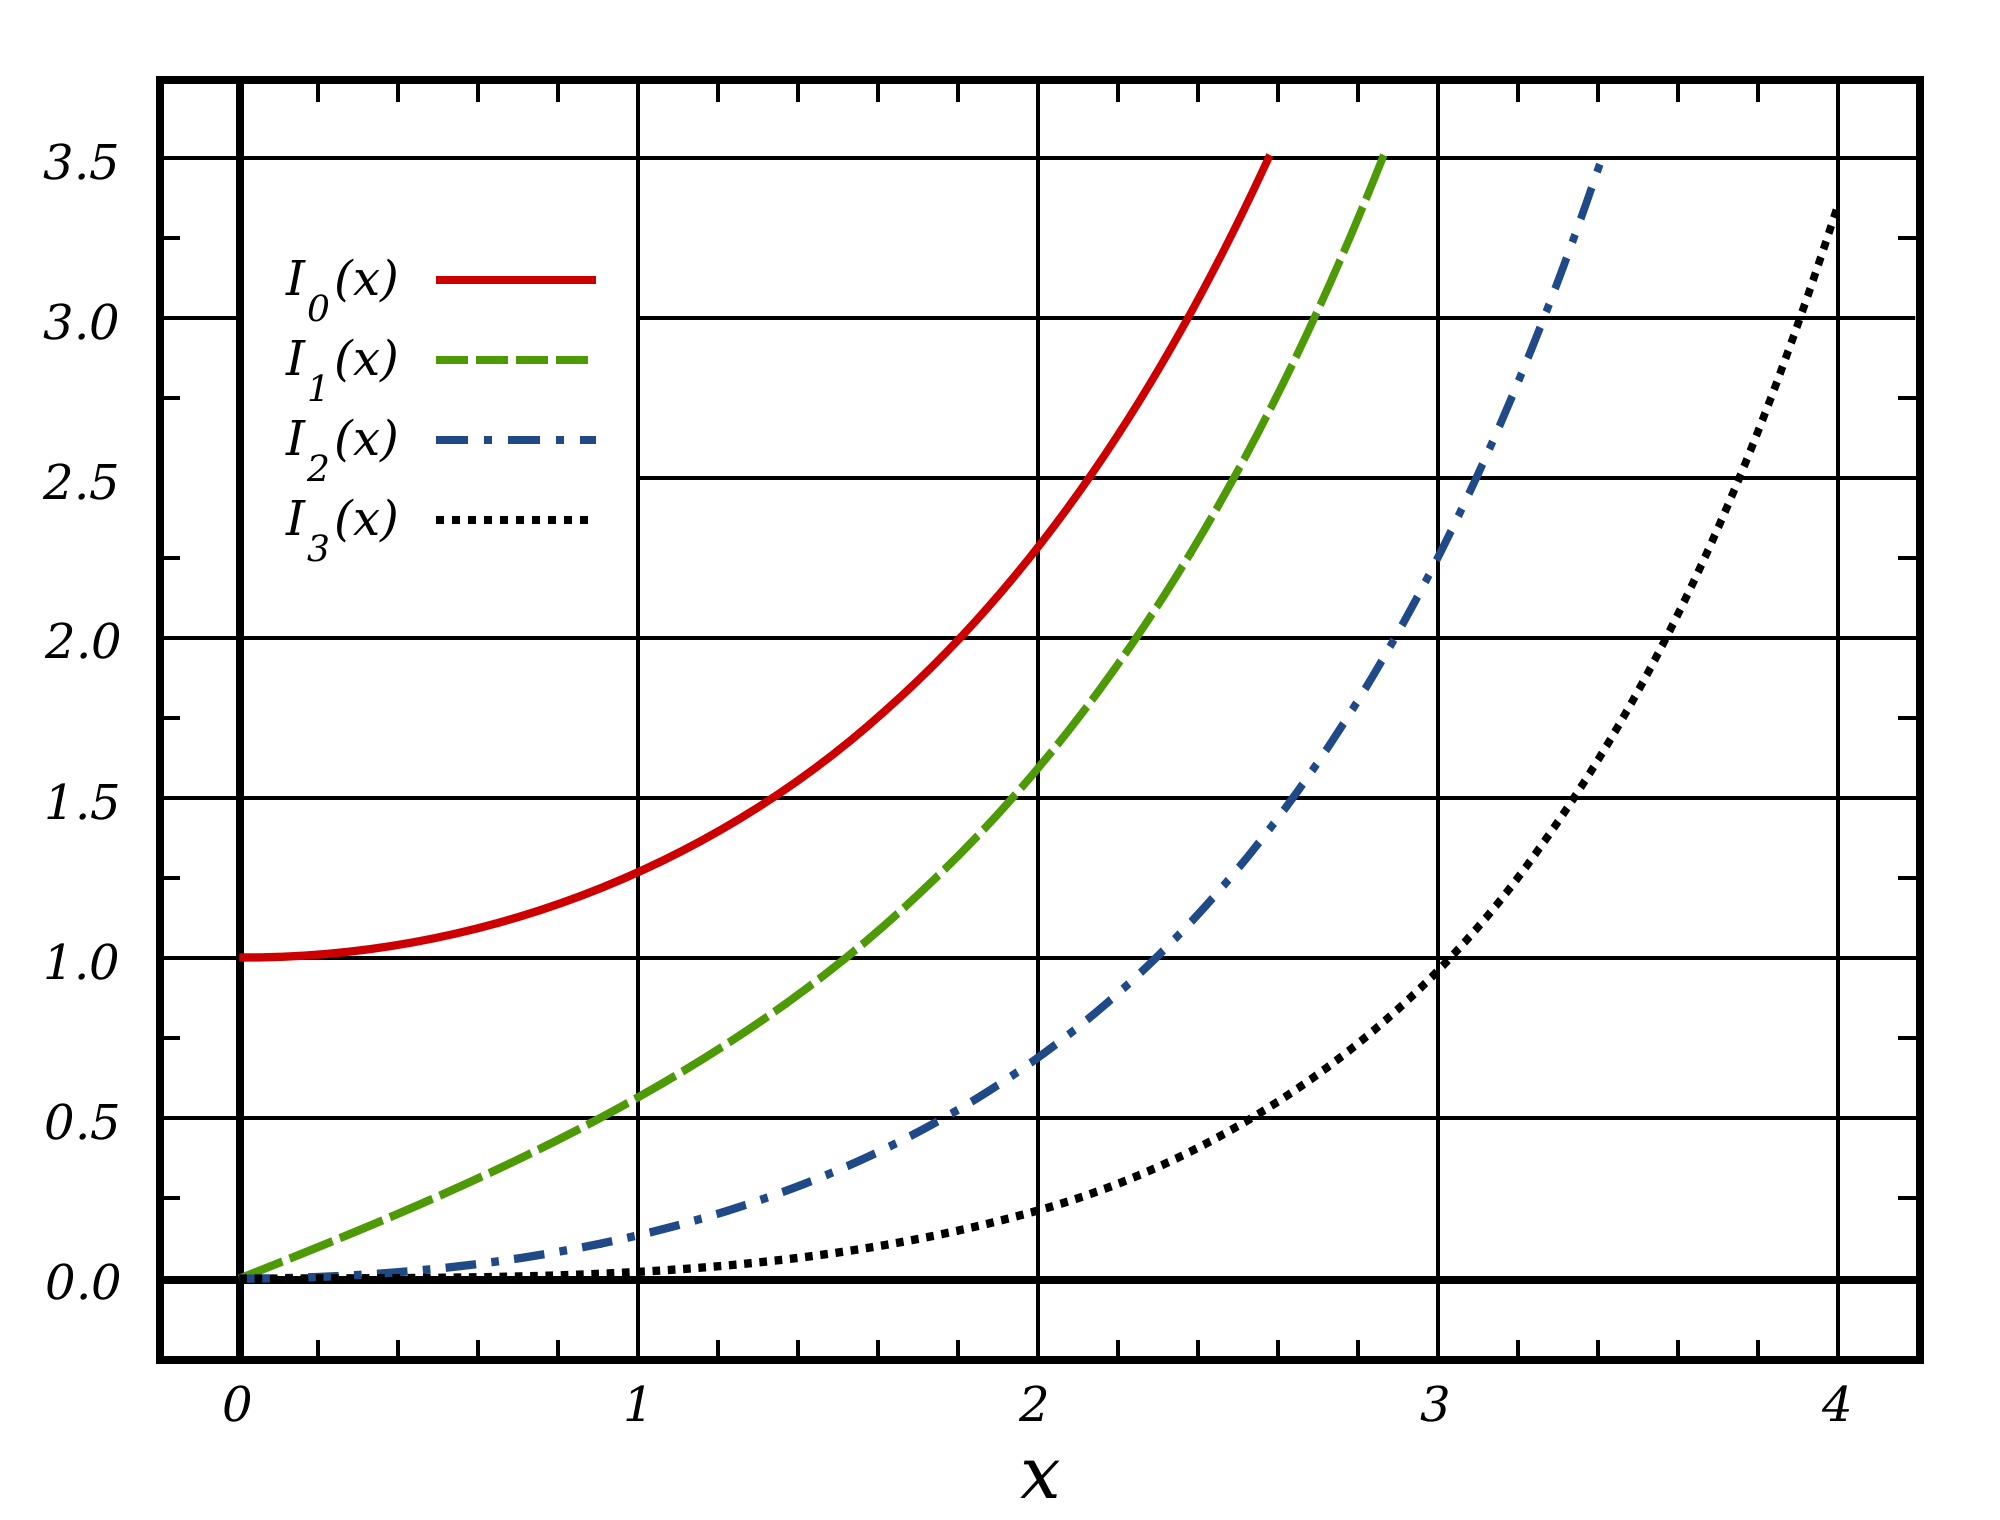
\includegraphics[width=1.000\linewidth]{besselIFunctions1stKind.png}
\caption{\href{https://en.wikipedia.org/wiki/File:BesselI\_Functions\_(1st\_Kind,\_n\%3D0,1,2,3).svg}{https://en.wikipedia.org/wiki/File:BesselI\_Functions\_(1st\_Kind,\_n\%3D0,1,2,3).svg}}\end{figure}
\end{notice}


\subsubsection{2D Lattice}
\label{nonequilibrium/week10:d-lattice}
A 2D lattice image is shown below \href{https://commons.wikimedia.org/wiki/File:Equilateral\_Triangle\_Lattice.svg}{with image cridet of Jim Belk (public domain)}.
\begin{figure}[htbp]
\centering
\capstart

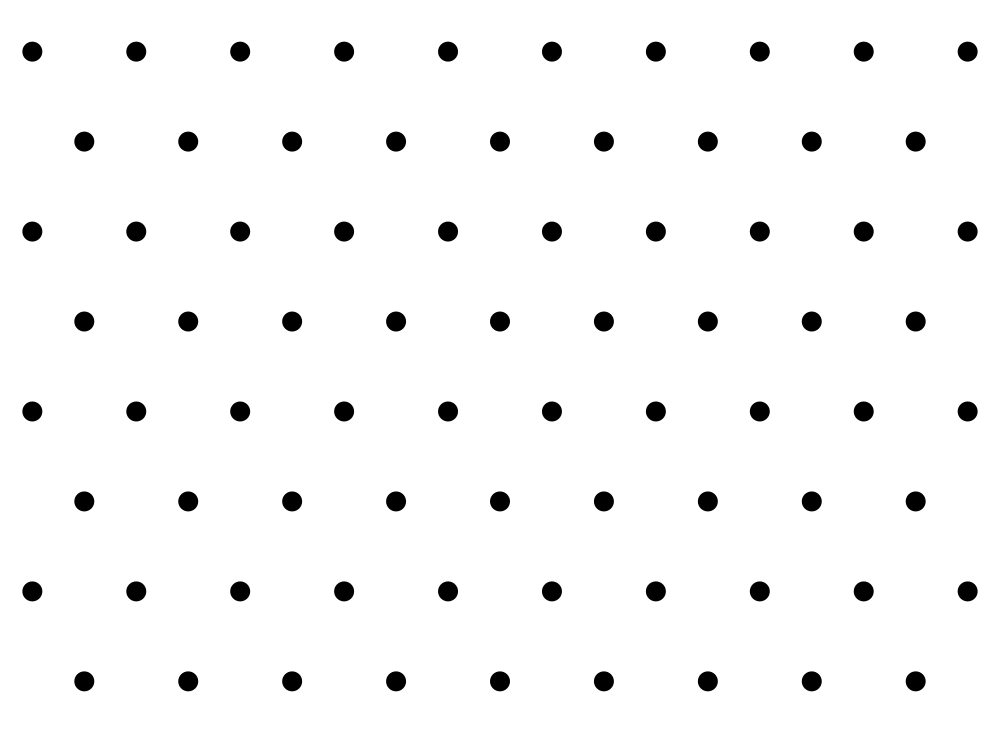
\includegraphics{equilateralTriangleLattice.png}
\caption{An equilateral triangle lattice}\end{figure}

Note that we have translational symmetry in both x and y direction. So the solution is simply the product of solutions to two directioins,
\begin{gather}
\begin{split}P_m(t) = e^{-2(F_x+F_y)t} \mathrm{I_m}(2F_xt) \mathrm{I_m}(2F_y t)\end{split}\notag\\\begin{split}\end{split}\notag
\end{gather}

\subsubsection{Continuum Limit}
\label{nonequilibrium/week10:continuum-limit}
Suppose we have a continuum system,
\begin{gather}
\begin{split}\partial_t P_m &= F(P_{m-1} + P_{m+1}) - 2FP_m \\
& = F(P_{m+1}-P_m -(P_m-P_{m-1})) \\
& = F \epsilon^2 \frac{ (P_{m+1}-P_m)/\epsilon -(P_m-P_{m-1})/\epsilon )  }{\epsilon}\end{split}\notag\\\begin{split}\end{split}\notag
\end{gather}
We can identify the form of derivatives but RHS becomes zero if $F$ is a constant when we take the limit $\epsilon \rightarrow 0$.

It does make sense that $F$ actually increases when the distance between two sites becomes smaller. And the way to reconcile the zero problem is to assume that
\begin{gather}
\begin{split}F = \frac{D}{\epsilon^2} .\end{split}\notag\\\begin{split}\end{split}\notag
\end{gather}
Then we have the diffusion equation.
\begin{gather}
\begin{split}\frac{\partial P(x,t)}{\partial t} = D\frac{\partial^2 P(x,t)}{\partial x^2}\end{split}\notag\\\begin{split}\end{split}\notag
\end{gather}
.


\subsection{Week 11}
\label{nonequilibrium/week11:week-11}\label{nonequilibrium/week11::doc}
\index{Irrersibility}

\subsubsection{Irrersibility}
\label{nonequilibrium/week11:irrersibility}\label{nonequilibrium/week11:index-0}
Fourier series are complete,
\begin{gather}
\begin{split}F(x) = \sum_{n=0}^{n=\infty} a_n \cos(\omega_n t) .\end{split}\notag\\\begin{split}\end{split}\notag
\end{gather}
Any equations can be expanded using Fourier series including the decay behavior we have seen in previous lectures.

However the problem is, for finite system, the expansion is not really complete. The series composed by all these finite components might not be decay and recurrence could happen. But the time needed for recurrence is so long that we never see it.


\subsubsection{Master Equation}
\label{nonequilibrium/week11:master-equation}
Solution to descrete master equation with nearest neighbour interaction is
\begin{gather}
\begin{split}P_m(t) = P_m(0)I_m(2Ft)e^{-2Ft}\end{split}\notag\\\begin{split}\end{split}\notag
\end{gather}
where $I_m(2Ft)e^{-2Ft}$ is the \DUspan{highlit}{propagator}.

Sometimes we want to know where the particle goes after a while. In this case, we should find out \DUspan{highlit}{second moment}, $\langle m^2 \rangle$.

To find out second moment, take the second derivative of $P^k(t)$,
\begin{gather}
\begin{split}P^k &=\sum_m P_m e^{imk} \\
\frac{\partial^2}{\partial k^2} P^k &= \sum_m P_m (i m)^2 e^{imk} .\end{split}\notag\\\begin{split}\end{split}\notag
\end{gather}
Set $k=0$, we have
\begin{gather}
\begin{split}\langle m^2 \rangle := \sum_m m^2 P_m =\frac{\partial^2}{\partial k^2} .\end{split}\notag\\\begin{split}\end{split}\notag
\end{gather}
\begin{notice}{note}{Note:}
So we don't need to calculate $P_m(t)$ which takes a lot of time to calculate.
\end{notice}

\begin{notice}{hint}{Hint:}
No mater what kind of interaction the system has,
\begin{gather}
\begin{split}P^k(t) = P^k(0) e^{-\cdots}\end{split}\notag\\\begin{split}\end{split}\notag
\end{gather}
is alway true.
\end{notice}


\subsubsection{Continuum Limit}
\label{nonequilibrium/week11:continuum-limit}
In continuum limit, our master equation becomes
\begin{gather}
\begin{split}\frac{\partial}{\partial t} P = D \frac{\partial^2 P}{\partial x^2}\end{split}\notag\\\begin{split}\end{split}\notag
\end{gather}
which is infact a diffusion equation.

\begin{notice}{hint}{Hint:}\begin{itemize}
\item {} 
Propagators of this equation is gaussian like.

\item {} 
Propagators of discrete master equation is a decay, $I_m(2Ft)e^{-2Ft}$.

\end{itemize}
\end{notice}

\begin{notice}{warning}{Warning:}
In principle, we can take some limit of the master equation propagator and make it the diffusion propagator.
\end{notice}

Second moment of diffusion equaiton is the Einstein brownian motion result
\begin{gather}
\begin{split}\langle x^2 \rangle = 2 D t .\end{split}\notag\\\begin{split}\end{split}\notag
\end{gather}
where
\begin{gather}
\begin{split}\langle x^2\rangle &:= \int_{-\infty}^{+\infty} P(x,t) x^2 dx \\
\langle m^2 \rangle &:= \sum_{-\infty}^{+\infty} P_m(t) m^2  .\end{split}\notag\\\begin{split}\end{split}\notag
\end{gather}

\subsubsection{Landau-Teller Master Equation}
\label{nonequilibrium/week11:landau-teller-master-equation}
Consider a system in a heat bath, we can expand the system to second order and the system becomes a HO or HOs. Fermi golden rule tells us that HO can only have nearest energy transition.


\paragraph{Continuous Grid or Energy}
\label{nonequilibrium/week11:continuous-grid-or-energy}
\begin{notice}{note}{Note:}
Different energy states in a system should have
\begin{gather}
\begin{split}\frac{f_1}{f_1'} = e^{-\frac{\epsilon_1 - \epsilon_1'}{kT}} .\end{split}\notag\\\begin{split}\end{split}\notag
\end{gather}
And $f_1\neq f_1'$ most of the time. For the case of HO
\begin{gather}
\begin{split}\frac{f_1}{f_1'} = e^{-\frac{\hbar \omega}{kT}} .\end{split}\notag\\\begin{split}\end{split}\notag
\end{gather}\end{notice}

Here in such a system
\begin{gather}
\begin{split}\frac{d}{dt}P_m =& k \left[(m+1)(P_{m+1} - e^{-\beta \hbar \omega} P_m)\right. \\
& \left. +m(e^{-\beta \hbar\omega} P_{m-1} - P_m)  \right] .\end{split}\notag\\\begin{split}\end{split}\notag
\end{gather}
\begin{notice}{note}{Note:}
Transition
\begin{gather}
\begin{split}\frac{d}{dt}P_m =& (R_{m,m+1}P_{m+1} -  R_{m,m-1}P_{m-1}) \\
& - (R_{m+1,m}P_m + R_{m-1,m}P_m)\end{split}\notag\\\begin{split}\end{split}\notag
\end{gather}
is called \DUspan{highlit}{Landau-Teller master equation}. It's good for non-translational-invariant system.
\end{notice}


\subsubsection{1-D Discrete Master Equation}
\label{nonequilibrium/week11:d-discrete-master-equation}\begin{gather}
\begin{split}\frac{d}{dt}P_m= F(P_{m+1} + P_{m-1} -2 P_m)\end{split}\notag\\\begin{split}\end{split}\notag
\end{gather}
with solution
\begin{gather}
\begin{split}P_m(t) = \sum_n \Pi_{m-n}(t) P_n(0)\end{split}\notag\\\begin{split}\end{split}\notag
\end{gather}
in which $\Pi_{m-n}(t) = e^{-2Ft}I_m(2Ft)$ is the propagator.

\begin{notice}{hint}{Hint:}
If the sytem has no translational invariance,
\begin{gather}
\begin{split}P_m(t) = \sum_n \Pi_{m,n}(t) P_m(0)\end{split}\notag\\\begin{split}\end{split}\notag
\end{gather}
propagator becomes $\Pi_{m,n}(t)$ depends on both m and n.
\end{notice}


\subsubsection{Continuum Limit}
\label{nonequilibrium/week11:id1}\begin{gather}
\begin{split}\frac{\partial}{\partial t}P(x,t) = D\frac{\partial^2}{\partial x^2} P(x,t)\end{split}\notag\\\begin{split}\end{split}\notag
\end{gather}\begin{gather}
\begin{split}\Pi(x,t) = \cdots e^{-\frac{x^2}{\cdots}}/\sqrt{\cdots t}\end{split}\notag\\\begin{split}\end{split}\notag
\end{gather}
Fourier transform
\begin{gather}
\begin{split}\frac{\partial P_F(k,t)}{\partial t} = - D k^2 P_F(k,t)\end{split}\notag\\\begin{split}\end{split}\notag
\end{gather}
Solution
\begin{gather}
\begin{split}P_F(k,t) = P_F(k,0) e^{-Dk^2t}\end{split}\notag\\\begin{split}\end{split}\notag
\end{gather}
Inverse
\begin{gather}
\begin{split}P(x,t) = \int \Pi(x-x',t) P(x',0) dx'\end{split}\notag\\\begin{split}\end{split}\notag
\end{gather}

\subsection{Week 12}
\label{nonequilibrium/week12:week-12}\label{nonequilibrium/week12::doc}
\index{Propagator}

\subsubsection{Propagator}
\label{nonequilibrium/week12:index-0}\label{nonequilibrium/week12:propagator}
To solve master equation, we usually find out the propagator $\Pi(x-x',t)$. For simple discrete master equation, we have the propagator with the form $I_m(2Ft)e^{-2Ft}$.
\begin{figure}[htbp]
\centering
\capstart

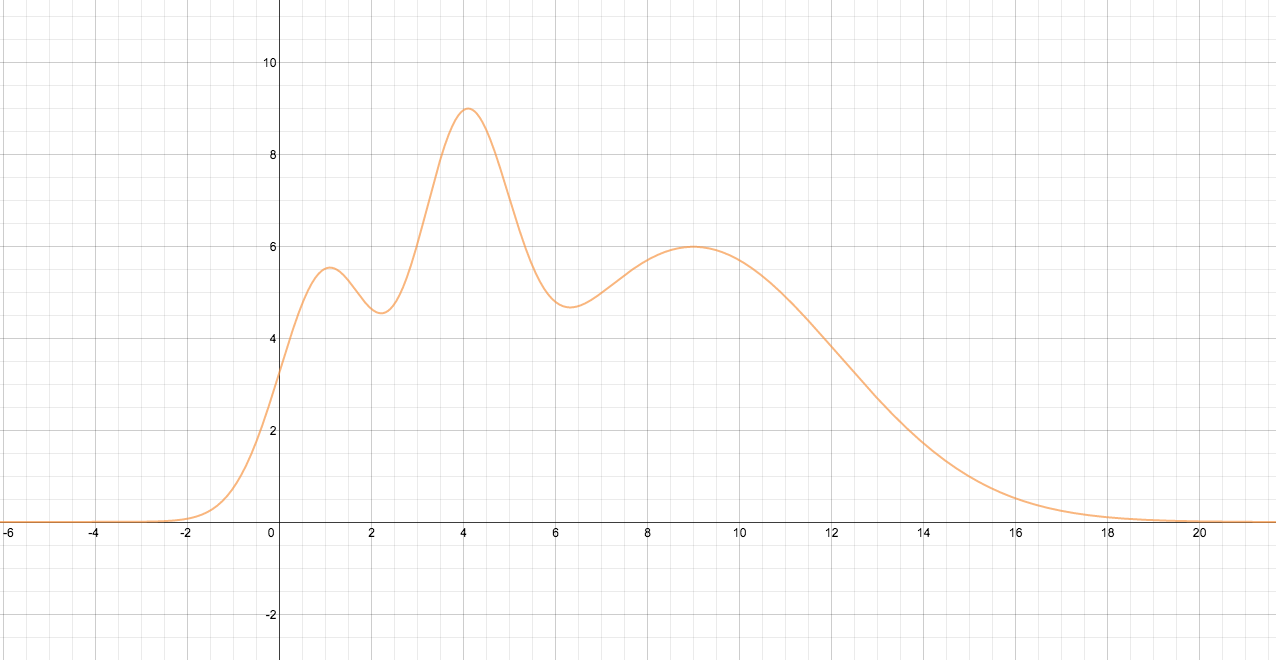
\includegraphics[width=0.900\linewidth]{distInit.png}
\caption{Some initial distribution}\end{figure}

For continuous master equation which is the diffusion equation, given the initial distribution, it evolves according to
\begin{gather}
\begin{split}\frac{\partial}{\partial t} P(x,t) = \zeta \frac{\partial}{\partial x} P(x,t) + D \frac{\partial^2}{\partial x^2} P(x,t) .\end{split}\notag\\\begin{split}\end{split}\notag
\end{gather}
Then after infinite time, we have the final distribution.
\begin{figure}[htbp]
\centering
\capstart

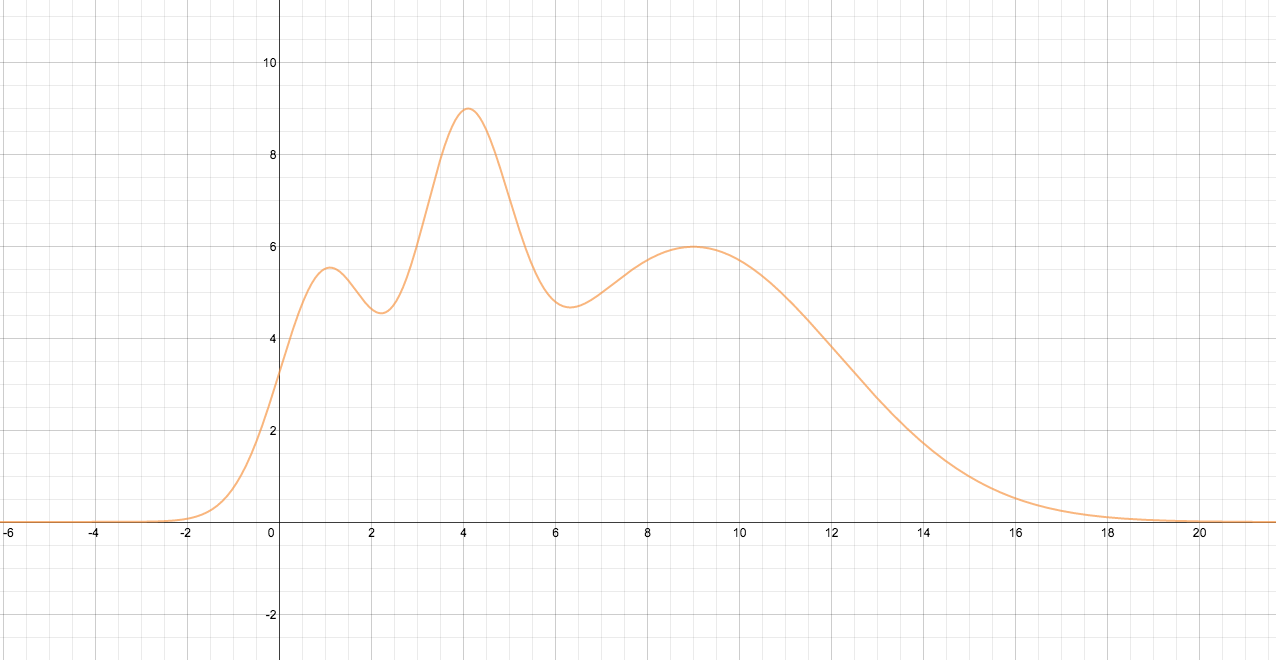
\includegraphics[width=0.900\linewidth]{distInit.png}
\caption{Some final distribution}\end{figure}

\textbf{As long as the system has translational or rotational invariance, we can use Fourier transform to reduce the higher order derivatives to solve the equation.}

For $\zeta =0$, there is only diffusion, so we have translational invariance. Fourier transform for continuous equation is
\begin{gather}
\begin{split}\frac{\partial}{\partial x} e^{ikx}=ike^{ikx} &\implies \frac{\partial}{\partial x} \to ik \\
\frac{\partial^2}{\partial x^2} e^{ikx} = -k^2 e^{ikx} & \implies \frac{\partial^2}{\partial x^2} \to -k^2\end{split}\notag\\\begin{split}\end{split}\notag
\end{gather}
So we can write down the transformed equation right away (for $\zeta=0$ case).
\begin{gather}
\begin{split}\frac{\partial}{\partial t}P^k = -D k^2 P^k\end{split}\notag\\\begin{split}\end{split}\notag
\end{gather}
and the solution to this equation is
\begin{gather}
\begin{split}P^k(t) = P^k(0) e^{-D k^2 t} .\end{split}\notag\\\begin{split}\end{split}\notag
\end{gather}
To find out the propagator, we complete the square,
\begin{gather}
\begin{split}P(x,t) & = \int P(k,0) e^{-Dk^2t+ikx} dk \\
& = \int P(k,0) e^{-\frac{x^2}{4Dt}} e^{-Dt(k-\frac{ix}{2Dt})^2 }dk \\
& = e^{-\frac{x^2}{4Dt}}  \int P(k,0) e^{-Dt(k-\frac{ix}{2Dt})^2 }dk\end{split}\notag\\\begin{split}\end{split}\notag
\end{gather}
The propagator is finally
\begin{gather}
\begin{split}\Pi(x,t) = \frac{e^{-\frac{x^2}{4Dt}}}{\sqrt{4\pi Dt}}\end{split}\notag\\\begin{split}\end{split}\notag
\end{gather}
\begin{notice}{warning}{Warning:}
Somehow I can't derive it. Stupid.
\end{notice}

\begin{notice}{hint}{Hint:}
There might be sigularity in the propagator. One example of it is logorithm sigularity in 2D.
\end{notice}


\subsubsection{Bias in Master Equation}
\label{nonequilibrium/week12:bias-in-master-equation}
When $\zeta\neq 0$, the first term on RHS is a decay or viscous term.
\begin{gather}
\begin{split}\frac{\partial}{\partial t}P(x,t) = \zeta \frac{\partial}{\partial x}P(x,t) + D\frac{\partial^2}{\partial x^2}P(x,t)\end{split}\notag\\\begin{split}\end{split}\notag
\end{gather}
\begin{notice}{hint}{Hint:}
To check the properties of $\zeta$, set $D=0$.
\begin{gather}
\begin{split}\frac{\partial}{\partial t} P = \zeta \frac{\partial}{\partial x} P \Rightarrow P\propto e^{k_w(\omega + \zeta t)}\end{split}\notag\\\begin{split}\end{split}\notag
\end{gather}
So we know that when $k_w > 0$,
\begin{enumerate}
\item {} 
$\zeta > 0$ : exponential grow;

\item {} 
$\zeta < 0$ : decay

\end{enumerate}
\end{notice}

We can Fourier transform then complete the square to solve this kind of problem.

\begin{notice}{hint}{Hint:}
This formalism is very much like the \DUspan{highlit}{Gauge Transformation}. We define a new derivative
\begin{gather}
\begin{split}\frac{\partial}{\partial x} \to \frac{\partial}{\partial x} + \Gamma(x)\end{split}\notag\\\begin{split}\end{split}\notag
\end{gather}
Then we put this new derivative into diffusion equation,
\begin{gather}
\begin{split}& \frac{\partial}{\partial t} P(x,t) = D\frac{\partial^2}{\partial x^2} P(x,t) \\
\to & \frac{\partial}{\partial t} P(x,t) = D \left(\frac{\partial^2}{\partial x^2} P(x,t) + 2\Gamma\frac{\partial}{\partial x}P(x,t) \right) + D\left( P\left( 2\Gamma^2 + \frac{\partial}{\partial x} \Gamma \right) \right)\end{split}\notag\\\begin{split}\end{split}\notag
\end{gather}
Now we define $\zeta := 2\Gamma$, and let $2\Gamma^2 + \frac{\partial}{\partial x} \Gamma$. \footnote{
This is \DUspan{highlit}{Riccati's equation}. More information \href{http://www.wolframalpha.com/input/?i=solve\%5Bdf\%2Fdx\%3D\%3D-2f\%5E2\%5D}{here}.
}  The diffusion equation under this kind of transformation becomes the one we need.

\DUspan{highlit}{Does it imply that the diffusion equation and gauge transformation are related?}

We might find some symmetry using this method.
\end{notice}


\subsubsection{Smoluchowski Equation}
\label{nonequilibrium/week12:smoluchowski-equation}\begin{figure}[htbp]
\centering
\capstart

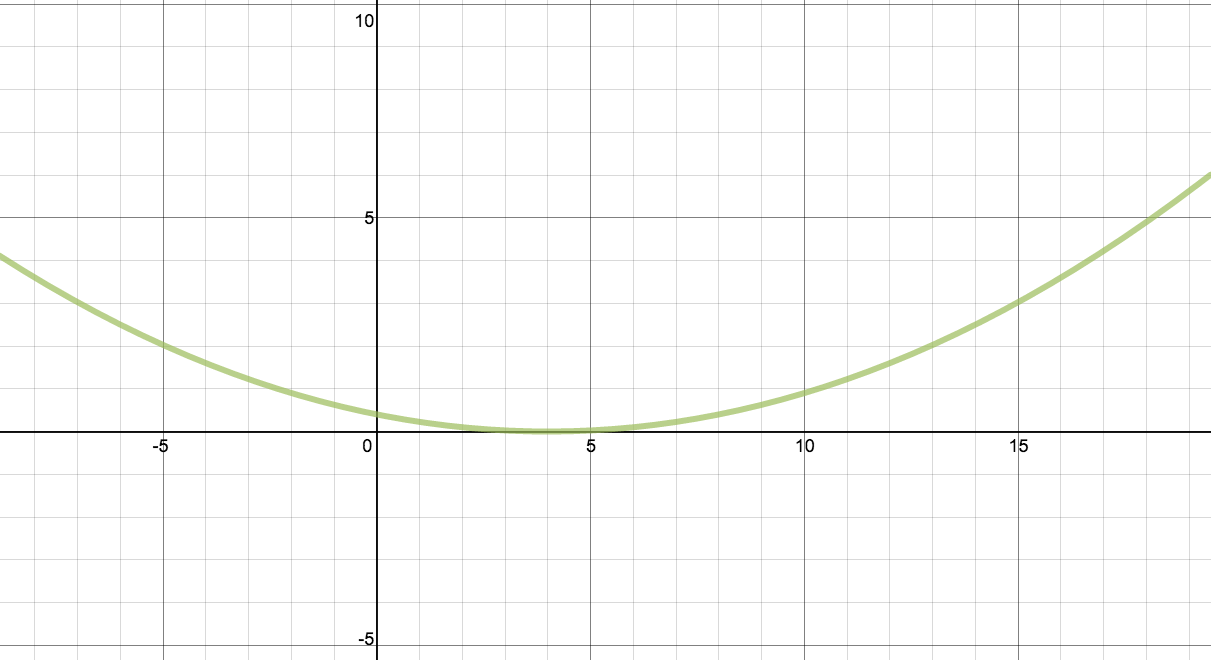
\includegraphics[width=0.900\linewidth]{smoluchowski.png}
\caption{Probability distribution with an attraction point.}\end{figure}

If we have some potential with a mininum point, then the motion of particles will be attracted to this minimum point. With the force in mind, we can write down the master equation, which is the $\zeta \neq 0$ case,
\begin{gather}
\begin{split}\frac{\partial}{\partial t} P(x,t) = \frac{\partial}{\partial x}\left( \frac{\partial U(x)}{\partial x} P(x,t)  \right) + D \frac{\partial^2}{\partial x^2} P(x,t) .\end{split}\notag\\\begin{split}\end{split}\notag
\end{gather}
This equation is called the Smoluchowski equation.

A very simple case is
\begin{gather}
\begin{split}\frac{\partial}{\partial t} P(x,t) = \gamma \frac{\partial}{\partial x}\left(x P(x,t)  \right) + D \frac{\partial^2}{\partial x^2} P(x,t) .\end{split}\notag\\\begin{split}\end{split}\notag
\end{gather}
which corresponds to a quadrople potential $U(x) = \gamma x^2/2$.

\begin{notice}{hint}{Hint:}
We have \DUspan{highlit}{methods of characteristics} to solve such partial differential equations.
\end{notice}

We can also use Fourier transform to solve the problem. However, we will only get
\begin{gather}
\begin{split}\frac{\partial}{\partial t} P^k = \cdots \frac{\partial}{\partial k} P^k  + \cdots k^2 P^k\end{split}\notag\\\begin{split}\end{split}\notag
\end{gather}
and the propagator is
\begin{gather}
\begin{split}\Pi(x,x',t) = \frac{e^{-(x - x' \exp(-\gamma t))^2}{4D\mathscr T(t)} }{\sqrt{4 \pi D \mathscr T(t)}}\end{split}\notag\\\begin{split}\end{split}\notag
\end{gather}
where $\mathscr T(t) = \frac{1-e^{-2\gamma t}}{2\gamma}$.
\begin{figure}[htbp]
\centering
\capstart

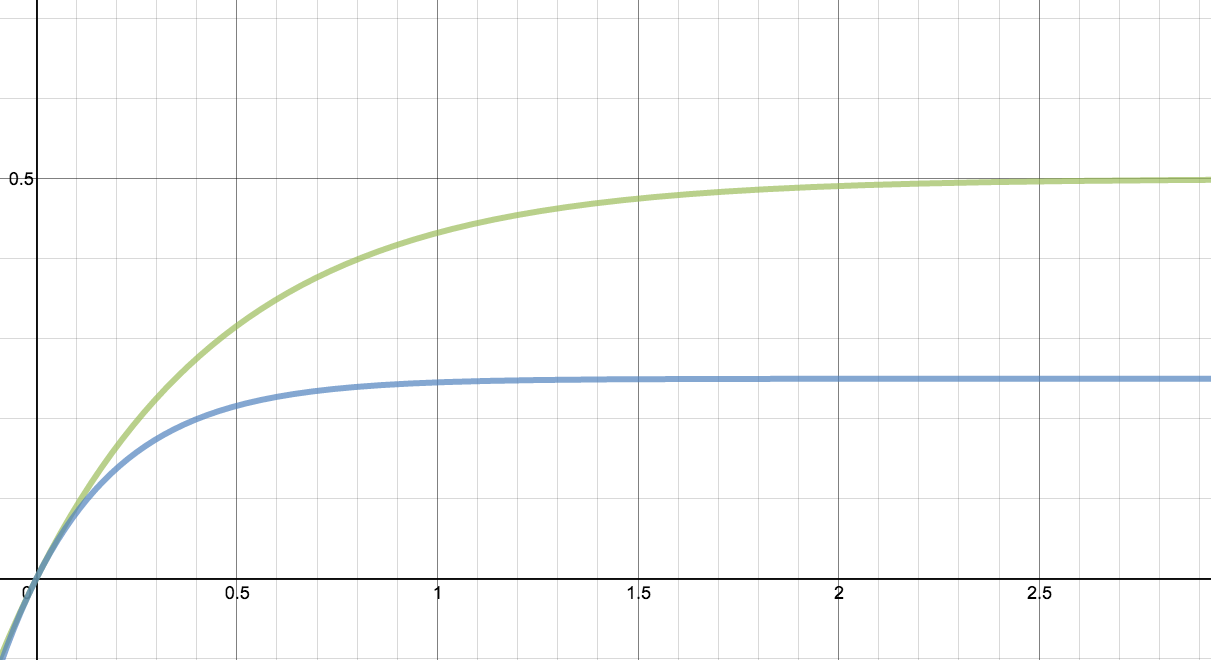
\includegraphics[width=0.900\linewidth]{smoluTime.png}
\caption{The redefined time parameter in the solution of Smoluchowski equation example.}\end{figure}


\subsection{Effect of Defects}
\label{nonequilibrium/effectOfDefects:effect-of-defects}\label{nonequilibrium/effectOfDefects::doc}
\index{Defect}

\subsubsection{Defects}
\label{nonequilibrium/effectOfDefects:index-0}\label{nonequilibrium/effectOfDefects:defects}
{\hfill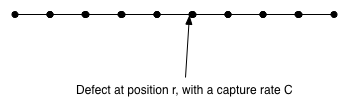
\includegraphics{effectsofDefects.png}\hfill}

A chain might have defects where the site captures the walker with a rate C. We would have a master equation of this kind
\begin{gather}
\begin{split}\frac{d}{dt}P_m = F(P_{m+1}+P_{m-1}-2P_m) - C \delta_{m,r} P_m .\end{split}\notag\\\begin{split}\end{split}\notag
\end{gather}
Consider an equation
\begin{gather}
\begin{split}\frac{d}{dt}y+\alpha y = f(t)\end{split}\notag\\\begin{split}\end{split}\notag
\end{gather}\begin{enumerate}
\item {} 
Solution to the equation when $\alpha$ is a constant is
\begin{gather}
\begin{split}y(t)  = e^{-\alpha t} y(0) + \int_0^t dt' e^{-\alpha (t - t')} f(t')\end{split}\notag\\\begin{split}\end{split}\notag
\end{gather}
\item {} 
$\alpha$ can be time dependent, instead of the expential term, we have $e^{-\int_{t'}^t ds \alpha(s)}$ as the Green function.

\end{enumerate}

\begin{notice}{warning}{Warning:}
Review Green function and Laplace transform.

General solution to first order differential equation is
\begin{gather}
\begin{split}y(t) = G(t,t_0) y(t_0) + \int_{t_0}^{t} df' G(t,t') f(t')\end{split}\notag\\\begin{split}\end{split}\notag
\end{gather}
If $\alpha$ is constant, use Laplace transform. Otherwise use Green function.
\end{notice}

\begin{notice}{hint}{Hint:}
Suppose we have a first order inhomogeneous differential equation with homogeous initial condition
\begin{gather}
\begin{split}L[y]\equiv \dot y + \alpha(t)y = f(t), \qquad \text{for } a < t, \qquad y(a) = 0\end{split}\notag\\\begin{split}\end{split}\notag
\end{gather}
The solution to this ODE is
\begin{gather}
\begin{split}y = \int_a^\infty G(t\vert \xi)f (\xi) d\xi,\end{split}\notag\\\begin{split}\end{split}\notag
\end{gather}
in which Green function is defined as
\begin{gather}
\begin{split}L[G(t\vert \xi)] = \delta(t - \xi), \qquad \text{for } a < t, \qquad G(a\vert \xi) = 0.\end{split}\notag\\\begin{split}\end{split}\notag
\end{gather}
In this specific case, Green function is
\begin{gather}
\begin{split}G(x\vert \xi) = e^{-\int_\xi^x \alpha(t) dt} H(t - \xi) .\end{split}\notag\\\begin{split}\end{split}\notag
\end{gather}\end{notice}

\begin{notice}{hint}{Hint:}
As a comparison to Green function method (which is not very helpful in 1st order ODE), general solution to first order differential equation
\begin{gather}
\begin{split}\dot y + \alpha(t)y = f(t)\end{split}\notag\\\begin{split}\end{split}\notag
\end{gather}
is
\begin{gather}
\begin{split}y(t) = \frac{\int\mu(t) f(t) dt + C}{\mu(t)}\end{split}\notag\\\begin{split}\end{split}\notag
\end{gather}
where $\mu(t) := e^{\int \alpha(t') dt'}$.
\end{notice}

\begin{notice}{hint}{Hint:}
Green function method for second order inhomogeneous equation is here in vacabulary.
\end{notice}

\begin{notice}{hint}{Hint:}
Laplace transform is a transform of a function $f(t)$ to a function of $s$,
\begin{gather}
\begin{split}L[f(t)] = \int_0^\infty f(t) e^{ - s t} dt .\end{split}\notag\\\begin{split}\end{split}\notag
\end{gather}
Some useful properties:
\begin{enumerate}
\item {} 
$L[\frac{d}{dt}f(t)] = s L[f(t)] - f(0)$;

\item {} 
$L[\frac{d^2}{dt^2}f(t) = s^2 L[f(t)] - s f(0) - \frac{d f(0)}{dt}$;

\item {} 
$L[\int_0^t g(\tau) d\tau ] = \frac{L[f(t)]}{s}$;

\item {} 
$L[\alpha t] = \frac{1}{\alpha} L[s/\alpha]$;

\item {} 
$L[e^{at}f(t)] = L[f(s-a)]$;

\item {} 
$L[tf(t)] = - \frac{d}{ds} L[f(t)]$.

\end{enumerate}

Some useful results:
\begin{enumerate}
\item {} 
$L[1] = \frac{1}{s}$;

\item {} 
$L[\delta] = 1$;

\item {} 
$L[\delta^k] = s^k$;

\item {} 
$L[t] = \frac{1}{s^2}$;

\item {} 
$L[e^{at}]= \frac{1}[s-a]$.

\end{enumerate}
\end{notice}

Suppose we have a time dependent source for master equation,
\begin{gather}
\begin{split}\frac{d}{dt}P_m = F(P_{m+1} + P_{m-1} - 2P_m) + g_m(t)\end{split}\notag\\\begin{split}\end{split}\notag
\end{gather}
The solution to this equation is
\begin{gather}
\begin{split}P_m(t) = \eta_m(t) + \int_0^t dt'\sum_n \Pi_{m-n}(t-t') g(t')\end{split}\notag\\\begin{split}\end{split}\notag
\end{gather}
Fourier transform of this solution
\begin{gather}
\begin{split}P^k(t) = \eta^k(t) + \int_0^t dt' \Pi^k(t-t') g^k(t')\end{split}\notag\\\begin{split}\end{split}\notag
\end{gather}
Then Laplace transform
\begin{gather}
\begin{split}\tilde P^k  = \tilde \eta^k + \tilde \Pi^k \tilde g^k  .\end{split}\notag\\\begin{split}\end{split}\notag
\end{gather}
\begin{notice}{warning}{Warning:}
\DUspan{highlit}{Laplace transform}
\end{notice}

Then we have in position space
\begin{gather}
\begin{split}\tilde P_m(\epsilon) = \tilde \eta_m(\epsilon)  + \sum_n \tilde \Pi_{m-n}(\epsilon) \tilde g_n(\epsilon)\end{split}\notag\\\begin{split}\end{split}\notag
\end{gather}
Now get back to our problem at the beginning.
\begin{gather}
\begin{split}\tilde g_n = - C\delta _{n,r} \tilde P_n\end{split}\notag\\\begin{split}\end{split}\notag
\end{gather}
The solution becomes
\begin{gather}
\begin{split}\tilde P_m = \tilde \eta _m - C \tilde \Pi_{m-r} \tilde P_r .\end{split}\notag\\\begin{split}\end{split}\notag
\end{gather}
We haven't solved it. The RHS depends on the probabillity. Notice that if we choose m=r, then
\begin{gather}
\begin{split}\tilde P_r  = \tilde \eta_r - C\tilde \Pi_0 \tilde P_r .\end{split}\notag\\\begin{split}\end{split}\notag
\end{gather}
So we can write down the rth component,
\begin{gather}
\begin{split}\tilde P_r = \frac{\tilde \eta_r}{1+C\tilde \Pi_0}  .\end{split}\notag\\\begin{split}\end{split}\notag
\end{gather}
Solution to the probability is
\begin{gather}
\begin{split}\tilde P_m &= \eta_m - C\tilde \Pi_{m-r}  \frac{\tilde \eta_r}{1+C\tilde \Pi_0} \\
& = \eta_m - \frac{\tilde \Pi_{m-r} \eta_r}{1/C + \tilde \Pi_0}\end{split}\notag\\\begin{split}\end{split}\notag
\end{gather}
The properties of this solution
\begin{enumerate}
\item {} 
$C\gg 1$, $\tilde \eta_m - \frac{\tilde \Pi_{m-r} \tilde \eta_r}{\tilde \Pi_0}$.

\item {} 
$C\ll 1$, $\tilde \eta_m$.

\end{enumerate}

\begin{notice}{warning}{Warning:}
We have to inverse using computer but why bother these transforms?
\end{notice}


\subsubsection{Survival Probability}
\label{nonequilibrium/effectOfDefects:survival-probability}\begin{gather}
\begin{split}Q(t) = \sum_n P_m(t)\end{split}\notag\\\begin{split}\end{split}\notag
\end{gather}
In our example,
\begin{gather}
\begin{split}\tilde Q(t) = \sum_m \tilde P_m = \frac{1}{\epsilon}\left( 1 - \frac{\tilde \eta_r}{1/C + \tilde \Pi_0} \right)\end{split}\notag\\\begin{split}\end{split}\notag
\end{gather}
Recall that Laplace transform gives us
\begin{gather}
\begin{split}\frac{d}{dt}Q \to \tilde Q - 1\end{split}\notag\\\begin{split}\end{split}\notag
\end{gather}
The survival probability can be written as
\begin{gather}
\begin{split}\frac{d}{dt} = - \int_0^t M(t-t') \eta(t').\end{split}\notag\\\begin{split}\end{split}\notag
\end{gather}

\subsubsection{Review of Effect of Defect}
\label{nonequilibrium/effectOfDefects:review-of-effect-of-defect}
A brief review:

Equation:
\begin{gather}
\begin{split}\frac{d}{dt} P_m = \text{Without Defect} - C \delta_{m,r} P_m\end{split}\notag\\\begin{split}\end{split}\notag
\end{gather}
Suppose we have the propagator as $\Pi_{m-n}(t,t_0)$. Laplace transform to solve it
\begin{gather}
\begin{split}\tilde P_m(\epsilon) = \tilde \eta_m(\epsilon) - C\tilde \Pi_{m-r}(\epsilon) \tilde P_r(\epsilon)\end{split}\notag\\\begin{split}\end{split}\notag
\end{gather}
By substitution of m with r, we find out
\begin{gather}
\begin{split}\tilde P_r(\epsilon) = \frac{\tilde \eta_m(\epsilon)}{1+ \tilde \Pi_0(\epsilon)}.\end{split}\notag\\\begin{split}\end{split}\notag
\end{gather}
Insert this result back to the solution, we can write donw the final result.
\begin{gather}
\begin{split}\tilde P_m(\epsilon) = \tilde \eta_m(\epsilon) - C\tilde \Pi_{m-r}(\epsilon) \tilde \eta_r(t) \frac{1}{1+C\tilde \Pi(\epsilon)}.\end{split}\notag\\\begin{split}\end{split}\notag
\end{gather}
Survival probability is defined as
\begin{gather}
\begin{split}Q(t) = \sum_m P_m .\end{split}\notag\\\begin{split}\end{split}\notag
\end{gather}
Then we can find out its Laplace transform, which is
\begin{gather}
\begin{split}\tilde Q(t) = \frac{1}{\epsilon} \left[ 1 - \frac{\tilde \eta_r(\epsilon)}{1/C + \tilde \Pi_0} \right]\end{split}\notag\\\begin{split}\end{split}\notag
\end{gather}
Looking through the table of Laplace transform, we know it's a transform of the time derivative of survival probability,
\begin{gather}
\begin{split}\frac{d}{dt}Q(t) = - \int_0^t dt' \mathscr M(t-t') \eta(t')\end{split}\notag\\\begin{split}\end{split}\notag
\end{gather}
in which
\begin{gather}
\begin{split}\mathscr M(t-t') = \frac{1}{1/C + \tilde \Pi_0} .\end{split}\notag\\\begin{split}\end{split}\notag
\end{gather}
\begin{notice}{hint}{Hint:}
The Laplace transform of propagator is
\begin{gather}
\begin{split}\tilde \Pi_0 = \int_0^\infty e^{-\epsilon t} \Pi_0 dt,\end{split}\notag\\\begin{split}\end{split}\notag
\end{gather}
which is actually decreasing when $\Pi_0$ is a constant.
\end{notice}

Take the limits to check the properties.
\begin{enumerate}
\item {} 
Motion limit is given by
\begin{gather}
\begin{split}\frac{1}{C} \ll \tilde \Pi_0 .\end{split}\notag\\\begin{split}\end{split}\notag
\end{gather}
The meaning of this is that the propagator decrease with time so fast that it becomes very small. In this limit, the survival probability is dominated by motion not the capture.

\item {} 
Capture limit,
\begin{gather}
\begin{split}\frac{1}{C} \gg \tilde \Pi_0 .\end{split}\notag\\\begin{split}\end{split}\notag
\end{gather}
In this limit, the survival probability is dominated by capture rate.

\end{enumerate}

\begin{notice}{hint}{Hint:}
This part is excerpted from the vocabulary part.

A very nice property of Laplace transform is
\begin{gather}
\begin{split}L_s [e^{at}f(t)] &= \int_0^\infty e^{-st} e^{-at} f(t) dt \\
& =  \int_0^\infty e^{-(s+a)t}f(t) dt \\
& = L_{s+a}[f(t)]\end{split}\notag\\\begin{split}\end{split}\notag
\end{gather}
which is very useful when dealing with master equations.

Two useful results are
\begin{gather}
\begin{split}L[I_0(2Ft)] = \frac{1}{\sqrt{ \epsilon^2 - (2F)^2 }}\end{split}\notag\\\begin{split}\end{split}\notag
\end{gather}
and
\begin{gather}
\begin{split}L[J_0[2Ft]]  = \frac{1}{\sqrt{\epsilon^2 + (2F)^2}},\end{split}\notag\\\begin{split}\end{split}\notag
\end{gather}
where $I_0(2Ft)$ is the modified Bessel functions of the first kind. $J_0(2Ft)$ is its companion.

Using the property above, we can find out
\begin{gather}
\begin{split}L[I_0(2Ft)e^{-2Ft}]  = \frac{1}{\sqrt{(\epsilon + 2F)^2 - (2F)^2}} .\end{split}\notag\\\begin{split}\end{split}\notag
\end{gather}\end{notice}


\subsubsection{Photosynthesis}
\label{nonequilibrium/effectOfDefects:photosynthesis}\begin{figure}[htbp]
\centering
\capstart

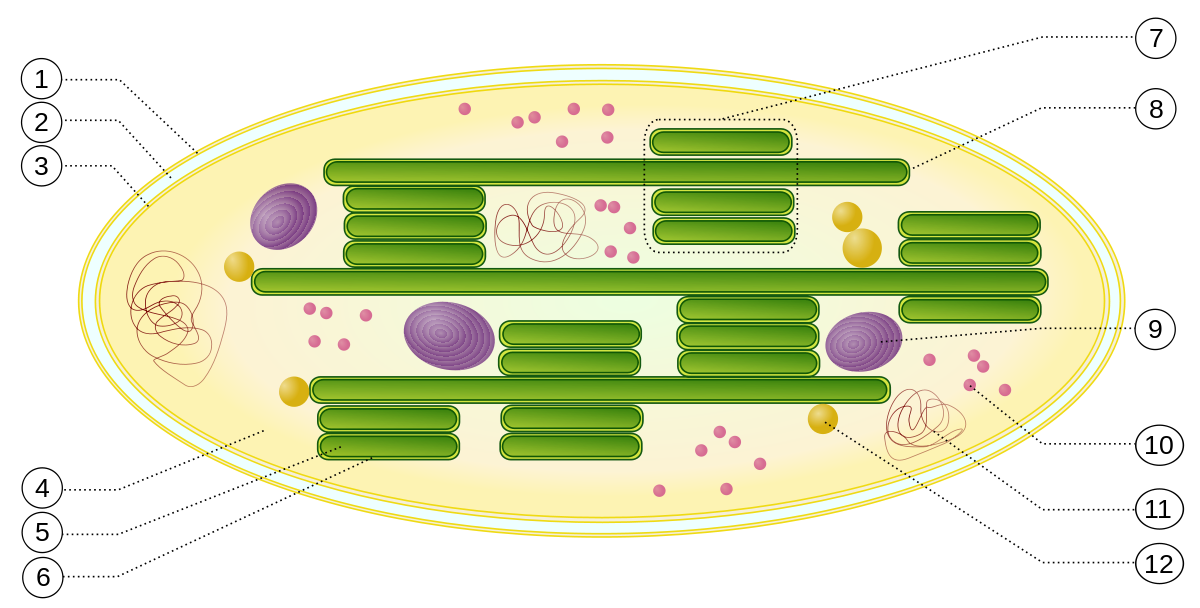
\includegraphics{chloroplast.png}
\caption{Captions are \href{https://en.wikipedia.org/wiki/Photosynthesis\#mediaviewer/File:Chloroplast.svg}{here on wikipedia}. Chloroplast ultrastructure: 1. outer membrane 2. intermembrane space 3. inner membrane (1+2+3: envelope) 4. stroma (aqueous fluid) 5. thylakoid lumen (inside of thylakoid) 6. thylakoid membrane 7. granum (stack of thylakoids) 8. thylakoid (lamella) 9. starch 10. ribosome 11. plastidial DNA 12. plastoglobule (drop of lipids)}\end{figure}

The obsorbed energy of photons is random walking in the chloroplast until it hit on a reaction center. Besides that, the photons can be emited after some time. So the process can be descibed with the following master equation.
\begin{gather}
\begin{split}\frac{d}{dt} P_m = \text{Without reaction and emission} - C\delta_{m,r} P_m - \frac{P_m}{\tau}\end{split}\notag\\\begin{split}\end{split}\notag
\end{gather}
where the last term is the emission term.

What experimentalists interest is the quantity called \DUspan{highlit}{quantum yield}, which is defined in the following way:
\begin{gather}
\begin{split}\text{quantum yield} & = \frac{\text{ Number of excitations in the trap or reaction center } }{\text{Number of total excitations}}\\
& = \frac{\text{Integration of survival probability with the reaction center}}{\text{Integration of survival probability without the raction center}} .\end{split}\notag\\\begin{split}\end{split}\notag
\end{gather}
We know that without the reaction,
\begin{gather}
\begin{split}\frac{d}{dt}Q + \frac{Q}{\tau} = 0\end{split}\notag\\\begin{split}\end{split}\notag
\end{gather}
so
\begin{gather}
\begin{split}Q(t) = Q(0) e^{-t/\tau}.\end{split}\notag\\\begin{split}\end{split}\notag
\end{gather}
Do the integration,
\begin{gather}
\begin{split}\frac{1}{\tau} \int_0^\infty Q(t) dt = 1 .\end{split}\notag\\\begin{split}\end{split}\notag
\end{gather}
The quantum yield is
\begin{gather}
\begin{split}\text{quantum yield} = \frac{\frac{1}{\tau} \int_0^\infty dt Q(t) \vert_{\text{with traps}} }{\frac{1}{\tau} \int_0^\infty dt Q(t) \vert_{\text{without traps}} } .\end{split}\notag\\\begin{split}\end{split}\notag
\end{gather}
The problem becomes the derivation of the two survival probabilities. However, we don't need the inverse Laplace transform because
\begin{gather}
\begin{split}\int_0^\infty Q(t) dt = L_{\epsilon=0}[Q(t)] .\end{split}\notag\\\begin{split}\end{split}\notag
\end{gather}
Let's define the quantities without traps to be with a prime. Notice that if we define a new quantity
\begin{gather}
\begin{split}\bar P_m = e^{t/\tau} P_m'\end{split}\notag\\\begin{split}\end{split}\notag
\end{gather}
because if we plugin it into the master equation, we will get back to the case without emission. Then we the solution immediately.
\begin{gather}
\begin{split}\bar P_m = P_m.\end{split}\notag\\\begin{split}\end{split}\notag
\end{gather}
So the survival probability with traps is
\begin{gather}
\begin{split}Q' = e^{-t/\tau} Q.\end{split}\notag\\\begin{split}\end{split}\notag
\end{gather}
This means that
\begin{gather}
\begin{split}\int_0^\infty Q'(t) dt &= \int_0^\infty e^{-t/\tau} Q(t) dt \\
& = L_{\epsilon=1/\tau} [Q(t)].\end{split}\notag\\\begin{split}\end{split}\notag
\end{gather}
This result simplifies our calculation so much because we don't need to calculate the survival probability in the case of traps. What we do is to use the Laplace transform of $Q(t)$ and set different $\epsilon$.

In details,
\begin{gather}
\begin{split}\tilde Q(\epsilon) = \frac{1}{\epsilon} \left( 1- \frac{\tilde \eta}{1/C + 1/\sqrt{\epsilon(\epsilon +4F)}} \right).\end{split}\notag\\\begin{split}\end{split}\notag
\end{gather}
So
\begin{gather}
\begin{split}\frac{1}{\tau}\int_0^\infty dt Q(t)  &= L_{\epsilon=0}[Q(t)] = \tilde Q(\epsilon=0) \\
\frac{1}{\tau}\int_0^\infty dt Q'(t)  &= L_{\epsilon=1/\tau}[Q'(t)] = \tilde Q(\epsilon=\frac{1}{\tau}).\end{split}\notag\\\begin{split}\end{split}\notag
\end{gather}
Then put $\tilde \eta (\epsilon) = \tilde \Pi_{m-r}(\epsilon) P_m(0)$ .


\subsubsection{Multiple Defects}
\label{nonequilibrium/effectOfDefects:multiple-defects}
We can solve for finite defects in principle. For example the two defects case should give us the following master equation
\begin{gather}
\begin{split}\frac{d}{dt}P_m = \cdots - C_r\delta_{m,r}P_m  - C_s \delta_{m,s} P_m.\end{split}\notag\\\begin{split}\end{split}\notag
\end{gather}
By using the two special cases that $m=r$ and $m=s$, we get two equations about $\tilde P_r$ and $\tilde P_s$,
\begin{gather}
\begin{split}\tilde P_r &= \eta_r - C_r \tilde \Pi_0 \tilde P_r - C_s \tilde \Pi_{r-s} \tilde P_r \\
\tilde P_s = \eta_s - C_r \tilde \Pi_{s-r} \tilde P_s - C_s \tilde \Pi_0 \tilde P_s.\end{split}\notag\\\begin{split}\end{split}\notag
\end{gather}
However, the problem gets very complicated as the number of defects becomes very large.


\subsection{Quantum Master Equation}
\label{nonequilibrium/quantumMasterEqn:quantum-master-equation}\label{nonequilibrium/quantumMasterEqn::doc}
The game of quantum master equations is presented in this lecture notes.


\subsubsection{Quantum Master Equation}
\label{nonequilibrium/quantumMasterEqn:id1}
\begin{notice}{important}{Important:}
In quantum mechanics, probability is not complete. We need density matrix.
\end{notice}

Quantum mechanics observables are averaging over all density matrix elements,
\begin{gather}
\begin{split}\langle O \rangle = \sum_{m,n} O_{nm}\rho_{mn}.\end{split}\notag\\\begin{split}\end{split}\notag
\end{gather}
For diagonalized density matrix, this averaging becomes the ordinary probability averaging.

However, even if we start with a diagonalized density matrix, the averaging procedure won't stay on the classical averaging procedure as time goes on. Off diagonal elements can be created out of the diagonal elements.

In that sense, it's not even possible to use the classical master equation to solve most quantum problems. We need the quantum master equation.

The first principle of quantum mechanics is
\begin{gather}
\begin{split}i\hbar \frac{d}{dt}\hat \rho = [\hat H,\hat \rho] = \hat L \hat \rho.\end{split}\notag\\\begin{split}\end{split}\notag
\end{gather}
Then the question is, as the first idea, how to derive an equation for the probability.


\paragraph{Pauli's Mistake}
\label{nonequilibrium/quantumMasterEqn:pauli-s-mistake}
Pauli derived the first quantum master equation which is not quite right.

The solution to a quantum system is
\begin{gather}
\begin{split}\hat \rho(t) = e^{-iL(t-t_0)} \hat \rho(t_0) .\end{split}\notag\\\begin{split}\end{split}\notag
\end{gather}
In Heisenberg picture,
\begin{gather}
\begin{split}\hat \rho(t+\tau) = e^{-i\tau \hat H} \hat \rho(t) e^{i\tau \hat H} .\end{split}\notag\\\begin{split}\end{split}\notag
\end{gather}
The diagonal elements of density matrix are
\begin{gather}
\begin{split}\rho_{mm}(t+\tau) = \bra{m}e^{-i\tau \hat H} \hat \rho(t) e^{i\tau \hat H} \ket{m}.\end{split}\notag\\\begin{split}\end{split}\notag
\end{gather}
The left hand side is the probability, $P_m$. Right had side becomes
\begin{gather}
\begin{split}\text{RHS} = \sum_{n,l}\bra{m}e^{-i\tau \hat H} \ket{n} \bra{n}\hat \rho(t) \ket{l}\bra{l} e^{i\tau \hat H} \ket{m}.\end{split}\notag\\\begin{split}\end{split}\notag
\end{gather}
Here is where Pauli's idea comes in. He assumed that the system is dirty enought to have repeatedly recurance of diagonalized density matrix. Then he use diagonalized density matrix to calculate the probability,
\begin{gather}
\begin{split}P_m(t+\tau) &= \sum_{n}\bra{m}e^{-i\tau \hat H} \ket{n} \bra{n}\hat \rho(t) \ket{n}\bra{n} e^{i\tau \hat H} \ket{m} \\
& = \sum_{n} P_n \left\vert \bra{m} e^{-i\tau \hat H} \ket{n}  \right\vert^2 .\end{split}\notag\\\begin{split}\end{split}\notag
\end{gather}
The term $\left\vert \bra{m} e^{-i\tau \hat H} \ket{n}  \right\vert^2$ RHS is the probability of a state n to be at state m after a short time $\tau$. We'll define this as $Q_{mn}(\tau)$.

So in short the probability is
\begin{gather}
\begin{split}P_m(t+\tau) = \sum_n Q_{mn}(\tau)P_n(t).\end{split}\notag\\\begin{split}\end{split}\notag
\end{gather}
Then we can repeat the Chapman method to derive a master eqution.

\begin{notice}{important}{Important:}
However, the Pauli assumption is basically the Fermi golden rule which requires a infinite amount of time. This is obviously not valid for an master equation system.
\end{notice}

Then it comes the van Hove derivation.


\paragraph{van Hove's Derivation}
\label{nonequilibrium/quantumMasterEqn:van-hove-s-derivation}
van Hove argued that Pauli's result is nonsense. He started with
\begin{gather}
\begin{split}P_m(t+\tau) &= \sum_n Q_{mn}(\tau) P_n(t) \\
P_m(t-\tau) & = \sum_n Q_{mn}(-\tau) P_m(t) .\end{split}\notag\\\begin{split}\end{split}\notag
\end{gather}
The key point is that $Q_{mn}(\tau) = Q_{mn}(-\tau)$,
\begin{gather}
\begin{split}Q_{mn}(\tau) & = \left\vert \bra{m} e^{-i\tau \hat H} \ket{n}  \right\vert^2 \\
& = \left\vert \bra{m} e^{i\tau \hat H} \ket{n}  \right\vert^2 \\
& = Q_{mn}(-\tau) .\end{split}\notag\\\begin{split}\end{split}\notag
\end{gather}
Without any calculations, we just know imediately that
\begin{gather}
\begin{split}P_m(t+\tau) = P_m(t-\tau) ,\end{split}\notag\\\begin{split}\end{split}\notag
\end{gather}
in other words, there's no evolution of probability density.


\subsubsection{van Hove}
\label{nonequilibrium/quantumMasterEqn:van-hove}
\begin{notice}{important}{Important:}
van Hove made a great progress by bringing up the following questions.
\begin{enumerate}
\item {} 
What systems can be described by master equations?

\item {} 
What's the time scale for quantum master equation to be valid?

\item {} 
How to derive a quantum master equation?

\end{enumerate}
\end{notice}

Suppose we have a quantum system with Hamiltonian,
\begin{gather}
\begin{split}\hat H = \hat H_0 + \lambda(t)\hat W .\end{split}\notag\\\begin{split}\end{split}\notag
\end{gather}
van Hove's idea was that quantum master equations can describe systems with diagonal singularity conditions.

Then he said, the time scale of the system should be long enough, the perturbation should be as small as the condition $\lambda^2 t \approx \text{constant}$.

\begin{notice}{warning}{Warning:}
This looks weird to me because I can not see why this is good for an approximation.
\end{notice}

So we can write down the diagonal elements
\begin{gather}
\begin{split}P_m & = \bra{m}\hat \rho \ket{m} \\
& = \sum_{m,n} \bra{m} e^{i\hat H t/\hbar} \ket{n}\bra{n} \hat \rho(0) \ket{l}\bra{l} e^{-iHt/\hbar} \ket{m} \\
& = \sum_{m,n} \left\vert \bra{m} e^{i (\hat H_0 + \lambda \hat W) t/\hbar } \ket{n} \right\vert^2 \rho_{nl}(0) .\end{split}\notag\\\begin{split}\end{split}\notag
\end{gather}
van Hove applied random phase condition for only initial condition, $\rho_{nl}(0)$ is diagonalized at initial $t=0$.

Then we have
\begin{gather}
\begin{split}\rho_{nl} (0) = \rho_{nn} \delta_{nl} = P_n(0) \delta_{nl} .\end{split}\notag\\\begin{split}\end{split}\notag
\end{gather}
Put this result back to the probability,
\begin{gather}
\begin{split}P_m = \sum_n \left\vert \bra{m} e^{i (\hat H_0 + \lambda \hat W) t/\hbar } \ket{n} \right\vert^2 P_n(0) .\end{split}\notag\\\begin{split}\end{split}\notag
\end{gather}
Then use the whole Dyson series then selectively make some terms zero and use the assumptions to derive a master equation.


\subsubsection{Zwawzig and Nakajiwa}
\label{nonequilibrium/quantumMasterEqn:zwawzig-and-nakajiwa}
They invented the projection technique.

First of all define a diagonalizing operator $\hat D$ which just keeps the diagonal elements and simply drops the off diagonal elements. We see that $1-\hat D$ will element all diagonal elements.

We can define the diagonalized density matrix as $\hat \rho_d = \hat D \hat \rho$ and off-diagonalized density matrix as $\hat \rho_{od} = (1-\hat D)\hat \rho$. As an application,
\begin{gather}
\begin{split}\hat \rho = \hat \rho_d + \hat \rho_{od} .\end{split}\notag\\\begin{split}\end{split}\notag
\end{gather}
Starting from the von Neumann equation,
\begin{gather}
\begin{split}i\hbar \partial_t \hat \rho = \left[\hat H, \hat \rho \right] .\end{split}\notag\\\begin{split}\end{split}\notag
\end{gather}
By using the Liouville operator,
\begin{gather}
\begin{split}\partial_t \hat \rho = -i \hat L \hat \rho .\end{split}\notag\\\begin{split}\end{split}\notag
\end{gather}
Apply $\hat D$ and $1-\hat D$ to the von Neumann equation,
\begin{gather}
\begin{split}\partial_t \hat \rho_d & = -i \hat D  \hat L \hat \rho \\
\partial_t \hat \rho _{od} & = -i (1 - \hat D)  \hat L \hat \rho .\end{split}\notag\\\begin{split}\end{split}\notag
\end{gather}
Use the relation that $\hat \rho = \hat \rho_d + \hat \rho_{od}$, we have
\begin{gather}
\begin{split}\partial_t \hat \rho_d & = -i \hat D  \hat L \hat \rho_d - i \hat D  \hat L \hat \rho _ {od} \\
\partial_t \hat \rho _{od} & = - i (1 - \hat D)  \hat L \hat \rho _ d - i (1 - \hat D)  \hat L \hat \rho_{od}  .\end{split}\notag\\\begin{split}\end{split}\notag
\end{gather}
Solve the second equation using Green function technique,
\begin{gather}
\begin{split}\hat \rho_{od} = e^{-i(1-\hat D)\hat L t} + \int_0^t dt' e^{-i(1-\hat D) \hat L (t-t')}(-i(1-\hat D)\hat L \hat \rho_d(t')) .\end{split}\notag\\\begin{split}\end{split}\notag
\end{gather}
\begin{notice}{hint}{Hint:}
Recall that the solution for
\begin{gather}
\begin{split}\dot y + \alpha y = f\end{split}\notag\\\begin{split}\end{split}\notag
\end{gather}
is
\begin{gather}
\begin{split}y = e^{-\alpha t} y(0) + \int_0^t dt' e^{-\alpha (t-t')} f(t') .\end{split}\notag\\\begin{split}\end{split}\notag
\end{gather}\end{notice}

Insert this solution to the equation of $\hat \rho_d$,
\begin{gather}
\begin{split}{\color{red}\partial_t \hat \rho_d = - i\hat D\hat L \hat \rho_d -  \hat D\hat L \int_0^t dt' e^{-i(1-\hat D) \hat L (t-t')}(1-\hat D)\hat L \hat \rho_d(t')} {\color{blue} - i \hat D \hat L e^{-i(1-\hat D)\hat L t} \rho_{od}(0) }.\end{split}\notag\\\begin{split}\end{split}\notag
\end{gather}
What happened to the blue term? It disapears when we apply the initial random phase condition.

When it happens we get our closed master equation for $\hat \rho_d$, which is an equation for the probability.


\subsubsection{About Off-diagonal Elements}
\label{nonequilibrium/quantumMasterEqn:about-off-diagonal-elements}
Though we need to set $\rho_{od}(0)=0$ to have a closed master equation, that doens't mean we have to make only localized initial condition on only one state.
\begin{quote}

``We can always use phasers.''

\begin{flushright}
---V. M. Kenkre
\end{flushright}
\end{quote}

Suppose we have a system with five possible states, the off-diagonal elements don't exist initially if the system is in only one state.

{\hfill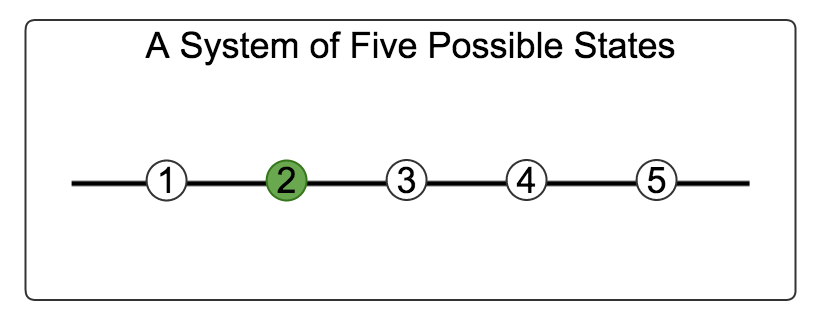
\includegraphics{quantum1state.png}\hfill}

The density matrix will contain off-diagonal elements if we have two states initially.

{\hfill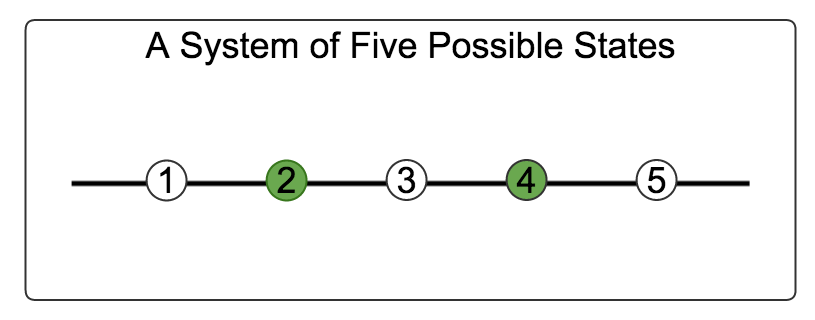
\includegraphics{quantum2states.png}\hfill}

However, we can always choose a combination of the states to use as the basis, so that the density matrix becomes diagonalized.


\subsubsection{Simplify Quantum Master Equation}
\label{nonequilibrium/quantumMasterEqn:simplify-quantum-master-equation}
We derived some sort of quantum master equation using projection method. Here we will simplify it.

Let's stare at the results for a minute.
\begin{gather}
\begin{split}{\color{red}\partial_t \hat \rho_d = - i\hat D\hat L \hat \rho_d -  \hat D\hat L \int_0^t dt' e^{-i(1-\hat D) \hat L (t-t')}(1-\hat D)\hat L \hat \rho_d(t')} {\color{blue} - i \hat D \hat L e^{-i(1-\hat D)\hat L t} \rho_{od}(0) }.\end{split}\notag\\\begin{split}\end{split}\notag
\end{gather}
By definition, $\rho_d=\hat D\rho$. So what is $\hat D \hat L \rho_d$?
\begin{gather}
\begin{split}\hat D \hat L \rho_d & = \hat D\hat L \hat D \hat \rho \\
& = \hat D \left[ {\color{magenta}  \begin{pmatrix}\rho_{11} & 0 & 0 & \cdots \\ 0 & \rho_{22} & 0 & \cdots \\ 0 & 0 & \rho_{33} & \cdots  \\ \vdots & \vdots & \vdots &  \ddots  \end{pmatrix} \begin{pmatrix} H_{11} & H_{12} & H_{13} & \cdots \\ H_{21} & H_{22} & H_{23} & \cdots  \\ H_{31} & H_{32} & H_{33} & \cdots \\ \vdots & \vdots \vdots & & \ddots \end{pmatrix}    } -  {\color{green} \begin{pmatrix} H_{11} & H_{12} & H_{13} & \cdots \\ H_{21} & H_{22} & H_{23} & \cdots  \\ H_{31} & H_{32} & H_{33} & \cdots \\ \vdots & \vdots \vdots & & \ddots   \end{pmatrix} \begin{pmatrix} \rho_{11} & 0 & 0 & \cdots \\ 0 & \rho_{22} & 0 & \cdots \\  0 & 0 & \rho_{33} & \cdots \\ \vdots & \vdots & \ddots & \cdots \end{pmatrix} } \right]\end{split}\notag\\\begin{split}\end{split}\notag
\end{gather}
We can easily see that the diagonal elements are equal for the two terms (magenta and green) in the braket so all the diagonal elements go away. Now when the $\hat D$ outside of the bracket applied, the whole term is zero.

We are so lucky to eliminate the term $-i\hat D\hat L\hat \rho_d$.

We do perturbation theory most of the time. Consider the case that Hamiltonian of the system is $\hat H = \hat H_0 + \lambda \hat W$. We can split the Liouville operator into two parts, :math:{\color{red}\bfseries{}{}`}hat L = hat L\_0 + lambda hat L\_W {\color{red}\bfseries{}{}`}.

Our master equation becomes
\begin{gather}
\begin{split}\partial_t \hat \rho_d & =  -  \int_0^t dt' \hat D (\hat L_0 + \lambda \hat L_W ) e^{-i(1-\hat D) (\hat L_0 + \lambda \hat L_W  )(t-t')}(1-\hat D)\hat L \hat \rho_d \\
& =  -  \int_0^t dt' \hat D (\hat L_0 + \lambda \hat L_W ) e^{-i(1-\hat D)  (\hat L_0 + \lambda \hat L_W ) (t-t')} (\hat L_0 + \lambda \hat L_W ) \hat \rho_d \\
& =  -  \int_0^t dt' \mathscr K(t-t') \hat \rho_d .\end{split}\notag\\\begin{split}\end{split}\notag
\end{gather}
in which $- i \hat D \hat L e^{-i(1-\hat D)\hat L t} \rho_{od}(0) = 0$ (initial condition), $\hat D \hat L \rho_d = 0$ (just proved).

We have the definition
\begin{gather}
\begin{split}\mathscr K(t-t') & = \hat D (\hat L_0 + \lambda \hat L_W ) e^{-i(1-\hat D)  (\hat L_0 + \lambda \hat L_W ) (t-t')} (\hat L_0 + \lambda \hat L_W ) .\end{split}\notag\\\begin{split}\end{split}\notag
\end{gather}
In weak coupling interaction, $\lambda \rightarrow 0$, we can put $\lambda = 0$ in the exponential.
\begin{gather}
\begin{split}\mathscr K(t-t')  &=  \hat D (\hat L_0 + \lambda \hat L_W ) e^{-i(1-\hat D)  (\hat L_0 + \lambda \hat L_W ) (t-t')} (\hat L_0 + \lambda \hat L_W )  \\
&= \hat D (\hat L_0 + \lambda \hat L_W ) e^{-i(1-\hat D)  \hat L_0 (t-t')} (\hat L_0 + \lambda \hat L_W ) \\
&= \hat D \hat L_0  e^{-i(1-\hat D)  \hat L_0 (t-t')} \hat L_0  + \lambda \hat D \hat L_0  e^{-i(1-\hat D)  \hat L_0 (t-t')}   \hat L_W   \\
\phantom{\mathscr K(t-t')} & \phantom{{} = } + \lambda \hat D  \hat L_W  e^{-i(1-\hat D)  \hat L_0 (t-t')} \hat L_0  + \lambda^2 \hat D   \hat L_W  e^{-i(1-\hat D)  \hat L_0 (t-t')}  \hat L_W  \\
&=  \lambda^2 \hat D   \hat L_W  e^{-i(1-\hat D)  \hat L_0 (t-t')}  \hat L_W  \\
&=  \lambda^2 \hat D   \hat L_W  e^{-i\hat L_0 (t-t')}  \hat L_W  .\end{split}\notag\\\begin{split}\end{split}\notag
\end{gather}
I dropped several terms even the first order of $\lambda$. This has been done correctly because the interaction term can be very different from the zeroth order. \footnote{
Refer to \emph{Quantum Noise} by Gardiner and Zoller, Chapter 5, Section 1.
}

With a lot of terms being disappears, we can now start to look at the numbers which ia the density matrix elements sandwiched between states,
\begin{gather}
\begin{split}\bra{m} \partial_t \rho_d \ket{m} = -\lambda^2 \bra{m} \int_0^t dt' \hat L_W e^{-i(t-t')\hat L_0} \hat L_W \rho_d(t') \ket{m}.\end{split}\notag\\\begin{split}\end{split}\notag
\end{gather}
\begin{notice}{hint}{Hint:}
Here is an useful relation,
\begin{gather}
\begin{split}e^{iA\hat L} \hat O & = \hat O + i A \hat L \hat O + \frac{(iA)^2}{2} \hat L \hat L \hat O + \cdots \\
& = \hat O + iA[\hat H, \hat O] + \frac{(iA)^2}{2}  [\hat H, [\hat H,\hat O]] + \cdots \\
& = e^{iA\hat H}\hat O e^{-iA\hat H}\end{split}\notag\\\begin{split}\end{split}\notag
\end{gather}\end{notice}

Notice that $\hat L_W \hat \rho_d = \frac{1}{\hbar}[W, \rho_d]$. Define $\hat{\mathscr M} = e^{-i(t-t')\hat H_0}[\hat V,\hat \rho_d]e^{i(t-t')\hat H_0}$.
\begin{gather}
\begin{split}\bra{m} \partial_t \rho_d \ket{m} &= -\lambda^2 \bra{m} \int_0^t dt' [\hat W, e^{-i(t-t')\hat L_0}[\hat W, \rho_d(t')]] \ket{m}  \\
& = -\lambda^2 \bra{m} \int_0^t [\hat W, ] dt' \ket{m}  \\
& = -\lambda^2 \left( \bra{m} \int_0^t dt' \hat W\hat{\mathscr M} \ket{m} - \bra{m} \int_0^t \hat{\mathscr M}\hat W\ket{m} dt' \right) \\
& = -\lambda^2 \int_0^t dt' \left( \bra{m} \hat W\hat{\mathscr M} \ket{m} - \bra{m} \hat{\mathscr M}\hat W\ket{m}  \right) \\
& = -\lambda^2 \int_0^t dt' \sum_n (W_{mn}\mathscr M_{nm} - \mathscr M_{mn}W_{nm}).\end{split}\notag\\\begin{split}\end{split}\notag
\end{gather}
We know that $\rho_d = P_{m}$. So the master equation becomes
\begin{gather}
\begin{split}\partial_t P_m(t) = -\lambda^2 \int_0^t dt' \sum_n (W_{mn}\mathscr M_{nm} - \mathscr M_{mn}W_{nm}).\end{split}\notag\\\begin{split}\end{split}\notag
\end{gather}
The eigen function of the system is
\begin{gather}
\begin{split}\hat H_0 \ket{m} = \epsilon_m \ket{m} .\end{split}\notag\\\begin{split}\end{split}\notag
\end{gather}
With this result we can calculate the matrix elements,
\begin{gather}
\begin{split}\mathscr M_{mn} &= \bra{m} e^{-i(t-t')\hat H_0}[\hat W,\hat \rho_d]e^{i(t-t')\hat H_0} \ket{n} \\
& = e^{-i(t-t')\epsilon_m} \bra{m} [\hat W, \hat \rho_d] \ket{n} e^{i(t-t')\epsilon_n} \\
& = \sum_\mu e^{-i(t-t')\epsilon_m} (\bra{m} \hat W \ket{\mu} \bra{\mu} \hat \rho_d \ket{n} - \bra{m} \hat \rho_d \ket{\mu}\bra{\mu} \hat W \ket{n} )e^{i(t-t')\epsilon_n} \\
& = \sum_\mu  e^{-i(t-t')\epsilon_m} (W_{m\mu}\rho_{\mu n} - \rho_{m\mu}W_{\mu n}) e^{i(t-t')\epsilon_n} \\
& = e^{-i(t-t')\epsilon_m} ( W_{mn}P_{n} - P_{m}W_{m n} ) e^{i(t-t')\epsilon_n} .\end{split}\notag\\\begin{split}\end{split}\notag
\end{gather}
Finally we have our quantum master equation,
\begin{gather}
\begin{split}\partial_t P_m &= -\lambda^2 \int_0^t dt' \sum_n \left[ ( W_{mn} e^{-i(t-t')\epsilon_n} ( W_{nm}P_{m} - P_{n}W_{n m} ) e^{i(t-t')\epsilon_m}) - (e^{-i(t-t')\epsilon_m} ( W_{mn}P_{n} - P_{m}W_{m n} ) e^{i(t-t')\epsilon_n} )W_{nm}  \right] \\
& =  -\lambda^2 \int_0^t dt' \sum_n \left[ ( W_{mn} e^{-i(t-t')(\epsilon_n - \epsilon_m )  }  W_{nm} (P_{m} - P_{n}) - (e^{-i(t-t')\epsilon_m} ( W_{mn}P_{n} - P_{m}W_{m n} ) e^{i(t-t')\epsilon_n} )W_{nm}  \right] \\
& = -2 \lambda^2 \int_0^t dt' \sum_n \left\vert W_{mn} \right\vert^2 \left[ P_n- P_m \right] \cos((\epsilon_m-\epsilon_n)(t-t'))\end{split}\notag\\\begin{split}\end{split}\notag
\end{gather}
which is actually the \DUspan{highlit}{Fermi's golden rule}.

Define $\Omega_{mn}(t-t')=\Omega_{nm}(t-t') = 2\lambda^2 \left\vert W_{mn} \right\vert^2\cos((t-t')(\epsilon_m-\epsilon_n))$, we can write the master equation into a really simple form,
\begin{gather}
\begin{split}\partial_t P_m = \int_0^t dt' \sum_n \left( \Omega_{mn}(t-t') P_n - \Omega_{nm}(t-t') P_m \right).\end{split}\notag\\\begin{split}\end{split}\notag
\end{gather}

\subsubsection{Markovian - Kenkre Approach}
\label{nonequilibrium/quantumMasterEqn:markovian-kenkre-approach}
We can simplify the equation more using Markovian approximation,
\begin{gather}
\begin{split}\Omega_{mn}(t) = \delta(t) \left[\int_0^t d\tau \Omega_{mn}(\tau) \right].\end{split}\notag\\\begin{split}\end{split}\notag
\end{gather}
We can see that the Laplace transform of this is really simple,
\begin{gather}
\begin{split}\tilde \Omega_{mn}(\epsilon) =  \Omega_{mn}(0).\end{split}\notag\\\begin{split}\end{split}\notag
\end{gather}
\begin{notice}{hint}{Hint:}
Laplace transform of integral and delta function are
\begin{gather}
\begin{split}\mathscr L (\delta(t-a)) &= e^{-a\epsilon}, \qquad \text{for } a>0. \\
\mathscr L (\int_0^t f(t') dt') & = \frac{1}{\epsilon} \mathscr L_\epsilon (f(t)).\end{split}\notag\\\begin{split}\end{split}\notag
\end{gather}
So we have the Laplace transform of $\Omega_{mn}(t) = \delta(t) \int_0^t d\tau \Omega_{mn}(\tau)$ on both sides,
\begin{gather}
\begin{split}\tilde \Omega_{mn}(\epsilon) & = \int_0^\infty dt e^{-\epsilon t}  \delta(t) \int_0^t d\tau \Omega_{mn}(\tau) \\
& = \int_0^\infty \frac{1}{-\epsilon}  \delta(t) \int_0^t d\tau \Omega_{mn}(\tau) d e^{-\epsilon t} \\
& = \frac{1}{\epsilon} \int_0^\infty   e^{-\epsilon t} d\left(\delta(t) \int_0^t d\tau \Omega_{mn}(\tau) \right)  \\
& = \frac{1}{\epsilon} \int_0^\infty   e^{-\epsilon t} \int_0^t d\tau \Omega_{mn}(\tau)   d\left(\delta(t) \right) + \frac{1}{\epsilon} \int_0^\infty   e^{-\epsilon t}  \delta(t)  d\left( \int_0^t d\tau \Omega_{mn}(\tau) \right)  \\
& = \frac{1}{\epsilon} \int_0^\infty   e^{-\epsilon t}  \delta(t) \Omega_{mn}(t)  dt  \\
& = \frac{1}{\epsilon}   \Omega_{mn}(0)\end{split}\notag\\\begin{split}\end{split}\notag
\end{gather}\end{notice}

\begin{notice}{warning}{Warning:}
Derive the Fermi's golden rule from this.
\end{notice}

Finally we can reach Fermi's golden rule.


\subsubsection{Markovian - Another Approach}
\label{nonequilibrium/quantumMasterEqn:markovian-another-approach}
\textbf{I'll put all the :math:{}`hbar{}`s back into the equations in this subsection.}

I read the Markovian idea on quantiki \footnote{
\href{http://www.quantiki.org/wiki/}{Quantiki} is a website of quantum information etc. The item about master equation is \href{http://www.quantiki.org/wiki/Master\_equation}{here} .
} . Here is my derivation of Fermi's golden rule from quantum master equation using this approach.

First of all, we can use interaction picture. Master equation here can be rewritten using interaction picture.
\begin{gather}
\begin{split}\partial_t P_m & =  -\lambda^2/\hbar^2 \int_0^t dt' \sum_n \left[ ( W_{mn} e^{-i(t-t')(\epsilon_n - \epsilon_m ) /\hbar }  W_{nm} (P_{m} - P_{n}) - (e^{-i(t-t')\epsilon_m/\hbar} ( W_{mn}P_{n} - P_{m}W_{m n} ) e^{i(t-t')\epsilon_n/\hbar} )W_{nm}  \right] \\
& = -\lambda^2/\hbar^2 \int_0^t dt' \sum_n \left[ ( e^{it\epsilon_m/\hbar}W_{mn} e^{-i t \epsilon_n/\hbar } e^{it'\epsilon_n/\hbar} W_{nm} e^{-it'\epsilon_m/\hbar} (P_{m} - P_{n}) - (e^{it\epsilon_m/\hbar}  W_{mn} e^{-it\epsilon_n/\hbar} (P_{n} - P_{m}) e^{it'\epsilon_n/\hbar} )W_{nm} e^{-it'\epsilon_m/\hbar} \right] \\
& = -\lambda^2/\hbar^2 \sum_n \left[  \int_0^t dt' W_{mn}^I W_{nm}^I(P_m-P_n) - \int_0^t dt' W_{mn}^I W_{nm}^I(P_n-P_m)  \right]\end{split}\notag\\\begin{split}\end{split}\notag
\end{gather}
Markovian means there is no dependence on the past, in other words, \textbf{the two point correlation in time} is non-zero only when the two time are equal in the correlation function, $\mathrm{Corr}(t_1,t_2)=0$ for all $t_1\not= t_2$. In our master equation case,
\begin{gather}
\begin{split}&\int_0^t dt' W_{mn}^I(t) W_{nm}^I(t')(P_m(t')-P_n(t')) \\
& = \int_0^t dt' W_{mn}^I(t-t') W_{nm}^I(0)(P_m(t)-P_n(t)) \\
& = (P_m(t)-P_n(t)) \lim_{t\rightarrow \infty}\int_0^t dt' W_{mn}^I(t-t') W_{nm}^I(0) .\end{split}\notag\\\begin{split}\end{split}\notag
\end{gather}
\begin{notice}{hint}{Hint:}
This is corresponding to the Kenkre definition of Markovian.
\end{notice}

So our master equation becomes
\begin{gather}
\begin{split}\partial_t P_m(t) &= -\frac{\lambda^2}{\hbar ^2} \sum_n(P_m - P_n) \left[ \lim_{t\rightarrow \infty} \left( \int_0^t dt' e^{i(t-t')\epsilon_m/\hbar} W_{mn} e^{-i(t-t')\epsilon_n/\hbar} W_{nm} + \int_0^t dt' e^{-i(t-t')\epsilon_m/\hbar} W_{mn} e^{i(t-t')\epsilon_n/\hbar} W_{nm} \right) \right] \\
& = -\frac{\lambda^2}{\hbar^2} \sum_n (P_m - P_n) \left[ \lim_{t\rightarrow \infty} \left( \frac{\left| W_{mn}\right|^2 }{i\omega_{nm}} \left( e^{-it\omega_{mn}}  - e^{it\omega_{mn}}  \right) \right)   \right] \\
& = -\frac{\lambda^2}{\hbar^2} \sum_n (P_m - P_n) \left[ 2\left| W_{mn}\right|^2  \lim_{t\rightarrow \infty}   \left( \frac{i\sin(\omega_{mn}t)}{i\omega_{nm}}   \right)   \right] \\
& =  \sum_n (P_m - P_n) \left[  \frac{2 \pi \lambda^2 \left| W_{mn}\right|^2 }{\hbar^2}  \lim_{t\rightarrow \infty}   \left( \frac{\sin(\omega_{mn}t)}{\pi\omega_{nm}}   \right)   \right]\end{split}\notag\\\begin{split}\end{split}\notag
\end{gather}
\begin{notice}{important}{Important:}
We have the following expression,
\begin{gather}
\begin{split}\lim_{\epsilon\rightarrow 0} \frac{\sin(x/\epsilon)}{\pi x} = \delta(x) .\end{split}\notag\\\begin{split}\end{split}\notag
\end{gather}\end{notice}

Using this expression of delta, we derived the Fermi's golden rule.
\begin{gather}
\begin{split}\partial_t P_m & =  \sum_n (P_m - P_n)   \frac{2 \pi \lambda^2 \left| W_{mn}\right|^2 }{\hbar^2}  \delta(\omega_mn)  \\
& =  \sum_n (P_m - P_n)   \frac{2 \pi \lambda^2 \left| W_{mn}\right|^2 }{\hbar^2}  \delta((\epsilon_m - \epsilon_n)/\hbar) \\
& =  \sum_n (P_m - P_n)   \frac{2 \pi \lambda^2 \left| W_{mn}\right|^2 }{\hbar}  \delta(\epsilon_m - \epsilon_n)\end{split}\notag\\\begin{split}\end{split}\notag
\end{gather}
Comparing this result with the classical master equation, we can find out the transition rate,
\begin{gather}
\begin{split}\Omega_{mn} = \frac{2 \pi \lambda^2 \left| W_{mn}\right|^2 }{\hbar}  \delta(\epsilon_m - \epsilon_n)\end{split}\notag\\\begin{split}\end{split}\notag
\end{gather}
which is exactly the Fermi's golden rule.


\subsubsection{Footnotes}
\label{nonequilibrium/quantumMasterEqn:footnotes}

\subsection{Brownian Motion}
\label{nonequilibrium/brownianMotion:brownian-motion}\label{nonequilibrium/brownianMotion::doc}
The equation for Brownian Motion is
\begin{gather}
\begin{split}\frac{d}{dt} v + \gamma v = R(t),\end{split}\notag\\\begin{split}\end{split}\notag
\end{gather}
where $R(t)$ is random force which requires
\begin{gather}
\begin{split}\avg{R(t)} &= 0 \\
\avg{R(t)R(t')} = C \delta(t-t') .\end{split}\notag\\\begin{split}\end{split}\notag
\end{gather}
This equation is the linear \DUspan{highlit}{Langevin equation}.

The formal solution, which seems to be useless, is
\begin{gather}
\begin{split}v(t) = v(0)e^{-\gamma t} + \int_0^t dt' e^{-\gamma (t-t')} R(t') .\end{split}\notag\\\begin{split}\end{split}\notag
\end{gather}
Knowing that $R(t)$ is random, or stochastic, we imediately realize that $v(t)$ is stochastic. The thing to do is to find out the statistics.

This quantity squared is,
\begin{gather}
\begin{split}v(t)^2 = v(0)^2 e^{-2\gamma t} + \int_0^t dt'\int_0^t dt'' e^{-\gamma (t- t')} e^{-\gamma (t - t'')} R(t')R(t'') + \mathrm{Cross Terms}\end{split}\notag\\\begin{split}\end{split}\notag
\end{gather}
Average of the solution is
\begin{gather}
\begin{split}\avg{v} &= \avg{v(0)e^{-\gamma t}} + {\color{magenta}\avg{\int_0^t dt' e^{-\gamma (t-t')} R(t') } } \\
\avg{v^2} &= \avg{v(0)^2 e^{-2\gamma t}} + \avg{\int_0^t dt'\int_0^t dt'' e^{-\gamma (t- t')} e^{-\gamma (t - t'')} R(t')R(t'')} + {\color{magenta}\avg{ \mathrm{Cross Terms}} }\end{split}\notag\\\begin{split}\end{split}\notag
\end{gather}
where these magenta colored terms are zero.

\begin{notice}{hint}{Hint:}
Note that the average here is ensemble average. Define probability density $P(v,t)$ for velocity at time t. Recall that in velocity space, Liouville equation is
\begin{gather}
\begin{split}\frac{d}{dt}P(v,t) + \frac{d}{dt}j = 0.\end{split}\notag\\\begin{split}\end{split}\notag
\end{gather}
It's very important to realize that this current density is the current density in velocity space. Applying $d_t v = -\gamma vt R(t)$,
\begin{gather}
\begin{split}\frac{d}{dt}P(v,t) + \frac{d}{dv} \left(  (-\gamma v+ R(t))P(v,t) \right) = 0 .\end{split}\notag\\\begin{split}\end{split}\notag
\end{gather}\end{notice}

\begin{notice}{warning}{Warning:}
Now I am curious what ENSEMBLE average is. It's not this probability density because there is time dependence.
\end{notice}

\begin{notice}{warning}{Warning:}
What about \DUspan{highlit}{Fokker-Plank equation}?
\end{notice}

By using the definition of random motion, the ensemble average shows us very simple results.
\begin{gather}
\begin{split}\avg{v(t)} &= \avg{v(0)} e^{-\gamma t} \\
\avg{v(t)^2} & = \avg{v(0)^2}e^{-2\gamma t} + C \frac{1- e^{-2\gamma t}}{2\gamma}\end{split}\notag\\\begin{split}\end{split}\notag
\end{gather}
In the limit that time goes to infinity, we have
\begin{gather}
\begin{split}\avg{v(t\to\infty)} & = 0 \\
\avg{v(t\to \infty)^2} & = \frac{C}{2\gamma} .\end{split}\notag\\\begin{split}\end{split}\notag
\end{gather}
The legacy of Einstein is to measure Boltzmann constant using Brownian motion. The regorous derivation can be found in \href{http://books.google.com/books?id=74ggAwAAQBAJ}{Physical Mathematics} . The results, however, is that $\avg{v(t)^2}$ is related to thermal energy of the particle and also related to the temperature according to equipartition theorem,
\begin{gather}
\begin{split}\frac{1}{2}m \avg{v(t\to \infty)^2} = \frac{1}{2}k_B T .\end{split}\notag\\\begin{split}\end{split}\notag
\end{gather}

\subsubsection{Other Forms of Random Motion}
\label{nonequilibrium/brownianMotion:other-forms-of-random-motion}

\paragraph{Wiener Process}
\label{nonequilibrium/brownianMotion:wiener-process}
Equation for this process is
\begin{gather}
\begin{split}\frac{d}{dt} x = R(t).\end{split}\notag\\\begin{split}\end{split}\notag
\end{gather}
Derived from this,
\begin{gather}
\begin{split}\avg{x^2} \propto t.\end{split}\notag\\\begin{split}\end{split}\notag
\end{gather}

\paragraph{Ornstein-Uhlenbeck Process}
\label{nonequilibrium/brownianMotion:ornstein-uhlenbeck-process}
Change the velocity in Brownian motion to displacement,
\begin{gather}
\begin{split}\frac{d}{dt} x + \gamma x  =  R(t).\end{split}\notag\\\begin{split}\end{split}\notag
\end{gather}
Suppose we have $\avg{v(0)}=0$, $\avg{x^2}$ becomes constant.


\subsubsection{Harmonic Oscillators The Skeleton Key}
\label{nonequilibrium/brownianMotion:harmonic-oscillators-the-skeleton-key}
A damped, driven harmonic oscillator is
\begin{gather}
\begin{split}m \frac{d^2}{dt^2} x  + \alpha \frac{d}{dt} x + \beta x = R(t)  .\end{split}\notag\\\begin{split}\end{split}\notag
\end{gather}
Divided by $\alpha$,
\begin{gather}
\begin{split}\frac{d^2}{dt^2} x  + \frac{\alpha}{m} \frac{d}{dt} x + \frac{\beta}{m} x = \frac{1}{m}R(t)  .\end{split}\notag\\\begin{split}\end{split}\notag
\end{gather}
We understand immediately that this reduces to a \DUspan{highlit}{Ornstein-Uhlenbeck} equation if mass is very small.

\begin{notice}{warning}{Warning:}
Does it ring a bell of the WKB approximation?
\end{notice}

.


\bigskip\hrule{}\bigskip



\bigskip\hrule{}\bigskip

\begin{figure}[htbp]
\centering
\href{http://creativecommons.org/licenses/by-nc-sa/3.0/us/}{
\includegraphics{cc_byncsa.png}}\end{figure}


\bigskip\hrule{}\bigskip


This open source project is hosted on GitHub: \href{https://github.com/emptymalei/StatisticalPhysics}{Statistical Physics} .

Read online: \href{http://emptymalei.github.io/StatisticalPhysics}{Statistical Physics Notes} .

Download the \href{https://github.com/emptymalei/StatisticalPhysics/raw/master/\_build/latex/statistical-physics.pdf}{Latest PDF Version} .

Many thanks to open source project \href{http://sphinx-doc.org}{Sphinx} for it saves me a lot of time.


\bigskip\hrule{}\bigskip


RST cheat sheet from \href{https://github.com/ralsina/rst-cheatsheet}{ralsina} .

Page One

Page Two



\renewcommand{\indexname}{Index}
\printindex
\end{document}
